%% Macros for Scientific Word 2.5 documents saved with the LaTeX filter.
%Copyright (C) 1994-95 TCI Software Research, Inc.
\typeout{TCILATEX Macros for Scientific Word 2.5 <22 Dec 95>.}
\typeout{NOTICE:  This macro file is NOT proprietary and may be 
freely copied and distributed.}
%
\makeatletter
%
%%%%%%%%%%%%%%%%%%%%%%
% macros for time
\newcount\@hour\newcount\@minute\chardef\@x10\chardef\@xv60
\def\tcitime{
\def\@time{%
  \@minute\time\@hour\@minute\divide\@hour\@xv
  \ifnum\@hour<\@x 0\fi\the\@hour:%
  \multiply\@hour\@xv\advance\@minute-\@hour
  \ifnum\@minute<\@x 0\fi\the\@minute
  }}%

%%%%%%%%%%%%%%%%%%%%%%
% macro for hyperref
\@ifundefined{hyperref}{\def\hyperref#1#2#3#4{#2\ref{#4}#3}}{}

% macro for external program call
\@ifundefined{qExtProgCall}{\def\qExtProgCall#1#2#3#4#5#6{\relax}}{}
%%%%%%%%%%%%%%%%%%%%%%
%
% macros for graphics
%
\def\FILENAME#1{#1}%
%
\def\QCTOpt[#1]#2{%
  \def\QCTOptB{#1}
  \def\QCTOptA{#2}
}
\def\QCTNOpt#1{%
  \def\QCTOptA{#1}
  \let\QCTOptB\empty
}
\def\Qct{%
  \@ifnextchar[{%
    \QCTOpt}{\QCTNOpt}
}
\def\QCBOpt[#1]#2{%
  \def\QCBOptB{#1}
  \def\QCBOptA{#2}
}
\def\QCBNOpt#1{%
  \def\QCBOptA{#1}
  \let\QCBOptB\empty
}
\def\Qcb{%
  \@ifnextchar[{%
    \QCBOpt}{\QCBNOpt}
}
\def\PrepCapArgs{%
  \ifx\QCBOptA\empty
    \ifx\QCTOptA\empty
      {}%
    \else
      \ifx\QCTOptB\empty
        {\QCTOptA}%
      \else
        [\QCTOptB]{\QCTOptA}%
      \fi
    \fi
  \else
    \ifx\QCBOptA\empty
      {}%
    \else
      \ifx\QCBOptB\empty
        {\QCBOptA}%
      \else
        [\QCBOptB]{\QCBOptA}%
      \fi
    \fi
  \fi
}
\newcount\GRAPHICSTYPE
%\GRAPHICSTYPE 0 is for TurboTeX
%\GRAPHICSTYPE 1 is for DVIWindo (PostScript)
%%%(removed)%\GRAPHICSTYPE 2 is for psfig (PostScript)
\GRAPHICSTYPE=\z@
\def\GRAPHICSPS#1{%
 \ifcase\GRAPHICSTYPE%\GRAPHICSTYPE=0
   \special{ps: #1}%
 \or%\GRAPHICSTYPE=1
   \special{language "PS", include "#1"}%
%%%\or%\GRAPHICSTYPE=2
%%%  #1%
 \fi
}%
%
\def\GRAPHICSHP#1{\special{include #1}}%
%
% \graffile{ body }                                  %#1
%          { contentswidth (scalar)  }               %#2
%          { contentsheight (scalar) }               %#3
%          { vertical shift when in-line (scalar) }  %#4
\def\graffile#1#2#3#4{%
%%% \ifnum\GRAPHICSTYPE=\tw@
%%%  %Following if using psfig
%%%  \@ifundefined{psfig}{\input psfig.tex}{}%
%%%  \psfig{file=#1, height=#3, width=#2}%
%%% \else
  %Following for all others
  % JCS - added BOXTHEFRAME, see below
    \leavevmode
    \raise -#4 \BOXTHEFRAME{%
        \hbox to #2{\raise #3\hbox to #2{\null #1\hfil}}}%
}%
%
% A box for drafts
\def\draftbox#1#2#3#4{%
 \leavevmode\raise -#4 \hbox{%
  \frame{\rlap{\protect\tiny #1}\hbox to #2%
   {\vrule height#3 width\z@ depth\z@\hfil}%
  }%
 }%
}%
%
\newcount\draft
\draft=\z@
\let\nographics=\draft
\newif\ifwasdraft
\wasdraftfalse

%  \GRAPHIC{ body }                                  %#1
%          { draft name }                            %#2
%          { contentswidth (scalar)  }               %#3
%          { contentsheight (scalar) }               %#4
%          { vertical shift when in-line (scalar) }  %#5
\def\GRAPHIC#1#2#3#4#5{%
 \ifnum\draft=\@ne\draftbox{#2}{#3}{#4}{#5}%
  \else\graffile{#1}{#3}{#4}{#5}%
  \fi
 }%
%
\def\addtoLaTeXparams#1{%
    \edef\LaTeXparams{\LaTeXparams #1}}%
%
% JCS -  added a switch BoxFrame that can 
% be set by including X in the frame params.
% If set a box is drawn around the frame.

\newif\ifBoxFrame \BoxFramefalse
\newif\ifOverFrame \OverFramefalse
\newif\ifUnderFrame \UnderFramefalse

\def\BOXTHEFRAME#1{%
   \hbox{%
      \ifBoxFrame
         \frame{#1}%
      \else
         {#1}%
      \fi
   }%
}


\def\doFRAMEparams#1{\BoxFramefalse\OverFramefalse\UnderFramefalse\readFRAMEparams#1\end}%
\def\readFRAMEparams#1{%
 \ifx#1\end%
  \let\next=\relax
  \else
  \ifx#1i\dispkind=\z@\fi
  \ifx#1d\dispkind=\@ne\fi
  \ifx#1f\dispkind=\tw@\fi
  \ifx#1t\addtoLaTeXparams{t}\fi
  \ifx#1b\addtoLaTeXparams{b}\fi
  \ifx#1p\addtoLaTeXparams{p}\fi
  \ifx#1h\addtoLaTeXparams{h}\fi
  \ifx#1X\BoxFrametrue\fi
  \ifx#1O\OverFrametrue\fi
  \ifx#1U\UnderFrametrue\fi
  \ifx#1w
    \ifnum\draft=1\wasdrafttrue\else\wasdraftfalse\fi
    \draft=\@ne
  \fi
  \let\next=\readFRAMEparams
  \fi
 \next
 }%
%
%Macro for In-line graphics object
%   \IFRAME{ contentswidth (scalar)  }               %#1
%          { contentsheight (scalar) }               %#2
%          { vertical shift when in-line (scalar) }  %#3
%          { draft name }                            %#4
%          { body }                                  %#5
%          { caption}                                %#6


\def\IFRAME#1#2#3#4#5#6{%
      \bgroup
      \let\QCTOptA\empty
      \let\QCTOptB\empty
      \let\QCBOptA\empty
      \let\QCBOptB\empty
      #6%
      \parindent=0pt%
      \leftskip=0pt
      \rightskip=0pt
      \setbox0 = \hbox{\QCBOptA}%
      \@tempdima = #1\relax
      \ifOverFrame
          % Do this later
          \typeout{This is not implemented yet}%
          \show\HELP
      \else
         \ifdim\wd0>\@tempdima
            \advance\@tempdima by \@tempdima
            \ifdim\wd0 >\@tempdima
               \textwidth=\@tempdima
               \setbox1 =\vbox{%
                  \noindent\hbox to \@tempdima{\hfill\GRAPHIC{#5}{#4}{#1}{#2}{#3}\hfill}\\%
                  \noindent\hbox to \@tempdima{\parbox[b]{\@tempdima}{\QCBOptA}}%
               }%
               \wd1=\@tempdima
            \else
               \textwidth=\wd0
               \setbox1 =\vbox{%
                 \noindent\hbox to \wd0{\hfill\GRAPHIC{#5}{#4}{#1}{#2}{#3}\hfill}\\%
                 \noindent\hbox{\QCBOptA}%
               }%
               \wd1=\wd0
            \fi
         \else
            %\show\BBB
            \ifdim\wd0>0pt
              \hsize=\@tempdima
              \setbox1 =\vbox{%
                \unskip\GRAPHIC{#5}{#4}{#1}{#2}{0pt}%
                \break
                \unskip\hbox to \@tempdima{\hfill \QCBOptA\hfill}%
              }%
              \wd1=\@tempdima
           \else
              \hsize=\@tempdima
              \setbox1 =\vbox{%
                \unskip\GRAPHIC{#5}{#4}{#1}{#2}{0pt}%
              }%
              \wd1=\@tempdima
           \fi
         \fi
         \@tempdimb=\ht1
         \advance\@tempdimb by \dp1
         \advance\@tempdimb by -#2%
         \advance\@tempdimb by #3%
         \leavevmode
         \raise -\@tempdimb \hbox{\box1}%
      \fi
      \egroup%
}%
%
%Macro for Display graphics object
%   \DFRAME{ contentswidth (scalar)  }               %#1
%          { contentsheight (scalar) }               %#2
%          { draft label }                           %#3
%          { name }                                  %#4
%          { caption}                                %#5
\def\DFRAME#1#2#3#4#5{%
 \begin{center}
     \let\QCTOptA\empty
     \let\QCTOptB\empty
     \let\QCBOptA\empty
     \let\QCBOptB\empty
     \ifOverFrame 
        #5\QCTOptA\par
     \fi
     \GRAPHIC{#4}{#3}{#1}{#2}{\z@}
     \ifUnderFrame 
        \nobreak\par #5\QCBOptA
     \fi
 \end{center}%
 }%
%
%Macro for Floating graphic object
%   \FFRAME{ framedata f|i tbph x F|T }              %#1
%          { contentswidth (scalar)  }               %#2
%          { contentsheight (scalar) }               %#3
%          { caption }                               %#4
%          { label }                                 %#5
%          { draft name }                            %#6
%          { body }                                  %#7
\def\FFRAME#1#2#3#4#5#6#7{%
 \begin{figure}[#1]%
  \let\QCTOptA\empty
  \let\QCTOptB\empty
  \let\QCBOptA\empty
  \let\QCBOptB\empty
  \ifOverFrame
    #4
    \ifx\QCTOptA\empty
    \else
      \ifx\QCTOptB\empty
        \caption{\QCTOptA}%
      \else
        \caption[\QCTOptB]{\QCTOptA}%
      \fi
    \fi
    \ifUnderFrame\else
      \label{#5}%
    \fi
  \else
    \UnderFrametrue%
  \fi
  \begin{center}\GRAPHIC{#7}{#6}{#2}{#3}{\z@}\end{center}%
  \ifUnderFrame
    #4
    \ifx\QCBOptA\empty
      \caption{}%
    \else
      \ifx\QCBOptB\empty
        \caption{\QCBOptA}%
      \else
        \caption[\QCBOptB]{\QCBOptA}%
      \fi
    \fi
    \label{#5}%
  \fi
  \end{figure}%
 }%
%
%
%    \FRAME{ framedata f|i tbph x F|T }              %#1
%          { contentswidth (scalar)  }               %#2
%          { contentsheight (scalar) }               %#3
%          { vertical shift when in-line (scalar) }  %#4
%          { caption }                               %#5
%          { label }                                 %#6
%          { name }                                  %#7
%          { body }                                  %#8
%
%    framedata is a string which can contain the following
%    characters: idftbphxFT
%    Their meaning is as follows:
%             i, d or f : in-line, display, or floating
%             t,b,p,h   : LaTeX floating placement options
%             x         : fit contents box to contents
%             F or T    : Figure or Table. 
%                         Later this can expand
%                         to a more general float class.
%
%
\newcount\dispkind%

\def\makeactives{
  \catcode`\"=\active
  \catcode`\;=\active
  \catcode`\:=\active
  \catcode`\'=\active
  \catcode`\~=\active
}
\bgroup
   \makeactives
   \gdef\activesoff{%
      \def"{\string"}
      \def;{\string;}
      \def:{\string:}
      \def'{\string'}
      \def~{\string~}
      %\bbl@deactivate{"}%
      %\bbl@deactivate{;}%
      %\bbl@deactivate{:}%
      %\bbl@deactivate{'}%
    }
\egroup

\def\FRAME#1#2#3#4#5#6#7#8{%
 \bgroup
 \@ifundefined{bbl@deactivate}{}{\activesoff}
 \ifnum\draft=\@ne
   \wasdrafttrue
 \else
   \wasdraftfalse%
 \fi
 \def\LaTeXparams{}%
 \dispkind=\z@
 \def\LaTeXparams{}%
 \doFRAMEparams{#1}%
 \ifnum\dispkind=\z@\IFRAME{#2}{#3}{#4}{#7}{#8}{#5}\else
  \ifnum\dispkind=\@ne\DFRAME{#2}{#3}{#7}{#8}{#5}\else
   \ifnum\dispkind=\tw@
    \edef\@tempa{\noexpand\FFRAME{\LaTeXparams}}%
    \@tempa{#2}{#3}{#5}{#6}{#7}{#8}%
    \fi
   \fi
  \fi
  \ifwasdraft\draft=1\else\draft=0\fi{}%
  \egroup
 }%
%
% This macro added to let SW gobble a parameter that
% should not be passed on and expanded. 

\def\TEXUX#1{"texux"}

%
% Macros for text attributes:
%
\def\BF#1{{\bf {#1}}}%
\def\NEG#1{\leavevmode\hbox{\rlap{\thinspace/}{$#1$}}}%
%
%%%%%%%%%%%%%%%%%%%%%%%%%%%%%%%%%%%%%%%%%%%%%%%%%%%%%%%%%%%%%%%%%%%%%%%%
%
%
% macros for user - defined functions
\def\func#1{\mathop{\rm #1}}%
\def\limfunc#1{\mathop{\rm #1}}%

%
% miscellaneous 
%\long\def\QQQ#1#2{}%
\long\def\QQQ#1#2{%
     \long\expandafter\def\csname#1\endcsname{#2}}%
%\def\QTP#1{}% JCS - this was changed becuase style editor will define QTP
\@ifundefined{QTP}{\def\QTP#1{}}{}
\@ifundefined{QEXCLUDE}{\def\QEXCLUDE#1{}}{}
%\@ifundefined{Qcb}{\def\Qcb#1{#1}}{}
%\@ifundefined{Qct}{\def\Qct#1{#1}}{}
\@ifundefined{Qlb}{\def\Qlb#1{#1}}{}
\@ifundefined{Qlt}{\def\Qlt#1{#1}}{}
\def\QWE{}%
\long\def\QQA#1#2{}%
%\def\QTR#1#2{{\em #2}}% Always \em!!!
%\def\QTR#1#2{\mbox{\begin{#1}#2\end{#1}}}%cb%%%
\def\QTR#1#2{{\csname#1\endcsname #2}}%(gp) Is this the best?
\long\def\TeXButton#1#2{#2}%
\long\def\QSubDoc#1#2{#2}%
\def\EXPAND#1[#2]#3{}%
\def\NOEXPAND#1[#2]#3{}%
\def\PROTECTED{}%
\def\LaTeXparent#1{}%
\def\ChildStyles#1{}%
\def\ChildDefaults#1{}%
\def\QTagDef#1#2#3{}%
%
% Macros for style editor docs
\@ifundefined{StyleEditBeginDoc}{\def\StyleEditBeginDoc{\relax}}{}
%
% Macros for footnotes
\def\QQfnmark#1{\footnotemark}
\def\QQfntext#1#2{\addtocounter{footnote}{#1}\footnotetext{#2}}
%
% Macros for indexing.
\def\MAKEINDEX{\makeatletter\input gnuindex.sty\makeatother\makeindex}%	
\@ifundefined{INDEX}{\def\INDEX#1#2{}{}}{}%
\@ifundefined{SUBINDEX}{\def\SUBINDEX#1#2#3{}{}{}}{}%
\@ifundefined{initial}%  
   {\def\initial#1{\bigbreak{\raggedright\large\bf #1}\kern 2\p@\penalty3000}}%
   {}%
\@ifundefined{entry}{\def\entry#1#2{\item {#1}, #2}}{}%
\@ifundefined{primary}{\def\primary#1{\item {#1}}}{}%
\@ifundefined{secondary}{\def\secondary#1#2{\subitem {#1}, #2}}{}%
%
%
\@ifundefined{ZZZ}{}{\MAKEINDEX\makeatletter}%
%
% Attempts to avoid problems with other styles
\@ifundefined{abstract}{%
 \def\abstract{%
  \if@twocolumn
   \section*{Abstract (Not appropriate in this style!)}%
   \else \small 
   \begin{center}{\bf Abstract\vspace{-.5em}\vspace{\z@}}\end{center}%
   \quotation 
   \fi
  }%
 }{%
 }%
\@ifundefined{endabstract}{\def\endabstract
  {\if@twocolumn\else\endquotation\fi}}{}%
\@ifundefined{maketitle}{\def\maketitle#1{}}{}%
\@ifundefined{affiliation}{\def\affiliation#1{}}{}%
\@ifundefined{proof}{\def\proof{\noindent{\bfseries Proof. }}}{}%
\@ifundefined{endproof}{\def\endproof{\mbox{\ \rule{.1in}{.1in}}}}{}%
\@ifundefined{newfield}{\def\newfield#1#2{}}{}%
\@ifundefined{chapter}{\def\chapter#1{\par(Chapter head:)#1\par }%
 \newcount\c@chapter}{}%
\@ifundefined{part}{\def\part#1{\par(Part head:)#1\par }}{}%
\@ifundefined{section}{\def\section#1{\par(Section head:)#1\par }}{}%
\@ifundefined{subsection}{\def\subsection#1%
 {\par(Subsection head:)#1\par }}{}%
\@ifundefined{subsubsection}{\def\subsubsection#1%
 {\par(Subsubsection head:)#1\par }}{}%
\@ifundefined{paragraph}{\def\paragraph#1%
 {\par(Subsubsubsection head:)#1\par }}{}%
\@ifundefined{subparagraph}{\def\subparagraph#1%
 {\par(Subsubsubsubsection head:)#1\par }}{}%
%%%%%%%%%%%%%%%%%%%%%%%%%%%%%%%%%%%%%%%%%%%%%%%%%%%%%%%%%%%%%%%%%%%%%%%%
% These symbols are not recognized by LaTeX
\@ifundefined{therefore}{\def\therefore{}}{}%
\@ifundefined{backepsilon}{\def\backepsilon{}}{}%
\@ifundefined{yen}{\def\yen{\hbox{\rm\rlap=Y}}}{}%
\@ifundefined{registered}{%
   \def\registered{\relax\ifmmode{}\r@gistered
                    \else$\m@th\r@gistered$\fi}%
 \def\r@gistered{^{\ooalign
  {\hfil\raise.07ex\hbox{$\scriptstyle\rm\text{R}$}\hfil\crcr
  \mathhexbox20D}}}}{}%
\@ifundefined{Eth}{\def\Eth{}}{}%
\@ifundefined{eth}{\def\eth{}}{}%
\@ifundefined{Thorn}{\def\Thorn{}}{}%
\@ifundefined{thorn}{\def\thorn{}}{}%
% A macro to allow any symbol that requires math to appear in text
\def\TEXTsymbol#1{\mbox{$#1$}}%
\@ifundefined{degree}{\def\degree{{}^{\circ}}}{}%
%
% macros for T3TeX files
\newdimen\theight
\def\Column{%
 \vadjust{\setbox\z@=\hbox{\scriptsize\quad\quad tcol}%
  \theight=\ht\z@\advance\theight by \dp\z@\advance\theight by \lineskip
  \kern -\theight \vbox to \theight{%
   \rightline{\rlap{\box\z@}}%
   \vss
   }%
  }%
 }%
%
\def\qed{%
 \ifhmode\unskip\nobreak\fi\ifmmode\ifinner\else\hskip5\p@\fi\fi
 \hbox{\hskip5\p@\vrule width4\p@ height6\p@ depth1.5\p@\hskip\p@}%
 }%
%
\def\cents{\hbox{\rm\rlap/c}}%
\def\miss{\hbox{\vrule height2\p@ width 2\p@ depth\z@}}%
%\def\miss{\hbox{.}}%        %another possibility 
%
\def\vvert{\Vert}%           %always translated to \left| or \right|
%
\def\tcol#1{{\baselineskip=6\p@ \vcenter{#1}} \Column}  %
%
\def\dB{\hbox{{}}}%                 %dummy entry in column 
\def\mB#1{\hbox{$#1$}}%             %column entry
\def\nB#1{\hbox{#1}}%               %column entry (not math)
%
%\newcount\notenumber
%\def\clearnotenumber{\notenumber=0}
%\def\note{\global\advance\notenumber by 1
% \footnote{$^{\the\notenumber}$}}
%\def\note{\global\advance\notenumber by 1
\def\note{$^{\dag}}%
%
%

\def\newfmtname{LaTeX2e}
\def\chkcompat{%
   \if@compatibility
   \else
     \usepackage{latexsym}
   \fi
}

\ifx\fmtname\newfmtname
  \DeclareOldFontCommand{\rm}{\normalfont\rmfamily}{\mathrm}
  \DeclareOldFontCommand{\sf}{\normalfont\sffamily}{\mathsf}
  \DeclareOldFontCommand{\tt}{\normalfont\ttfamily}{\mathtt}
  \DeclareOldFontCommand{\bf}{\normalfont\bfseries}{\mathbf}
  \DeclareOldFontCommand{\it}{\normalfont\itshape}{\mathit}
  \DeclareOldFontCommand{\sl}{\normalfont\slshape}{\@nomath\sl}
  \DeclareOldFontCommand{\sc}{\normalfont\scshape}{\@nomath\sc}
  \chkcompat
\fi

%
% Greek bold macros
% Redefine all of the math symbols 
% which might be bolded	 - there are 
% probably others to add to this list

\def\alpha{\Greekmath 010B }%
\def\beta{\Greekmath 010C }%
\def\gamma{\Greekmath 010D }%
\def\delta{\Greekmath 010E }%
\def\epsilon{\Greekmath 010F }%
\def\zeta{\Greekmath 0110 }%
\def\eta{\Greekmath 0111 }%
\def\theta{\Greekmath 0112 }%
\def\iota{\Greekmath 0113 }%
\def\kappa{\Greekmath 0114 }%
\def\lambda{\Greekmath 0115 }%
\def\mu{\Greekmath 0116 }%
\def\nu{\Greekmath 0117 }%
\def\xi{\Greekmath 0118 }%
\def\pi{\Greekmath 0119 }%
\def\rho{\Greekmath 011A }%
\def\sigma{\Greekmath 011B }%
\def\tau{\Greekmath 011C }%
\def\upsilon{\Greekmath 011D }%
\def\phi{\Greekmath 011E }%
\def\chi{\Greekmath 011F }%
\def\psi{\Greekmath 0120 }%
\def\omega{\Greekmath 0121 }%
\def\varepsilon{\Greekmath 0122 }%
\def\vartheta{\Greekmath 0123 }%
\def\varpi{\Greekmath 0124 }%
\def\varrho{\Greekmath 0125 }%
\def\varsigma{\Greekmath 0126 }%
\def\varphi{\Greekmath 0127 }%

\def\nabla{\Greekmath 0272 }
\def\FindBoldGroup{%
   {\setbox0=\hbox{$\mathbf{x\global\edef\theboldgroup{\the\mathgroup}}$}}%
}

\def\Greekmath#1#2#3#4{%
    \if@compatibility
        \ifnum\mathgroup=\symbold
           \mathchoice{\mbox{\boldmath$\displaystyle\mathchar"#1#2#3#4$}}%
                      {\mbox{\boldmath$\textstyle\mathchar"#1#2#3#4$}}%
                      {\mbox{\boldmath$\scriptstyle\mathchar"#1#2#3#4$}}%
                      {\mbox{\boldmath$\scriptscriptstyle\mathchar"#1#2#3#4$}}%
        \else
           \mathchar"#1#2#3#4% 
        \fi 
    \else 
        \FindBoldGroup
        \ifnum\mathgroup=\theboldgroup % For 2e
           \mathchoice{\mbox{\boldmath$\displaystyle\mathchar"#1#2#3#4$}}%
                      {\mbox{\boldmath$\textstyle\mathchar"#1#2#3#4$}}%
                      {\mbox{\boldmath$\scriptstyle\mathchar"#1#2#3#4$}}%
                      {\mbox{\boldmath$\scriptscriptstyle\mathchar"#1#2#3#4$}}%
        \else
           \mathchar"#1#2#3#4% 
        \fi     	    
	  \fi}

\newif\ifGreekBold  \GreekBoldfalse
\let\SAVEPBF=\pbf
\def\pbf{\GreekBoldtrue\SAVEPBF}%
%

\@ifundefined{theorem}{\newtheorem{theorem}{Theorem}}{}
\@ifundefined{lemma}{\newtheorem{lemma}[theorem]{Lemma}}{}
\@ifundefined{corollary}{\newtheorem{corollary}[theorem]{Corollary}}{}
\@ifundefined{conjecture}{\newtheorem{conjecture}[theorem]{Conjecture}}{}
\@ifundefined{proposition}{\newtheorem{proposition}[theorem]{Proposition}}{}
\@ifundefined{axiom}{\newtheorem{axiom}{Axiom}}{}
\@ifundefined{remark}{\newtheorem{remark}{Remark}}{}
\@ifundefined{example}{\newtheorem{example}{Example}}{}
\@ifundefined{exercise}{\newtheorem{exercise}{Exercise}}{}
\@ifundefined{definition}{\newtheorem{definition}{Definition}}{}


\@ifundefined{mathletters}{%
  %\def\theequation{\arabic{equation}}
  \newcounter{equationnumber}  
  \def\mathletters{%
     \addtocounter{equation}{1}
     \edef\@currentlabel{\theequation}%
     \setcounter{equationnumber}{\c@equation}
     \setcounter{equation}{0}%
     \edef\theequation{\@currentlabel\noexpand\alph{equation}}%
  }
  \def\endmathletters{%
     \setcounter{equation}{\value{equationnumber}}%
  }
}{}

%Logos
\@ifundefined{BibTeX}{%
    \def\BibTeX{{\rm B\kern-.05em{\sc i\kern-.025em b}\kern-.08em
                 T\kern-.1667em\lower.7ex\hbox{E}\kern-.125emX}}}{}%
\@ifundefined{AmS}%
    {\def\AmS{{\protect\usefont{OMS}{cmsy}{m}{n}%
                A\kern-.1667em\lower.5ex\hbox{M}\kern-.125emS}}}{}%
\@ifundefined{AmSTeX}{\def\AmSTeX{\protect\AmS-\protect\TeX\@}}{}%
%

%%%%%%%%%%%%%%%%%%%%%%%%%%%%%%%%%%%%%%%%%%%%%%%%%%%%%%%%%%%%%%%%%%%%%%%
% NOTE: The rest of this file is read only if amstex has not been
% loaded.  This section is used to define amstex constructs in the
% event they have not been defined.
%
%
\ifx\ds@amstex\relax
   \message{amstex already loaded}\makeatother\endinput% 2.09 compatability
\else
   \@ifpackageloaded{amstex}%
      {\message{amstex already loaded}\makeatother\endinput}
      {}
   \@ifpackageloaded{amsgen}%
      {\message{amsgen already loaded}\makeatother\endinput}
      {}
\fi
%%%%%%%%%%%%%%%%%%%%%%%%%%%%%%%%%%%%%%%%%%%%%%%%%%%%%%%%%%%%%%%%%%%%%%%%
%%
%
%
%  Macros to define some AMS LaTeX constructs when 
%  AMS LaTeX has not been loaded
% 
% These macros are copied from the AMS-TeX package for doing
% multiple integrals.
%
\let\DOTSI\relax
\def\RIfM@{\relax\ifmmode}%
\def\FN@{\futurelet\next}%
\newcount\intno@
\def\iint{\DOTSI\intno@\tw@\FN@\ints@}%
\def\iiint{\DOTSI\intno@\thr@@\FN@\ints@}%
\def\iiiint{\DOTSI\intno@4 \FN@\ints@}%
\def\idotsint{\DOTSI\intno@\z@\FN@\ints@}%
\def\ints@{\findlimits@\ints@@}%
\newif\iflimtoken@
\newif\iflimits@
\def\findlimits@{\limtoken@true\ifx\next\limits\limits@true
 \else\ifx\next\nolimits\limits@false\else
 \limtoken@false\ifx\ilimits@\nolimits\limits@false\else
 \ifinner\limits@false\else\limits@true\fi\fi\fi\fi}%
\def\multint@{\int\ifnum\intno@=\z@\intdots@                          %1
 \else\intkern@\fi                                                    %2
 \ifnum\intno@>\tw@\int\intkern@\fi                                   %3
 \ifnum\intno@>\thr@@\int\intkern@\fi                                 %4
 \int}%                                                               %5
\def\multintlimits@{\intop\ifnum\intno@=\z@\intdots@\else\intkern@\fi
 \ifnum\intno@>\tw@\intop\intkern@\fi
 \ifnum\intno@>\thr@@\intop\intkern@\fi\intop}%
\def\intic@{%
    \mathchoice{\hskip.5em}{\hskip.4em}{\hskip.4em}{\hskip.4em}}%
\def\negintic@{\mathchoice
 {\hskip-.5em}{\hskip-.4em}{\hskip-.4em}{\hskip-.4em}}%
\def\ints@@{\iflimtoken@                                              %1
 \def\ints@@@{\iflimits@\negintic@
   \mathop{\intic@\multintlimits@}\limits                             %2
  \else\multint@\nolimits\fi                                          %3
  \eat@}%                                                             %4
 \else                                                                %5
 \def\ints@@@{\iflimits@\negintic@
  \mathop{\intic@\multintlimits@}\limits\else
  \multint@\nolimits\fi}\fi\ints@@@}%
\def\intkern@{\mathchoice{\!\!\!}{\!\!}{\!\!}{\!\!}}%
\def\plaincdots@{\mathinner{\cdotp\cdotp\cdotp}}%
\def\intdots@{\mathchoice{\plaincdots@}%
 {{\cdotp}\mkern1.5mu{\cdotp}\mkern1.5mu{\cdotp}}%
 {{\cdotp}\mkern1mu{\cdotp}\mkern1mu{\cdotp}}%
 {{\cdotp}\mkern1mu{\cdotp}\mkern1mu{\cdotp}}}%
%
%
%  These macros are for doing the AMS \text{} construct
%
\def\RIfM@{\relax\protect\ifmmode}
\def\text{\RIfM@\expandafter\text@\else\expandafter\mbox\fi}
\let\nfss@text\text
\def\text@#1{\mathchoice
   {\textdef@\displaystyle\f@size{#1}}%
   {\textdef@\textstyle\tf@size{\firstchoice@false #1}}%
   {\textdef@\textstyle\sf@size{\firstchoice@false #1}}%
   {\textdef@\textstyle \ssf@size{\firstchoice@false #1}}%
   \glb@settings}

\def\textdef@#1#2#3{\hbox{{%
                    \everymath{#1}%
                    \let\f@size#2\selectfont
                    #3}}}
\newif\iffirstchoice@
\firstchoice@true
%
%    Old Scheme for \text
%
%\def\rmfam{\z@}%
%\newif\iffirstchoice@
%\firstchoice@true
%\def\textfonti{\the\textfont\@ne}%
%\def\textfontii{\the\textfont\tw@}%
%\def\text{\RIfM@\expandafter\text@\else\expandafter\text@@\fi}%
%\def\text@@#1{\leavevmode\hbox{#1}}%
%\def\text@#1{\mathchoice
% {\hbox{\everymath{\displaystyle}\def\textfonti{\the\textfont\@ne}%
%  \def\textfontii{\the\textfont\tw@}\textdef@@ T#1}}%
% {\hbox{\firstchoice@false
%  \everymath{\textstyle}\def\textfonti{\the\textfont\@ne}%
%  \def\textfontii{\the\textfont\tw@}\textdef@@ T#1}}%
% {\hbox{\firstchoice@false
%  \everymath{\scriptstyle}\def\textfonti{\the\scriptfont\@ne}%
%  \def\textfontii{\the\scriptfont\tw@}\textdef@@ S\rm#1}}%
% {\hbox{\firstchoice@false
%  \everymath{\scriptscriptstyle}\def\textfonti
%  {\the\scriptscriptfont\@ne}%
%  \def\textfontii{\the\scriptscriptfont\tw@}\textdef@@ s\rm#1}}}%
%\def\textdef@@#1{\textdef@#1\rm\textdef@#1\bf\textdef@#1\sl
%    \textdef@#1\it}%
%\def\DN@{\def\next@}%
%\def\eat@#1{}%
%\def\textdef@#1#2{%
% \DN@{\csname\expandafter\eat@\string#2fam\endcsname}%
% \if S#1\edef#2{\the\scriptfont\next@\relax}%
% \else\if s#1\edef#2{\the\scriptscriptfont\next@\relax}%
% \else\edef#2{\the\textfont\next@\relax}\fi\fi}%
%
%
%These are the AMS constructs for multiline limits.
%
\def\Let@{\relax\iffalse{\fi\let\\=\cr\iffalse}\fi}%
\def\vspace@{\def\vspace##1{\crcr\noalign{\vskip##1\relax}}}%
\def\multilimits@{\bgroup\vspace@\Let@
 \baselineskip\fontdimen10 \scriptfont\tw@
 \advance\baselineskip\fontdimen12 \scriptfont\tw@
 \lineskip\thr@@\fontdimen8 \scriptfont\thr@@
 \lineskiplimit\lineskip
 \vbox\bgroup\ialign\bgroup\hfil$\m@th\scriptstyle{##}$\hfil\crcr}%
\def\Sb{_\multilimits@}%
\def\endSb{\crcr\egroup\egroup\egroup}%
\def\Sp{^\multilimits@}%
\let\endSp\endSb
%
%
%These are AMS constructs for horizontal arrows
%
\newdimen\ex@
\ex@.2326ex
\def\rightarrowfill@#1{$#1\m@th\mathord-\mkern-6mu\cleaders
 \hbox{$#1\mkern-2mu\mathord-\mkern-2mu$}\hfill
 \mkern-6mu\mathord\rightarrow$}%
\def\leftarrowfill@#1{$#1\m@th\mathord\leftarrow\mkern-6mu\cleaders
 \hbox{$#1\mkern-2mu\mathord-\mkern-2mu$}\hfill\mkern-6mu\mathord-$}%
\def\leftrightarrowfill@#1{$#1\m@th\mathord\leftarrow
\mkern-6mu\cleaders
 \hbox{$#1\mkern-2mu\mathord-\mkern-2mu$}\hfill
 \mkern-6mu\mathord\rightarrow$}%
\def\overrightarrow{\mathpalette\overrightarrow@}%
\def\overrightarrow@#1#2{\vbox{\ialign{##\crcr\rightarrowfill@#1\crcr
 \noalign{\kern-\ex@\nointerlineskip}$\m@th\hfil#1#2\hfil$\crcr}}}%
\let\overarrow\overrightarrow
\def\overleftarrow{\mathpalette\overleftarrow@}%
\def\overleftarrow@#1#2{\vbox{\ialign{##\crcr\leftarrowfill@#1\crcr
 \noalign{\kern-\ex@\nointerlineskip}$\m@th\hfil#1#2\hfil$\crcr}}}%
\def\overleftrightarrow{\mathpalette\overleftrightarrow@}%
\def\overleftrightarrow@#1#2{\vbox{\ialign{##\crcr
   \leftrightarrowfill@#1\crcr
 \noalign{\kern-\ex@\nointerlineskip}$\m@th\hfil#1#2\hfil$\crcr}}}%
\def\underrightarrow{\mathpalette\underrightarrow@}%
\def\underrightarrow@#1#2{\vtop{\ialign{##\crcr$\m@th\hfil#1#2\hfil
  $\crcr\noalign{\nointerlineskip}\rightarrowfill@#1\crcr}}}%
\let\underarrow\underrightarrow
\def\underleftarrow{\mathpalette\underleftarrow@}%
\def\underleftarrow@#1#2{\vtop{\ialign{##\crcr$\m@th\hfil#1#2\hfil
  $\crcr\noalign{\nointerlineskip}\leftarrowfill@#1\crcr}}}%
\def\underleftrightarrow{\mathpalette\underleftrightarrow@}%
\def\underleftrightarrow@#1#2{\vtop{\ialign{##\crcr$\m@th
  \hfil#1#2\hfil$\crcr
 \noalign{\nointerlineskip}\leftrightarrowfill@#1\crcr}}}%
%%%%%%%%%%%%%%%%%%%%%

% 94.0815 by Jon:

\def\qopnamewl@#1{\mathop{\operator@font#1}\nlimits@}
\let\nlimits@\displaylimits
\def\setboxz@h{\setbox\z@\hbox}


\def\varlim@#1#2{\mathop{\vtop{\ialign{##\crcr
 \hfil$#1\m@th\operator@font lim$\hfil\crcr
 \noalign{\nointerlineskip}#2#1\crcr
 \noalign{\nointerlineskip\kern-\ex@}\crcr}}}}

 \def\rightarrowfill@#1{\m@th\setboxz@h{$#1-$}\ht\z@\z@
  $#1\copy\z@\mkern-6mu\cleaders
  \hbox{$#1\mkern-2mu\box\z@\mkern-2mu$}\hfill
  \mkern-6mu\mathord\rightarrow$}
\def\leftarrowfill@#1{\m@th\setboxz@h{$#1-$}\ht\z@\z@
  $#1\mathord\leftarrow\mkern-6mu\cleaders
  \hbox{$#1\mkern-2mu\copy\z@\mkern-2mu$}\hfill
  \mkern-6mu\box\z@$}


\def\projlim{\qopnamewl@{proj\,lim}}
\def\injlim{\qopnamewl@{inj\,lim}}
\def\varinjlim{\mathpalette\varlim@\rightarrowfill@}
\def\varprojlim{\mathpalette\varlim@\leftarrowfill@}
\def\varliminf{\mathpalette\varliminf@{}}
\def\varliminf@#1{\mathop{\underline{\vrule\@depth.2\ex@\@width\z@
   \hbox{$#1\m@th\operator@font lim$}}}}
\def\varlimsup{\mathpalette\varlimsup@{}}
\def\varlimsup@#1{\mathop{\overline
  {\hbox{$#1\m@th\operator@font lim$}}}}

%
%%%%%%%%%%%%%%%%%%%%%%%%%%%%%%%%%%%%%%%%%%%%%%%%%%%%%%%%%%%%%%%%%%%%%
%
\def\tfrac#1#2{{\textstyle {#1 \over #2}}}%
\def\dfrac#1#2{{\displaystyle {#1 \over #2}}}%
\def\binom#1#2{{#1 \choose #2}}%
\def\tbinom#1#2{{\textstyle {#1 \choose #2}}}%
\def\dbinom#1#2{{\displaystyle {#1 \choose #2}}}%
\def\QATOP#1#2{{#1 \atop #2}}%
\def\QTATOP#1#2{{\textstyle {#1 \atop #2}}}%
\def\QDATOP#1#2{{\displaystyle {#1 \atop #2}}}%
\def\QABOVE#1#2#3{{#2 \above#1 #3}}%
\def\QTABOVE#1#2#3{{\textstyle {#2 \above#1 #3}}}%
\def\QDABOVE#1#2#3{{\displaystyle {#2 \above#1 #3}}}%
\def\QOVERD#1#2#3#4{{#3 \overwithdelims#1#2 #4}}%
\def\QTOVERD#1#2#3#4{{\textstyle {#3 \overwithdelims#1#2 #4}}}%
\def\QDOVERD#1#2#3#4{{\displaystyle {#3 \overwithdelims#1#2 #4}}}%
\def\QATOPD#1#2#3#4{{#3 \atopwithdelims#1#2 #4}}%
\def\QTATOPD#1#2#3#4{{\textstyle {#3 \atopwithdelims#1#2 #4}}}%
\def\QDATOPD#1#2#3#4{{\displaystyle {#3 \atopwithdelims#1#2 #4}}}%
\def\QABOVED#1#2#3#4#5{{#4 \abovewithdelims#1#2#3 #5}}%
\def\QTABOVED#1#2#3#4#5{{\textstyle 
   {#4 \abovewithdelims#1#2#3 #5}}}%
\def\QDABOVED#1#2#3#4#5{{\displaystyle 
   {#4 \abovewithdelims#1#2#3 #5}}}%
%
% Macros for text size operators:

%JCS - added braces and \mathop around \displaystyle\int, etc.
%
\def\tint{\mathop{\textstyle \int}}%
\def\tiint{\mathop{\textstyle \iint }}%
\def\tiiint{\mathop{\textstyle \iiint }}%
\def\tiiiint{\mathop{\textstyle \iiiint }}%
\def\tidotsint{\mathop{\textstyle \idotsint }}%
\def\toint{\mathop{\textstyle \oint}}%
\def\tsum{\mathop{\textstyle \sum }}%
\def\tprod{\mathop{\textstyle \prod }}%
\def\tbigcap{\mathop{\textstyle \bigcap }}%
\def\tbigwedge{\mathop{\textstyle \bigwedge }}%
\def\tbigoplus{\mathop{\textstyle \bigoplus }}%
\def\tbigodot{\mathop{\textstyle \bigodot }}%
\def\tbigsqcup{\mathop{\textstyle \bigsqcup }}%
\def\tcoprod{\mathop{\textstyle \coprod }}%
\def\tbigcup{\mathop{\textstyle \bigcup }}%
\def\tbigvee{\mathop{\textstyle \bigvee }}%
\def\tbigotimes{\mathop{\textstyle \bigotimes }}%
\def\tbiguplus{\mathop{\textstyle \biguplus }}%
%
%
%Macros for display size operators:
%

\def\dint{\mathop{\displaystyle \int}}%
\def\diint{\mathop{\displaystyle \iint }}%
\def\diiint{\mathop{\displaystyle \iiint }}%
\def\diiiint{\mathop{\displaystyle \iiiint }}%
\def\didotsint{\mathop{\displaystyle \idotsint }}%
\def\doint{\mathop{\displaystyle \oint}}%
\def\dsum{\mathop{\displaystyle \sum }}%
\def\dprod{\mathop{\displaystyle \prod }}%
\def\dbigcap{\mathop{\displaystyle \bigcap }}%
\def\dbigwedge{\mathop{\displaystyle \bigwedge }}%
\def\dbigoplus{\mathop{\displaystyle \bigoplus }}%
\def\dbigodot{\mathop{\displaystyle \bigodot }}%
\def\dbigsqcup{\mathop{\displaystyle \bigsqcup }}%
\def\dcoprod{\mathop{\displaystyle \coprod }}%
\def\dbigcup{\mathop{\displaystyle \bigcup }}%
\def\dbigvee{\mathop{\displaystyle \bigvee }}%
\def\dbigotimes{\mathop{\displaystyle \bigotimes }}%
\def\dbiguplus{\mathop{\displaystyle \biguplus }}%
%
%Companion to stackrel
\def\stackunder#1#2{\mathrel{\mathop{#2}\limits_{#1}}}%
%
%
% These are AMS environments that will be defined to
% be verbatims if amstex has not actually been 
% loaded
%
%
\begingroup \catcode `|=0 \catcode `[= 1
\catcode`]=2 \catcode `\{=12 \catcode `\}=12
\catcode`\\=12 
|gdef|@alignverbatim#1\end{align}[#1|end[align]]
|gdef|@salignverbatim#1\end{align*}[#1|end[align*]]

|gdef|@alignatverbatim#1\end{alignat}[#1|end[alignat]]
|gdef|@salignatverbatim#1\end{alignat*}[#1|end[alignat*]]

|gdef|@xalignatverbatim#1\end{xalignat}[#1|end[xalignat]]
|gdef|@sxalignatverbatim#1\end{xalignat*}[#1|end[xalignat*]]

|gdef|@gatherverbatim#1\end{gather}[#1|end[gather]]
|gdef|@sgatherverbatim#1\end{gather*}[#1|end[gather*]]

|gdef|@gatherverbatim#1\end{gather}[#1|end[gather]]
|gdef|@sgatherverbatim#1\end{gather*}[#1|end[gather*]]


|gdef|@multilineverbatim#1\end{multiline}[#1|end[multiline]]
|gdef|@smultilineverbatim#1\end{multiline*}[#1|end[multiline*]]

|gdef|@arraxverbatim#1\end{arrax}[#1|end[arrax]]
|gdef|@sarraxverbatim#1\end{arrax*}[#1|end[arrax*]]

|gdef|@tabulaxverbatim#1\end{tabulax}[#1|end[tabulax]]
|gdef|@stabulaxverbatim#1\end{tabulax*}[#1|end[tabulax*]]


|endgroup
  

  
\def\align{\@verbatim \frenchspacing\@vobeyspaces \@alignverbatim
You are using the "align" environment in a style in which it is not defined.}
\let\endalign=\endtrivlist
 
\@namedef{align*}{\@verbatim\@salignverbatim
You are using the "align*" environment in a style in which it is not defined.}
\expandafter\let\csname endalign*\endcsname =\endtrivlist




\def\alignat{\@verbatim \frenchspacing\@vobeyspaces \@alignatverbatim
You are using the "alignat" environment in a style in which it is not defined.}
\let\endalignat=\endtrivlist
 
\@namedef{alignat*}{\@verbatim\@salignatverbatim
You are using the "alignat*" environment in a style in which it is not defined.}
\expandafter\let\csname endalignat*\endcsname =\endtrivlist




\def\xalignat{\@verbatim \frenchspacing\@vobeyspaces \@xalignatverbatim
You are using the "xalignat" environment in a style in which it is not defined.}
\let\endxalignat=\endtrivlist
 
\@namedef{xalignat*}{\@verbatim\@sxalignatverbatim
You are using the "xalignat*" environment in a style in which it is not defined.}
\expandafter\let\csname endxalignat*\endcsname =\endtrivlist




\def\gather{\@verbatim \frenchspacing\@vobeyspaces \@gatherverbatim
You are using the "gather" environment in a style in which it is not defined.}
\let\endgather=\endtrivlist
 
\@namedef{gather*}{\@verbatim\@sgatherverbatim
You are using the "gather*" environment in a style in which it is not defined.}
\expandafter\let\csname endgather*\endcsname =\endtrivlist


\def\multiline{\@verbatim \frenchspacing\@vobeyspaces \@multilineverbatim
You are using the "multiline" environment in a style in which it is not defined.}
\let\endmultiline=\endtrivlist
 
\@namedef{multiline*}{\@verbatim\@smultilineverbatim
You are using the "multiline*" environment in a style in which it is not defined.}
\expandafter\let\csname endmultiline*\endcsname =\endtrivlist


\def\arrax{\@verbatim \frenchspacing\@vobeyspaces \@arraxverbatim
You are using a type of "array" construct that is only allowed in AmS-LaTeX.}
\let\endarrax=\endtrivlist

\def\tabulax{\@verbatim \frenchspacing\@vobeyspaces \@tabulaxverbatim
You are using a type of "tabular" construct that is only allowed in AmS-LaTeX.}
\let\endtabulax=\endtrivlist

 
\@namedef{arrax*}{\@verbatim\@sarraxverbatim
You are using a type of "array*" construct that is only allowed in AmS-LaTeX.}
\expandafter\let\csname endarrax*\endcsname =\endtrivlist

\@namedef{tabulax*}{\@verbatim\@stabulaxverbatim
You are using a type of "tabular*" construct that is only allowed in AmS-LaTeX.}
\expandafter\let\csname endtabulax*\endcsname =\endtrivlist

% macro to simulate ams tag construct


% This macro is a fix to eqnarray
\def\@@eqncr{\let\@tempa\relax
    \ifcase\@eqcnt \def\@tempa{& & &}\or \def\@tempa{& &}%
      \else \def\@tempa{&}\fi
     \@tempa
     \if@eqnsw
        \iftag@
           \@taggnum
        \else
           \@eqnnum\stepcounter{equation}%
        \fi
     \fi
     \global\tag@false
     \global\@eqnswtrue
     \global\@eqcnt\z@\cr}


% This macro is a fix to the equation environment
 \def\endequation{%
     \ifmmode\ifinner % FLEQN hack
      \iftag@
        \addtocounter{equation}{-1} % undo the increment made in the begin part
        $\hfil
           \displaywidth\linewidth\@taggnum\egroup \endtrivlist
        \global\tag@false
        \global\@ignoretrue   
      \else
        $\hfil
           \displaywidth\linewidth\@eqnnum\egroup \endtrivlist
        \global\tag@false
        \global\@ignoretrue 
      \fi
     \else   
      \iftag@
        \addtocounter{equation}{-1} % undo the increment made in the begin part
        \eqno \hbox{\@taggnum}
        \global\tag@false%
        $$\global\@ignoretrue
      \else
        \eqno \hbox{\@eqnnum}% $$ BRACE MATCHING HACK
        $$\global\@ignoretrue
      \fi
     \fi\fi
 } 

 \newif\iftag@ \tag@false
 
 \def\tag{\@ifnextchar*{\@tagstar}{\@tag}}
 \def\@tag#1{%
     \global\tag@true
     \global\def\@taggnum{(#1)}}
 \def\@tagstar*#1{%
     \global\tag@true
     \global\def\@taggnum{#1}%  
}

% Do not add anything to the end of this file.  
% The last section of the file is loaded only if 
% amstex has not been.



\makeatother
\endinput



\documentclass[12pt, notitlepage]{article}
%%%%%%%%%%%%%%%%%%%%%%%%%%%%%%%%%%%%%%%%%%%%%%%%%%%%%%%%%%%%%%%%%%%%%%%%%%%%%%%%%%%%%%%%%%%%%%%%%%%%%%%%%%%%%%%%%%%%%%%%%%%%%%%%%%%%%%%%%%%%%%%%%%%%%%%%%%%%%%%%%%%%%%%%%%%%%%%%%%%%%%%%%%%%%%%%%%%%%%%%%%%%%%%%%%%%%%%%%%%%%%%%%%%%%%%%%%%%%%%%%%%%%%%%%%%%
\usepackage{amssymb}
\usepackage{amsmath}
\usepackage{amsfonts}
\usepackage{geometry}
\usepackage[doublespacing]{setspace}
\usepackage[authoryear,longnamesfirst,comma]{natbib}
%\usepackage{graphicx}

% tpx image related, begin
\usepackage{ifpdf}
\usepackage{color}
\usepackage[pdftex]{graphicx}
%\DeclareGraphicsExtensions{.pdf,.png,.jpg,.jpeg,.mps}
\usepackage{tikz}
% tpx image related, end


\setcounter{MaxMatrixCols}{10}
%TCIDATA{OutputFilter=LATEX.DLL}
%TCIDATA{Version=5.50.0.2960}
%TCIDATA{<META NAME="SaveForMode" CONTENT="1">}
%TCIDATA{BibliographyScheme=BibTeX}
%TCIDATA{LastRevised=Friday, September 13, 2019 22:44:49}
%TCIDATA{<META NAME="GraphicsSave" CONTENT="32">}

\newtheorem{theorem}{Theorem}
\newtheorem{acknowledgement}[theorem]{Acknowledgement}
\newtheorem{algorithm}{Algorithm}
\newtheorem{axiom}{Axiom}
\newtheorem{case}{Case}
\newtheorem{claim}{Claim}
\newtheorem{conclusion}{Conclusion}
\newtheorem{condition}{Condition}
\newtheorem{conjecture}{Conjecture}
\newtheorem{corollary}{Corollary}
\newtheorem{criterion}{Criterion}
\newtheorem{definition}{Definition}
\newtheorem{example}{Example}
\newtheorem{exercise}{Exercise}
\newtheorem{lemma}{Lemma}
\newtheorem{notation}{Notation}
\newtheorem{problem}{Problem}
\newtheorem{proposition}{Proposition}
\newtheorem{remark}{Remark}
\newtheorem{solution}{Solution}
\newtheorem{summary}{Summary}
\newenvironment{proof}[1][Proof]{\noindent\textbf{#1.} }{\ \rule{0.5em}{0.5em}}
\geometry{left=1in,right=1in,top=1in,bottom=1in}
% Macros for Scientific Word 2.5 documents saved with the LaTeX filter.
%Copyright (C) 1994-95 TCI Software Research, Inc.
\typeout{TCILATEX Macros for Scientific Word 2.5 <22 Dec 95>.}
\typeout{NOTICE:  This macro file is NOT proprietary and may be 
freely copied and distributed.}
%
\makeatletter
%
%%%%%%%%%%%%%%%%%%%%%%
% macros for time
\newcount\@hour\newcount\@minute\chardef\@x10\chardef\@xv60
\def\tcitime{
\def\@time{%
  \@minute\time\@hour\@minute\divide\@hour\@xv
  \ifnum\@hour<\@x 0\fi\the\@hour:%
  \multiply\@hour\@xv\advance\@minute-\@hour
  \ifnum\@minute<\@x 0\fi\the\@minute
  }}%

%%%%%%%%%%%%%%%%%%%%%%
% macro for hyperref
\@ifundefined{hyperref}{\def\hyperref#1#2#3#4{#2\ref{#4}#3}}{}

% macro for external program call
\@ifundefined{qExtProgCall}{\def\qExtProgCall#1#2#3#4#5#6{\relax}}{}
%%%%%%%%%%%%%%%%%%%%%%
%
% macros for graphics
%
\def\FILENAME#1{#1}%
%
\def\QCTOpt[#1]#2{%
  \def\QCTOptB{#1}
  \def\QCTOptA{#2}
}
\def\QCTNOpt#1{%
  \def\QCTOptA{#1}
  \let\QCTOptB\empty
}
\def\Qct{%
  \@ifnextchar[{%
    \QCTOpt}{\QCTNOpt}
}
\def\QCBOpt[#1]#2{%
  \def\QCBOptB{#1}
  \def\QCBOptA{#2}
}
\def\QCBNOpt#1{%
  \def\QCBOptA{#1}
  \let\QCBOptB\empty
}
\def\Qcb{%
  \@ifnextchar[{%
    \QCBOpt}{\QCBNOpt}
}
\def\PrepCapArgs{%
  \ifx\QCBOptA\empty
    \ifx\QCTOptA\empty
      {}%
    \else
      \ifx\QCTOptB\empty
        {\QCTOptA}%
      \else
        [\QCTOptB]{\QCTOptA}%
      \fi
    \fi
  \else
    \ifx\QCBOptA\empty
      {}%
    \else
      \ifx\QCBOptB\empty
        {\QCBOptA}%
      \else
        [\QCBOptB]{\QCBOptA}%
      \fi
    \fi
  \fi
}
\newcount\GRAPHICSTYPE
%\GRAPHICSTYPE 0 is for TurboTeX
%\GRAPHICSTYPE 1 is for DVIWindo (PostScript)
%%%(removed)%\GRAPHICSTYPE 2 is for psfig (PostScript)
\GRAPHICSTYPE=\z@
\def\GRAPHICSPS#1{%
 \ifcase\GRAPHICSTYPE%\GRAPHICSTYPE=0
   \special{ps: #1}%
 \or%\GRAPHICSTYPE=1
   \special{language "PS", include "#1"}%
%%%\or%\GRAPHICSTYPE=2
%%%  #1%
 \fi
}%
%
\def\GRAPHICSHP#1{\special{include #1}}%
%
% \graffile{ body }                                  %#1
%          { contentswidth (scalar)  }               %#2
%          { contentsheight (scalar) }               %#3
%          { vertical shift when in-line (scalar) }  %#4
\def\graffile#1#2#3#4{%
%%% \ifnum\GRAPHICSTYPE=\tw@
%%%  %Following if using psfig
%%%  \@ifundefined{psfig}{\input psfig.tex}{}%
%%%  \psfig{file=#1, height=#3, width=#2}%
%%% \else
  %Following for all others
  % JCS - added BOXTHEFRAME, see below
    \leavevmode
    \raise -#4 \BOXTHEFRAME{%
        \hbox to #2{\raise #3\hbox to #2{\null #1\hfil}}}%
}%
%
% A box for drafts
\def\draftbox#1#2#3#4{%
 \leavevmode\raise -#4 \hbox{%
  \frame{\rlap{\protect\tiny #1}\hbox to #2%
   {\vrule height#3 width\z@ depth\z@\hfil}%
  }%
 }%
}%
%
\newcount\draft
\draft=\z@
\let\nographics=\draft
\newif\ifwasdraft
\wasdraftfalse

%  \GRAPHIC{ body }                                  %#1
%          { draft name }                            %#2
%          { contentswidth (scalar)  }               %#3
%          { contentsheight (scalar) }               %#4
%          { vertical shift when in-line (scalar) }  %#5
\def\GRAPHIC#1#2#3#4#5{%
 \ifnum\draft=\@ne\draftbox{#2}{#3}{#4}{#5}%
  \else\graffile{#1}{#3}{#4}{#5}%
  \fi
 }%
%
\def\addtoLaTeXparams#1{%
    \edef\LaTeXparams{\LaTeXparams #1}}%
%
% JCS -  added a switch BoxFrame that can 
% be set by including X in the frame params.
% If set a box is drawn around the frame.

\newif\ifBoxFrame \BoxFramefalse
\newif\ifOverFrame \OverFramefalse
\newif\ifUnderFrame \UnderFramefalse

\def\BOXTHEFRAME#1{%
   \hbox{%
      \ifBoxFrame
         \frame{#1}%
      \else
         {#1}%
      \fi
   }%
}


\def\doFRAMEparams#1{\BoxFramefalse\OverFramefalse\UnderFramefalse\readFRAMEparams#1\end}%
\def\readFRAMEparams#1{%
 \ifx#1\end%
  \let\next=\relax
  \else
  \ifx#1i\dispkind=\z@\fi
  \ifx#1d\dispkind=\@ne\fi
  \ifx#1f\dispkind=\tw@\fi
  \ifx#1t\addtoLaTeXparams{t}\fi
  \ifx#1b\addtoLaTeXparams{b}\fi
  \ifx#1p\addtoLaTeXparams{p}\fi
  \ifx#1h\addtoLaTeXparams{h}\fi
  \ifx#1X\BoxFrametrue\fi
  \ifx#1O\OverFrametrue\fi
  \ifx#1U\UnderFrametrue\fi
  \ifx#1w
    \ifnum\draft=1\wasdrafttrue\else\wasdraftfalse\fi
    \draft=\@ne
  \fi
  \let\next=\readFRAMEparams
  \fi
 \next
 }%
%
%Macro for In-line graphics object
%   \IFRAME{ contentswidth (scalar)  }               %#1
%          { contentsheight (scalar) }               %#2
%          { vertical shift when in-line (scalar) }  %#3
%          { draft name }                            %#4
%          { body }                                  %#5
%          { caption}                                %#6


\def\IFRAME#1#2#3#4#5#6{%
      \bgroup
      \let\QCTOptA\empty
      \let\QCTOptB\empty
      \let\QCBOptA\empty
      \let\QCBOptB\empty
      #6%
      \parindent=0pt%
      \leftskip=0pt
      \rightskip=0pt
      \setbox0 = \hbox{\QCBOptA}%
      \@tempdima = #1\relax
      \ifOverFrame
          % Do this later
          \typeout{This is not implemented yet}%
          \show\HELP
      \else
         \ifdim\wd0>\@tempdima
            \advance\@tempdima by \@tempdima
            \ifdim\wd0 >\@tempdima
               \textwidth=\@tempdima
               \setbox1 =\vbox{%
                  \noindent\hbox to \@tempdima{\hfill\GRAPHIC{#5}{#4}{#1}{#2}{#3}\hfill}\\%
                  \noindent\hbox to \@tempdima{\parbox[b]{\@tempdima}{\QCBOptA}}%
               }%
               \wd1=\@tempdima
            \else
               \textwidth=\wd0
               \setbox1 =\vbox{%
                 \noindent\hbox to \wd0{\hfill\GRAPHIC{#5}{#4}{#1}{#2}{#3}\hfill}\\%
                 \noindent\hbox{\QCBOptA}%
               }%
               \wd1=\wd0
            \fi
         \else
            %\show\BBB
            \ifdim\wd0>0pt
              \hsize=\@tempdima
              \setbox1 =\vbox{%
                \unskip\GRAPHIC{#5}{#4}{#1}{#2}{0pt}%
                \break
                \unskip\hbox to \@tempdima{\hfill \QCBOptA\hfill}%
              }%
              \wd1=\@tempdima
           \else
              \hsize=\@tempdima
              \setbox1 =\vbox{%
                \unskip\GRAPHIC{#5}{#4}{#1}{#2}{0pt}%
              }%
              \wd1=\@tempdima
           \fi
         \fi
         \@tempdimb=\ht1
         \advance\@tempdimb by \dp1
         \advance\@tempdimb by -#2%
         \advance\@tempdimb by #3%
         \leavevmode
         \raise -\@tempdimb \hbox{\box1}%
      \fi
      \egroup%
}%
%
%Macro for Display graphics object
%   \DFRAME{ contentswidth (scalar)  }               %#1
%          { contentsheight (scalar) }               %#2
%          { draft label }                           %#3
%          { name }                                  %#4
%          { caption}                                %#5
\def\DFRAME#1#2#3#4#5{%
 \begin{center}
     \let\QCTOptA\empty
     \let\QCTOptB\empty
     \let\QCBOptA\empty
     \let\QCBOptB\empty
     \ifOverFrame 
        #5\QCTOptA\par
     \fi
     \GRAPHIC{#4}{#3}{#1}{#2}{\z@}
     \ifUnderFrame 
        \nobreak\par #5\QCBOptA
     \fi
 \end{center}%
 }%
%
%Macro for Floating graphic object
%   \FFRAME{ framedata f|i tbph x F|T }              %#1
%          { contentswidth (scalar)  }               %#2
%          { contentsheight (scalar) }               %#3
%          { caption }                               %#4
%          { label }                                 %#5
%          { draft name }                            %#6
%          { body }                                  %#7
\def\FFRAME#1#2#3#4#5#6#7{%
 \begin{figure}[#1]%
  \let\QCTOptA\empty
  \let\QCTOptB\empty
  \let\QCBOptA\empty
  \let\QCBOptB\empty
  \ifOverFrame
    #4
    \ifx\QCTOptA\empty
    \else
      \ifx\QCTOptB\empty
        \caption{\QCTOptA}%
      \else
        \caption[\QCTOptB]{\QCTOptA}%
      \fi
    \fi
    \ifUnderFrame\else
      \label{#5}%
    \fi
  \else
    \UnderFrametrue%
  \fi
  \begin{center}\GRAPHIC{#7}{#6}{#2}{#3}{\z@}\end{center}%
  \ifUnderFrame
    #4
    \ifx\QCBOptA\empty
      \caption{}%
    \else
      \ifx\QCBOptB\empty
        \caption{\QCBOptA}%
      \else
        \caption[\QCBOptB]{\QCBOptA}%
      \fi
    \fi
    \label{#5}%
  \fi
  \end{figure}%
 }%
%
%
%    \FRAME{ framedata f|i tbph x F|T }              %#1
%          { contentswidth (scalar)  }               %#2
%          { contentsheight (scalar) }               %#3
%          { vertical shift when in-line (scalar) }  %#4
%          { caption }                               %#5
%          { label }                                 %#6
%          { name }                                  %#7
%          { body }                                  %#8
%
%    framedata is a string which can contain the following
%    characters: idftbphxFT
%    Their meaning is as follows:
%             i, d or f : in-line, display, or floating
%             t,b,p,h   : LaTeX floating placement options
%             x         : fit contents box to contents
%             F or T    : Figure or Table. 
%                         Later this can expand
%                         to a more general float class.
%
%
\newcount\dispkind%

\def\makeactives{
  \catcode`\"=\active
  \catcode`\;=\active
  \catcode`\:=\active
  \catcode`\'=\active
  \catcode`\~=\active
}
\bgroup
   \makeactives
   \gdef\activesoff{%
      \def"{\string"}
      \def;{\string;}
      \def:{\string:}
      \def'{\string'}
      \def~{\string~}
      %\bbl@deactivate{"}%
      %\bbl@deactivate{;}%
      %\bbl@deactivate{:}%
      %\bbl@deactivate{'}%
    }
\egroup

\def\FRAME#1#2#3#4#5#6#7#8{%
 \bgroup
 \@ifundefined{bbl@deactivate}{}{\activesoff}
 \ifnum\draft=\@ne
   \wasdrafttrue
 \else
   \wasdraftfalse%
 \fi
 \def\LaTeXparams{}%
 \dispkind=\z@
 \def\LaTeXparams{}%
 \doFRAMEparams{#1}%
 \ifnum\dispkind=\z@\IFRAME{#2}{#3}{#4}{#7}{#8}{#5}\else
  \ifnum\dispkind=\@ne\DFRAME{#2}{#3}{#7}{#8}{#5}\else
   \ifnum\dispkind=\tw@
    \edef\@tempa{\noexpand\FFRAME{\LaTeXparams}}%
    \@tempa{#2}{#3}{#5}{#6}{#7}{#8}%
    \fi
   \fi
  \fi
  \ifwasdraft\draft=1\else\draft=0\fi{}%
  \egroup
 }%
%
% This macro added to let SW gobble a parameter that
% should not be passed on and expanded. 

\def\TEXUX#1{"texux"}

%
% Macros for text attributes:
%
\def\BF#1{{\bf {#1}}}%
\def\NEG#1{\leavevmode\hbox{\rlap{\thinspace/}{$#1$}}}%
%
%%%%%%%%%%%%%%%%%%%%%%%%%%%%%%%%%%%%%%%%%%%%%%%%%%%%%%%%%%%%%%%%%%%%%%%%
%
%
% macros for user - defined functions
\def\func#1{\mathop{\rm #1}}%
\def\limfunc#1{\mathop{\rm #1}}%

%
% miscellaneous 
%\long\def\QQQ#1#2{}%
\long\def\QQQ#1#2{%
     \long\expandafter\def\csname#1\endcsname{#2}}%
%\def\QTP#1{}% JCS - this was changed becuase style editor will define QTP
\@ifundefined{QTP}{\def\QTP#1{}}{}
\@ifundefined{QEXCLUDE}{\def\QEXCLUDE#1{}}{}
%\@ifundefined{Qcb}{\def\Qcb#1{#1}}{}
%\@ifundefined{Qct}{\def\Qct#1{#1}}{}
\@ifundefined{Qlb}{\def\Qlb#1{#1}}{}
\@ifundefined{Qlt}{\def\Qlt#1{#1}}{}
\def\QWE{}%
\long\def\QQA#1#2{}%
%\def\QTR#1#2{{\em #2}}% Always \em!!!
%\def\QTR#1#2{\mbox{\begin{#1}#2\end{#1}}}%cb%%%
\def\QTR#1#2{{\csname#1\endcsname #2}}%(gp) Is this the best?
\long\def\TeXButton#1#2{#2}%
\long\def\QSubDoc#1#2{#2}%
\def\EXPAND#1[#2]#3{}%
\def\NOEXPAND#1[#2]#3{}%
\def\PROTECTED{}%
\def\LaTeXparent#1{}%
\def\ChildStyles#1{}%
\def\ChildDefaults#1{}%
\def\QTagDef#1#2#3{}%
%
% Macros for style editor docs
\@ifundefined{StyleEditBeginDoc}{\def\StyleEditBeginDoc{\relax}}{}
%
% Macros for footnotes
\def\QQfnmark#1{\footnotemark}
\def\QQfntext#1#2{\addtocounter{footnote}{#1}\footnotetext{#2}}
%
% Macros for indexing.
\def\MAKEINDEX{\makeatletter\input gnuindex.sty\makeatother\makeindex}%	
\@ifundefined{INDEX}{\def\INDEX#1#2{}{}}{}%
\@ifundefined{SUBINDEX}{\def\SUBINDEX#1#2#3{}{}{}}{}%
\@ifundefined{initial}%  
   {\def\initial#1{\bigbreak{\raggedright\large\bf #1}\kern 2\p@\penalty3000}}%
   {}%
\@ifundefined{entry}{\def\entry#1#2{\item {#1}, #2}}{}%
\@ifundefined{primary}{\def\primary#1{\item {#1}}}{}%
\@ifundefined{secondary}{\def\secondary#1#2{\subitem {#1}, #2}}{}%
%
%
\@ifundefined{ZZZ}{}{\MAKEINDEX\makeatletter}%
%
% Attempts to avoid problems with other styles
\@ifundefined{abstract}{%
 \def\abstract{%
  \if@twocolumn
   \section*{Abstract (Not appropriate in this style!)}%
   \else \small 
   \begin{center}{\bf Abstract\vspace{-.5em}\vspace{\z@}}\end{center}%
   \quotation 
   \fi
  }%
 }{%
 }%
\@ifundefined{endabstract}{\def\endabstract
  {\if@twocolumn\else\endquotation\fi}}{}%
\@ifundefined{maketitle}{\def\maketitle#1{}}{}%
\@ifundefined{affiliation}{\def\affiliation#1{}}{}%
\@ifundefined{proof}{\def\proof{\noindent{\bfseries Proof. }}}{}%
\@ifundefined{endproof}{\def\endproof{\mbox{\ \rule{.1in}{.1in}}}}{}%
\@ifundefined{newfield}{\def\newfield#1#2{}}{}%
\@ifundefined{chapter}{\def\chapter#1{\par(Chapter head:)#1\par }%
 \newcount\c@chapter}{}%
\@ifundefined{part}{\def\part#1{\par(Part head:)#1\par }}{}%
\@ifundefined{section}{\def\section#1{\par(Section head:)#1\par }}{}%
\@ifundefined{subsection}{\def\subsection#1%
 {\par(Subsection head:)#1\par }}{}%
\@ifundefined{subsubsection}{\def\subsubsection#1%
 {\par(Subsubsection head:)#1\par }}{}%
\@ifundefined{paragraph}{\def\paragraph#1%
 {\par(Subsubsubsection head:)#1\par }}{}%
\@ifundefined{subparagraph}{\def\subparagraph#1%
 {\par(Subsubsubsubsection head:)#1\par }}{}%
%%%%%%%%%%%%%%%%%%%%%%%%%%%%%%%%%%%%%%%%%%%%%%%%%%%%%%%%%%%%%%%%%%%%%%%%
% These symbols are not recognized by LaTeX
\@ifundefined{therefore}{\def\therefore{}}{}%
\@ifundefined{backepsilon}{\def\backepsilon{}}{}%
\@ifundefined{yen}{\def\yen{\hbox{\rm\rlap=Y}}}{}%
\@ifundefined{registered}{%
   \def\registered{\relax\ifmmode{}\r@gistered
                    \else$\m@th\r@gistered$\fi}%
 \def\r@gistered{^{\ooalign
  {\hfil\raise.07ex\hbox{$\scriptstyle\rm\text{R}$}\hfil\crcr
  \mathhexbox20D}}}}{}%
\@ifundefined{Eth}{\def\Eth{}}{}%
\@ifundefined{eth}{\def\eth{}}{}%
\@ifundefined{Thorn}{\def\Thorn{}}{}%
\@ifundefined{thorn}{\def\thorn{}}{}%
% A macro to allow any symbol that requires math to appear in text
\def\TEXTsymbol#1{\mbox{$#1$}}%
\@ifundefined{degree}{\def\degree{{}^{\circ}}}{}%
%
% macros for T3TeX files
\newdimen\theight
\def\Column{%
 \vadjust{\setbox\z@=\hbox{\scriptsize\quad\quad tcol}%
  \theight=\ht\z@\advance\theight by \dp\z@\advance\theight by \lineskip
  \kern -\theight \vbox to \theight{%
   \rightline{\rlap{\box\z@}}%
   \vss
   }%
  }%
 }%
%
\def\qed{%
 \ifhmode\unskip\nobreak\fi\ifmmode\ifinner\else\hskip5\p@\fi\fi
 \hbox{\hskip5\p@\vrule width4\p@ height6\p@ depth1.5\p@\hskip\p@}%
 }%
%
\def\cents{\hbox{\rm\rlap/c}}%
\def\miss{\hbox{\vrule height2\p@ width 2\p@ depth\z@}}%
%\def\miss{\hbox{.}}%        %another possibility 
%
\def\vvert{\Vert}%           %always translated to \left| or \right|
%
\def\tcol#1{{\baselineskip=6\p@ \vcenter{#1}} \Column}  %
%
\def\dB{\hbox{{}}}%                 %dummy entry in column 
\def\mB#1{\hbox{$#1$}}%             %column entry
\def\nB#1{\hbox{#1}}%               %column entry (not math)
%
%\newcount\notenumber
%\def\clearnotenumber{\notenumber=0}
%\def\note{\global\advance\notenumber by 1
% \footnote{$^{\the\notenumber}$}}
%\def\note{\global\advance\notenumber by 1
\def\note{$^{\dag}}%
%
%

\def\newfmtname{LaTeX2e}
\def\chkcompat{%
   \if@compatibility
   \else
     \usepackage{latexsym}
   \fi
}

\ifx\fmtname\newfmtname
  \DeclareOldFontCommand{\rm}{\normalfont\rmfamily}{\mathrm}
  \DeclareOldFontCommand{\sf}{\normalfont\sffamily}{\mathsf}
  \DeclareOldFontCommand{\tt}{\normalfont\ttfamily}{\mathtt}
  \DeclareOldFontCommand{\bf}{\normalfont\bfseries}{\mathbf}
  \DeclareOldFontCommand{\it}{\normalfont\itshape}{\mathit}
  \DeclareOldFontCommand{\sl}{\normalfont\slshape}{\@nomath\sl}
  \DeclareOldFontCommand{\sc}{\normalfont\scshape}{\@nomath\sc}
  \chkcompat
\fi

%
% Greek bold macros
% Redefine all of the math symbols 
% which might be bolded	 - there are 
% probably others to add to this list

\def\alpha{\Greekmath 010B }%
\def\beta{\Greekmath 010C }%
\def\gamma{\Greekmath 010D }%
\def\delta{\Greekmath 010E }%
\def\epsilon{\Greekmath 010F }%
\def\zeta{\Greekmath 0110 }%
\def\eta{\Greekmath 0111 }%
\def\theta{\Greekmath 0112 }%
\def\iota{\Greekmath 0113 }%
\def\kappa{\Greekmath 0114 }%
\def\lambda{\Greekmath 0115 }%
\def\mu{\Greekmath 0116 }%
\def\nu{\Greekmath 0117 }%
\def\xi{\Greekmath 0118 }%
\def\pi{\Greekmath 0119 }%
\def\rho{\Greekmath 011A }%
\def\sigma{\Greekmath 011B }%
\def\tau{\Greekmath 011C }%
\def\upsilon{\Greekmath 011D }%
\def\phi{\Greekmath 011E }%
\def\chi{\Greekmath 011F }%
\def\psi{\Greekmath 0120 }%
\def\omega{\Greekmath 0121 }%
\def\varepsilon{\Greekmath 0122 }%
\def\vartheta{\Greekmath 0123 }%
\def\varpi{\Greekmath 0124 }%
\def\varrho{\Greekmath 0125 }%
\def\varsigma{\Greekmath 0126 }%
\def\varphi{\Greekmath 0127 }%

\def\nabla{\Greekmath 0272 }
\def\FindBoldGroup{%
   {\setbox0=\hbox{$\mathbf{x\global\edef\theboldgroup{\the\mathgroup}}$}}%
}

\def\Greekmath#1#2#3#4{%
    \if@compatibility
        \ifnum\mathgroup=\symbold
           \mathchoice{\mbox{\boldmath$\displaystyle\mathchar"#1#2#3#4$}}%
                      {\mbox{\boldmath$\textstyle\mathchar"#1#2#3#4$}}%
                      {\mbox{\boldmath$\scriptstyle\mathchar"#1#2#3#4$}}%
                      {\mbox{\boldmath$\scriptscriptstyle\mathchar"#1#2#3#4$}}%
        \else
           \mathchar"#1#2#3#4% 
        \fi 
    \else 
        \FindBoldGroup
        \ifnum\mathgroup=\theboldgroup % For 2e
           \mathchoice{\mbox{\boldmath$\displaystyle\mathchar"#1#2#3#4$}}%
                      {\mbox{\boldmath$\textstyle\mathchar"#1#2#3#4$}}%
                      {\mbox{\boldmath$\scriptstyle\mathchar"#1#2#3#4$}}%
                      {\mbox{\boldmath$\scriptscriptstyle\mathchar"#1#2#3#4$}}%
        \else
           \mathchar"#1#2#3#4% 
        \fi     	    
	  \fi}

\newif\ifGreekBold  \GreekBoldfalse
\let\SAVEPBF=\pbf
\def\pbf{\GreekBoldtrue\SAVEPBF}%
%

\@ifundefined{theorem}{\newtheorem{theorem}{Theorem}}{}
\@ifundefined{lemma}{\newtheorem{lemma}[theorem]{Lemma}}{}
\@ifundefined{corollary}{\newtheorem{corollary}[theorem]{Corollary}}{}
\@ifundefined{conjecture}{\newtheorem{conjecture}[theorem]{Conjecture}}{}
\@ifundefined{proposition}{\newtheorem{proposition}[theorem]{Proposition}}{}
\@ifundefined{axiom}{\newtheorem{axiom}{Axiom}}{}
\@ifundefined{remark}{\newtheorem{remark}{Remark}}{}
\@ifundefined{example}{\newtheorem{example}{Example}}{}
\@ifundefined{exercise}{\newtheorem{exercise}{Exercise}}{}
\@ifundefined{definition}{\newtheorem{definition}{Definition}}{}


\@ifundefined{mathletters}{%
  %\def\theequation{\arabic{equation}}
  \newcounter{equationnumber}  
  \def\mathletters{%
     \addtocounter{equation}{1}
     \edef\@currentlabel{\theequation}%
     \setcounter{equationnumber}{\c@equation}
     \setcounter{equation}{0}%
     \edef\theequation{\@currentlabel\noexpand\alph{equation}}%
  }
  \def\endmathletters{%
     \setcounter{equation}{\value{equationnumber}}%
  }
}{}

%Logos
\@ifundefined{BibTeX}{%
    \def\BibTeX{{\rm B\kern-.05em{\sc i\kern-.025em b}\kern-.08em
                 T\kern-.1667em\lower.7ex\hbox{E}\kern-.125emX}}}{}%
\@ifundefined{AmS}%
    {\def\AmS{{\protect\usefont{OMS}{cmsy}{m}{n}%
                A\kern-.1667em\lower.5ex\hbox{M}\kern-.125emS}}}{}%
\@ifundefined{AmSTeX}{\def\AmSTeX{\protect\AmS-\protect\TeX\@}}{}%
%

%%%%%%%%%%%%%%%%%%%%%%%%%%%%%%%%%%%%%%%%%%%%%%%%%%%%%%%%%%%%%%%%%%%%%%%
% NOTE: The rest of this file is read only if amstex has not been
% loaded.  This section is used to define amstex constructs in the
% event they have not been defined.
%
%
\ifx\ds@amstex\relax
   \message{amstex already loaded}\makeatother\endinput% 2.09 compatability
\else
   \@ifpackageloaded{amstex}%
      {\message{amstex already loaded}\makeatother\endinput}
      {}
   \@ifpackageloaded{amsgen}%
      {\message{amsgen already loaded}\makeatother\endinput}
      {}
\fi
%%%%%%%%%%%%%%%%%%%%%%%%%%%%%%%%%%%%%%%%%%%%%%%%%%%%%%%%%%%%%%%%%%%%%%%%
%%
%
%
%  Macros to define some AMS LaTeX constructs when 
%  AMS LaTeX has not been loaded
% 
% These macros are copied from the AMS-TeX package for doing
% multiple integrals.
%
\let\DOTSI\relax
\def\RIfM@{\relax\ifmmode}%
\def\FN@{\futurelet\next}%
\newcount\intno@
\def\iint{\DOTSI\intno@\tw@\FN@\ints@}%
\def\iiint{\DOTSI\intno@\thr@@\FN@\ints@}%
\def\iiiint{\DOTSI\intno@4 \FN@\ints@}%
\def\idotsint{\DOTSI\intno@\z@\FN@\ints@}%
\def\ints@{\findlimits@\ints@@}%
\newif\iflimtoken@
\newif\iflimits@
\def\findlimits@{\limtoken@true\ifx\next\limits\limits@true
 \else\ifx\next\nolimits\limits@false\else
 \limtoken@false\ifx\ilimits@\nolimits\limits@false\else
 \ifinner\limits@false\else\limits@true\fi\fi\fi\fi}%
\def\multint@{\int\ifnum\intno@=\z@\intdots@                          %1
 \else\intkern@\fi                                                    %2
 \ifnum\intno@>\tw@\int\intkern@\fi                                   %3
 \ifnum\intno@>\thr@@\int\intkern@\fi                                 %4
 \int}%                                                               %5
\def\multintlimits@{\intop\ifnum\intno@=\z@\intdots@\else\intkern@\fi
 \ifnum\intno@>\tw@\intop\intkern@\fi
 \ifnum\intno@>\thr@@\intop\intkern@\fi\intop}%
\def\intic@{%
    \mathchoice{\hskip.5em}{\hskip.4em}{\hskip.4em}{\hskip.4em}}%
\def\negintic@{\mathchoice
 {\hskip-.5em}{\hskip-.4em}{\hskip-.4em}{\hskip-.4em}}%
\def\ints@@{\iflimtoken@                                              %1
 \def\ints@@@{\iflimits@\negintic@
   \mathop{\intic@\multintlimits@}\limits                             %2
  \else\multint@\nolimits\fi                                          %3
  \eat@}%                                                             %4
 \else                                                                %5
 \def\ints@@@{\iflimits@\negintic@
  \mathop{\intic@\multintlimits@}\limits\else
  \multint@\nolimits\fi}\fi\ints@@@}%
\def\intkern@{\mathchoice{\!\!\!}{\!\!}{\!\!}{\!\!}}%
\def\plaincdots@{\mathinner{\cdotp\cdotp\cdotp}}%
\def\intdots@{\mathchoice{\plaincdots@}%
 {{\cdotp}\mkern1.5mu{\cdotp}\mkern1.5mu{\cdotp}}%
 {{\cdotp}\mkern1mu{\cdotp}\mkern1mu{\cdotp}}%
 {{\cdotp}\mkern1mu{\cdotp}\mkern1mu{\cdotp}}}%
%
%
%  These macros are for doing the AMS \text{} construct
%
\def\RIfM@{\relax\protect\ifmmode}
\def\text{\RIfM@\expandafter\text@\else\expandafter\mbox\fi}
\let\nfss@text\text
\def\text@#1{\mathchoice
   {\textdef@\displaystyle\f@size{#1}}%
   {\textdef@\textstyle\tf@size{\firstchoice@false #1}}%
   {\textdef@\textstyle\sf@size{\firstchoice@false #1}}%
   {\textdef@\textstyle \ssf@size{\firstchoice@false #1}}%
   \glb@settings}

\def\textdef@#1#2#3{\hbox{{%
                    \everymath{#1}%
                    \let\f@size#2\selectfont
                    #3}}}
\newif\iffirstchoice@
\firstchoice@true
%
%    Old Scheme for \text
%
%\def\rmfam{\z@}%
%\newif\iffirstchoice@
%\firstchoice@true
%\def\textfonti{\the\textfont\@ne}%
%\def\textfontii{\the\textfont\tw@}%
%\def\text{\RIfM@\expandafter\text@\else\expandafter\text@@\fi}%
%\def\text@@#1{\leavevmode\hbox{#1}}%
%\def\text@#1{\mathchoice
% {\hbox{\everymath{\displaystyle}\def\textfonti{\the\textfont\@ne}%
%  \def\textfontii{\the\textfont\tw@}\textdef@@ T#1}}%
% {\hbox{\firstchoice@false
%  \everymath{\textstyle}\def\textfonti{\the\textfont\@ne}%
%  \def\textfontii{\the\textfont\tw@}\textdef@@ T#1}}%
% {\hbox{\firstchoice@false
%  \everymath{\scriptstyle}\def\textfonti{\the\scriptfont\@ne}%
%  \def\textfontii{\the\scriptfont\tw@}\textdef@@ S\rm#1}}%
% {\hbox{\firstchoice@false
%  \everymath{\scriptscriptstyle}\def\textfonti
%  {\the\scriptscriptfont\@ne}%
%  \def\textfontii{\the\scriptscriptfont\tw@}\textdef@@ s\rm#1}}}%
%\def\textdef@@#1{\textdef@#1\rm\textdef@#1\bf\textdef@#1\sl
%    \textdef@#1\it}%
%\def\DN@{\def\next@}%
%\def\eat@#1{}%
%\def\textdef@#1#2{%
% \DN@{\csname\expandafter\eat@\string#2fam\endcsname}%
% \if S#1\edef#2{\the\scriptfont\next@\relax}%
% \else\if s#1\edef#2{\the\scriptscriptfont\next@\relax}%
% \else\edef#2{\the\textfont\next@\relax}\fi\fi}%
%
%
%These are the AMS constructs for multiline limits.
%
\def\Let@{\relax\iffalse{\fi\let\\=\cr\iffalse}\fi}%
\def\vspace@{\def\vspace##1{\crcr\noalign{\vskip##1\relax}}}%
\def\multilimits@{\bgroup\vspace@\Let@
 \baselineskip\fontdimen10 \scriptfont\tw@
 \advance\baselineskip\fontdimen12 \scriptfont\tw@
 \lineskip\thr@@\fontdimen8 \scriptfont\thr@@
 \lineskiplimit\lineskip
 \vbox\bgroup\ialign\bgroup\hfil$\m@th\scriptstyle{##}$\hfil\crcr}%
\def\Sb{_\multilimits@}%
\def\endSb{\crcr\egroup\egroup\egroup}%
\def\Sp{^\multilimits@}%
\let\endSp\endSb
%
%
%These are AMS constructs for horizontal arrows
%
\newdimen\ex@
\ex@.2326ex
\def\rightarrowfill@#1{$#1\m@th\mathord-\mkern-6mu\cleaders
 \hbox{$#1\mkern-2mu\mathord-\mkern-2mu$}\hfill
 \mkern-6mu\mathord\rightarrow$}%
\def\leftarrowfill@#1{$#1\m@th\mathord\leftarrow\mkern-6mu\cleaders
 \hbox{$#1\mkern-2mu\mathord-\mkern-2mu$}\hfill\mkern-6mu\mathord-$}%
\def\leftrightarrowfill@#1{$#1\m@th\mathord\leftarrow
\mkern-6mu\cleaders
 \hbox{$#1\mkern-2mu\mathord-\mkern-2mu$}\hfill
 \mkern-6mu\mathord\rightarrow$}%
\def\overrightarrow{\mathpalette\overrightarrow@}%
\def\overrightarrow@#1#2{\vbox{\ialign{##\crcr\rightarrowfill@#1\crcr
 \noalign{\kern-\ex@\nointerlineskip}$\m@th\hfil#1#2\hfil$\crcr}}}%
\let\overarrow\overrightarrow
\def\overleftarrow{\mathpalette\overleftarrow@}%
\def\overleftarrow@#1#2{\vbox{\ialign{##\crcr\leftarrowfill@#1\crcr
 \noalign{\kern-\ex@\nointerlineskip}$\m@th\hfil#1#2\hfil$\crcr}}}%
\def\overleftrightarrow{\mathpalette\overleftrightarrow@}%
\def\overleftrightarrow@#1#2{\vbox{\ialign{##\crcr
   \leftrightarrowfill@#1\crcr
 \noalign{\kern-\ex@\nointerlineskip}$\m@th\hfil#1#2\hfil$\crcr}}}%
\def\underrightarrow{\mathpalette\underrightarrow@}%
\def\underrightarrow@#1#2{\vtop{\ialign{##\crcr$\m@th\hfil#1#2\hfil
  $\crcr\noalign{\nointerlineskip}\rightarrowfill@#1\crcr}}}%
\let\underarrow\underrightarrow
\def\underleftarrow{\mathpalette\underleftarrow@}%
\def\underleftarrow@#1#2{\vtop{\ialign{##\crcr$\m@th\hfil#1#2\hfil
  $\crcr\noalign{\nointerlineskip}\leftarrowfill@#1\crcr}}}%
\def\underleftrightarrow{\mathpalette\underleftrightarrow@}%
\def\underleftrightarrow@#1#2{\vtop{\ialign{##\crcr$\m@th
  \hfil#1#2\hfil$\crcr
 \noalign{\nointerlineskip}\leftrightarrowfill@#1\crcr}}}%
%%%%%%%%%%%%%%%%%%%%%

% 94.0815 by Jon:

\def\qopnamewl@#1{\mathop{\operator@font#1}\nlimits@}
\let\nlimits@\displaylimits
\def\setboxz@h{\setbox\z@\hbox}


\def\varlim@#1#2{\mathop{\vtop{\ialign{##\crcr
 \hfil$#1\m@th\operator@font lim$\hfil\crcr
 \noalign{\nointerlineskip}#2#1\crcr
 \noalign{\nointerlineskip\kern-\ex@}\crcr}}}}

 \def\rightarrowfill@#1{\m@th\setboxz@h{$#1-$}\ht\z@\z@
  $#1\copy\z@\mkern-6mu\cleaders
  \hbox{$#1\mkern-2mu\box\z@\mkern-2mu$}\hfill
  \mkern-6mu\mathord\rightarrow$}
\def\leftarrowfill@#1{\m@th\setboxz@h{$#1-$}\ht\z@\z@
  $#1\mathord\leftarrow\mkern-6mu\cleaders
  \hbox{$#1\mkern-2mu\copy\z@\mkern-2mu$}\hfill
  \mkern-6mu\box\z@$}


\def\projlim{\qopnamewl@{proj\,lim}}
\def\injlim{\qopnamewl@{inj\,lim}}
\def\varinjlim{\mathpalette\varlim@\rightarrowfill@}
\def\varprojlim{\mathpalette\varlim@\leftarrowfill@}
\def\varliminf{\mathpalette\varliminf@{}}
\def\varliminf@#1{\mathop{\underline{\vrule\@depth.2\ex@\@width\z@
   \hbox{$#1\m@th\operator@font lim$}}}}
\def\varlimsup{\mathpalette\varlimsup@{}}
\def\varlimsup@#1{\mathop{\overline
  {\hbox{$#1\m@th\operator@font lim$}}}}

%
%%%%%%%%%%%%%%%%%%%%%%%%%%%%%%%%%%%%%%%%%%%%%%%%%%%%%%%%%%%%%%%%%%%%%
%
\def\tfrac#1#2{{\textstyle {#1 \over #2}}}%
\def\dfrac#1#2{{\displaystyle {#1 \over #2}}}%
\def\binom#1#2{{#1 \choose #2}}%
\def\tbinom#1#2{{\textstyle {#1 \choose #2}}}%
\def\dbinom#1#2{{\displaystyle {#1 \choose #2}}}%
\def\QATOP#1#2{{#1 \atop #2}}%
\def\QTATOP#1#2{{\textstyle {#1 \atop #2}}}%
\def\QDATOP#1#2{{\displaystyle {#1 \atop #2}}}%
\def\QABOVE#1#2#3{{#2 \above#1 #3}}%
\def\QTABOVE#1#2#3{{\textstyle {#2 \above#1 #3}}}%
\def\QDABOVE#1#2#3{{\displaystyle {#2 \above#1 #3}}}%
\def\QOVERD#1#2#3#4{{#3 \overwithdelims#1#2 #4}}%
\def\QTOVERD#1#2#3#4{{\textstyle {#3 \overwithdelims#1#2 #4}}}%
\def\QDOVERD#1#2#3#4{{\displaystyle {#3 \overwithdelims#1#2 #4}}}%
\def\QATOPD#1#2#3#4{{#3 \atopwithdelims#1#2 #4}}%
\def\QTATOPD#1#2#3#4{{\textstyle {#3 \atopwithdelims#1#2 #4}}}%
\def\QDATOPD#1#2#3#4{{\displaystyle {#3 \atopwithdelims#1#2 #4}}}%
\def\QABOVED#1#2#3#4#5{{#4 \abovewithdelims#1#2#3 #5}}%
\def\QTABOVED#1#2#3#4#5{{\textstyle 
   {#4 \abovewithdelims#1#2#3 #5}}}%
\def\QDABOVED#1#2#3#4#5{{\displaystyle 
   {#4 \abovewithdelims#1#2#3 #5}}}%
%
% Macros for text size operators:

%JCS - added braces and \mathop around \displaystyle\int, etc.
%
\def\tint{\mathop{\textstyle \int}}%
\def\tiint{\mathop{\textstyle \iint }}%
\def\tiiint{\mathop{\textstyle \iiint }}%
\def\tiiiint{\mathop{\textstyle \iiiint }}%
\def\tidotsint{\mathop{\textstyle \idotsint }}%
\def\toint{\mathop{\textstyle \oint}}%
\def\tsum{\mathop{\textstyle \sum }}%
\def\tprod{\mathop{\textstyle \prod }}%
\def\tbigcap{\mathop{\textstyle \bigcap }}%
\def\tbigwedge{\mathop{\textstyle \bigwedge }}%
\def\tbigoplus{\mathop{\textstyle \bigoplus }}%
\def\tbigodot{\mathop{\textstyle \bigodot }}%
\def\tbigsqcup{\mathop{\textstyle \bigsqcup }}%
\def\tcoprod{\mathop{\textstyle \coprod }}%
\def\tbigcup{\mathop{\textstyle \bigcup }}%
\def\tbigvee{\mathop{\textstyle \bigvee }}%
\def\tbigotimes{\mathop{\textstyle \bigotimes }}%
\def\tbiguplus{\mathop{\textstyle \biguplus }}%
%
%
%Macros for display size operators:
%

\def\dint{\mathop{\displaystyle \int}}%
\def\diint{\mathop{\displaystyle \iint }}%
\def\diiint{\mathop{\displaystyle \iiint }}%
\def\diiiint{\mathop{\displaystyle \iiiint }}%
\def\didotsint{\mathop{\displaystyle \idotsint }}%
\def\doint{\mathop{\displaystyle \oint}}%
\def\dsum{\mathop{\displaystyle \sum }}%
\def\dprod{\mathop{\displaystyle \prod }}%
\def\dbigcap{\mathop{\displaystyle \bigcap }}%
\def\dbigwedge{\mathop{\displaystyle \bigwedge }}%
\def\dbigoplus{\mathop{\displaystyle \bigoplus }}%
\def\dbigodot{\mathop{\displaystyle \bigodot }}%
\def\dbigsqcup{\mathop{\displaystyle \bigsqcup }}%
\def\dcoprod{\mathop{\displaystyle \coprod }}%
\def\dbigcup{\mathop{\displaystyle \bigcup }}%
\def\dbigvee{\mathop{\displaystyle \bigvee }}%
\def\dbigotimes{\mathop{\displaystyle \bigotimes }}%
\def\dbiguplus{\mathop{\displaystyle \biguplus }}%
%
%Companion to stackrel
\def\stackunder#1#2{\mathrel{\mathop{#2}\limits_{#1}}}%
%
%
% These are AMS environments that will be defined to
% be verbatims if amstex has not actually been 
% loaded
%
%
\begingroup \catcode `|=0 \catcode `[= 1
\catcode`]=2 \catcode `\{=12 \catcode `\}=12
\catcode`\\=12 
|gdef|@alignverbatim#1\end{align}[#1|end[align]]
|gdef|@salignverbatim#1\end{align*}[#1|end[align*]]

|gdef|@alignatverbatim#1\end{alignat}[#1|end[alignat]]
|gdef|@salignatverbatim#1\end{alignat*}[#1|end[alignat*]]

|gdef|@xalignatverbatim#1\end{xalignat}[#1|end[xalignat]]
|gdef|@sxalignatverbatim#1\end{xalignat*}[#1|end[xalignat*]]

|gdef|@gatherverbatim#1\end{gather}[#1|end[gather]]
|gdef|@sgatherverbatim#1\end{gather*}[#1|end[gather*]]

|gdef|@gatherverbatim#1\end{gather}[#1|end[gather]]
|gdef|@sgatherverbatim#1\end{gather*}[#1|end[gather*]]


|gdef|@multilineverbatim#1\end{multiline}[#1|end[multiline]]
|gdef|@smultilineverbatim#1\end{multiline*}[#1|end[multiline*]]

|gdef|@arraxverbatim#1\end{arrax}[#1|end[arrax]]
|gdef|@sarraxverbatim#1\end{arrax*}[#1|end[arrax*]]

|gdef|@tabulaxverbatim#1\end{tabulax}[#1|end[tabulax]]
|gdef|@stabulaxverbatim#1\end{tabulax*}[#1|end[tabulax*]]


|endgroup
  

  
\def\align{\@verbatim \frenchspacing\@vobeyspaces \@alignverbatim
You are using the "align" environment in a style in which it is not defined.}
\let\endalign=\endtrivlist
 
\@namedef{align*}{\@verbatim\@salignverbatim
You are using the "align*" environment in a style in which it is not defined.}
\expandafter\let\csname endalign*\endcsname =\endtrivlist




\def\alignat{\@verbatim \frenchspacing\@vobeyspaces \@alignatverbatim
You are using the "alignat" environment in a style in which it is not defined.}
\let\endalignat=\endtrivlist
 
\@namedef{alignat*}{\@verbatim\@salignatverbatim
You are using the "alignat*" environment in a style in which it is not defined.}
\expandafter\let\csname endalignat*\endcsname =\endtrivlist




\def\xalignat{\@verbatim \frenchspacing\@vobeyspaces \@xalignatverbatim
You are using the "xalignat" environment in a style in which it is not defined.}
\let\endxalignat=\endtrivlist
 
\@namedef{xalignat*}{\@verbatim\@sxalignatverbatim
You are using the "xalignat*" environment in a style in which it is not defined.}
\expandafter\let\csname endxalignat*\endcsname =\endtrivlist




\def\gather{\@verbatim \frenchspacing\@vobeyspaces \@gatherverbatim
You are using the "gather" environment in a style in which it is not defined.}
\let\endgather=\endtrivlist
 
\@namedef{gather*}{\@verbatim\@sgatherverbatim
You are using the "gather*" environment in a style in which it is not defined.}
\expandafter\let\csname endgather*\endcsname =\endtrivlist


\def\multiline{\@verbatim \frenchspacing\@vobeyspaces \@multilineverbatim
You are using the "multiline" environment in a style in which it is not defined.}
\let\endmultiline=\endtrivlist
 
\@namedef{multiline*}{\@verbatim\@smultilineverbatim
You are using the "multiline*" environment in a style in which it is not defined.}
\expandafter\let\csname endmultiline*\endcsname =\endtrivlist


\def\arrax{\@verbatim \frenchspacing\@vobeyspaces \@arraxverbatim
You are using a type of "array" construct that is only allowed in AmS-LaTeX.}
\let\endarrax=\endtrivlist

\def\tabulax{\@verbatim \frenchspacing\@vobeyspaces \@tabulaxverbatim
You are using a type of "tabular" construct that is only allowed in AmS-LaTeX.}
\let\endtabulax=\endtrivlist

 
\@namedef{arrax*}{\@verbatim\@sarraxverbatim
You are using a type of "array*" construct that is only allowed in AmS-LaTeX.}
\expandafter\let\csname endarrax*\endcsname =\endtrivlist

\@namedef{tabulax*}{\@verbatim\@stabulaxverbatim
You are using a type of "tabular*" construct that is only allowed in AmS-LaTeX.}
\expandafter\let\csname endtabulax*\endcsname =\endtrivlist

% macro to simulate ams tag construct


% This macro is a fix to eqnarray
\def\@@eqncr{\let\@tempa\relax
    \ifcase\@eqcnt \def\@tempa{& & &}\or \def\@tempa{& &}%
      \else \def\@tempa{&}\fi
     \@tempa
     \if@eqnsw
        \iftag@
           \@taggnum
        \else
           \@eqnnum\stepcounter{equation}%
        \fi
     \fi
     \global\tag@false
     \global\@eqnswtrue
     \global\@eqcnt\z@\cr}


% This macro is a fix to the equation environment
 \def\endequation{%
     \ifmmode\ifinner % FLEQN hack
      \iftag@
        \addtocounter{equation}{-1} % undo the increment made in the begin part
        $\hfil
           \displaywidth\linewidth\@taggnum\egroup \endtrivlist
        \global\tag@false
        \global\@ignoretrue   
      \else
        $\hfil
           \displaywidth\linewidth\@eqnnum\egroup \endtrivlist
        \global\tag@false
        \global\@ignoretrue 
      \fi
     \else   
      \iftag@
        \addtocounter{equation}{-1} % undo the increment made in the begin part
        \eqno \hbox{\@taggnum}
        \global\tag@false%
        $$\global\@ignoretrue
      \else
        \eqno \hbox{\@eqnnum}% $$ BRACE MATCHING HACK
        $$\global\@ignoretrue
      \fi
     \fi\fi
 } 

 \newif\iftag@ \tag@false
 
 \def\tag{\@ifnextchar*{\@tagstar}{\@tag}}
 \def\@tag#1{%
     \global\tag@true
     \global\def\@taggnum{(#1)}}
 \def\@tagstar*#1{%
     \global\tag@true
     \global\def\@taggnum{#1}%  
}

% Do not add anything to the end of this file.  
% The last section of the file is loaded only if 
% amstex has not been.



\makeatother
\endinput

\begin{document}

\title{Randomization and Ambiguity Aversion}
\date{This Draft: September 15, 2019}
\author{Shaowei Ke\thanks{%
Department of Economics, University of Michigan. Email: shaoweik@umich.edu.}
\and Qi Zhang\thanks{%
ByteDance. Email: qizhang.berkeley@gmail.com.} \thanks{%
We thank the editor, three anonymous referees, Nemanja Anti\'{c}, Tilman B%
\"{o}rgers, Gabriel Carroll, Xiaoyu Cheng, David Dillenberger, Kfir Eliaz,
Federico Echenique, Faruk Gul, Yoram Halevy, Edi Karni, Asen Kochov, Jihong
Lee, Fabio Maccheroni, Yusufcan Masatlioglu, Bin Miao, Stephen Morris,
Pietro Ortoleva, Wolfgang Pesendorfer, Philipp Sadowski, Kyoungwon Seo,
Marciano Siniscalchi, Joel Sobel, Ran Spiegler, Lorenzo Stanca, Roee Teper,
Chen Zhao, and Songfa Zhong for helpful comments. We also thank seminar and
conference audiences at the UMich, Xiamen University International Workshop
on Experimental Economics, SAET, Columbia Conference on Economic Theory,
UPitt, JHU, UPenn, D-TEA, and DTEA-C.}}
\maketitle

\begin{abstract}
We propose a model of preferences in which the effect of randomization on
ambiguity depends on how the unknown probability law is determined. We adopt
the framework of \cite{AA63} and relax the axioms. In the resulting
representation of the individual's preference, the individual has a
collection of sets of priors $\mathcal{M}$. She believes that before she
moves, nature has chosen an unknown scenario (a set of priors) from $%
\mathcal{M}$, and from that scenario, nature will choose a prior after she
moves. The representation illustrates how randomization may partially
eliminate the effect of\ ambiguity. 

to delete 1 \citet{Nobody06} 2 \citep{Nobody06}. 3 \cite{Nobody06}

\end{abstract}

\vskip1cm

\thispagestyle{empty}

\clearpage

\setcounter{page}{1}

\section{Introduction}

\label{intro}It is often assumed in economics that an individual has a
unique subjective prior (probability measure) over states of the world, even
though the true probability law---if one is already determined---is rarely
provided. \cite{Ellsberg61} introduces intuitive thought experiments to show
that, on the contrary, an individual usually faces \textit{ambiguity} and is 
\textit{ambiguity-averse}; that is, she does not have a unique prior and
dislikes betting on an event without a unique subjective probability
assessment. In one experiment, assuming that a correct bet yields \$100 and
a wrong bet \$0, it is predicted that an individual facing a risky urn (that
contains 50 red and 50 black balls) and an ambiguous urn (with 100 red and
black balls, but in an unknown proportion) will prefer a bet on the color of
a randomly drawn ball from the risky urn over that from the ambiguous urn.
Nonetheless, fixing any urn, the individual will be indifferent between
betting on either color of a randomly drawn ball.\footnote{%
This implies that the individual must not have a unique prior, even if we
consider (subjective) non-expected utility models (see \cite%
{MachinaSchmeidler92}).} This prediction is confirmed by many subsequent
studies.

In a seminal paper, \cite{GilboaSchmeidler89} introduce the \textit{maxmin
expected utility} (MEU) model to capture ambiguity aversion. In the model,
the individual has multiple priors. To evaluate a choice object, such as a
bet, she adopts the prior that minimizes its utility; to choose from
multiple choice objects, she maximizes the minimum utility.\footnote{%
In the previous experiment, suppose the individual has three priors about
the composition of the ambiguous urn: The number of red balls is either 30,
50, or 70. Then, to evaluate the bet on red (black) drawn from the ambiguous
urn, she believes that there are only 30 red (black) balls.} The
interpretation is that with multiple priors in mind, the individual is
conservative and focuses on the worst-case scenario---or, equivalently, it
is as if the individual believes that nature plays against her by choosing
the worst probability law from a fixed set of laws.

The MEU model, or more generally the maxmin principle, has been useful in
various areas of economics: contract theory, mechanism design,
macroeconomics, finance, etc.\footnote{\label{other_mm}See, among many
others, \cite{HansenSargent10}; \cite{BergemannSchlag11}; \cite{Antic14}; 
\cite{EasleyOHaraYang14}; \cite{DiTillioKosMessner17}; and \cite%
{CarrascoFarinhaLuzKosEtAl18}. In the MEU model, minimization is over the
individual's multiple priors. The maxmin principle has also been adopted
when minimization is based on regret, over multiple mechanisms, over
multiple production technologies, over opponents' preferences, etc.}
Surprisingly, however, in these applications, it is usually unclear how a
basic concept in economics, \textit{randomization}/\textit{mixed strategies}%
, should be modeled when an individual behaves according to the MEU model or
any other maxmin criterion.\footnote{%
In the literature on ambiguity, two types of mixture operations have been
studied. Here, by randomization, we mean the mixture operation implemented
before the state is revealed to the individual. In Section \ref{rswr}, we
will introduce the other type of mixture operation, state-wise randomization.%
} Randomization is modeled differently in different applications or simply
ruled out; sometimes a discussion of the difficulty of introducing
randomization and various ways to model randomization is provided, but there
is not yet a general principle that helps us better understand how
randomization should be modeled in a given application.\footnote{%
See Section \ref{lit} for more details.}

In this paper, we introduce a theory of randomization under ambiguity that
may help address this issue. We focus on (randomization under) the MEU
model, but the insights we derive may be applied to other ambiguity models
and models with other maxmin criteria.

\subsection{How Should Randomization Eliminate the Effect of\ Ambiguity?}

\label{sec_1.1}Suppose there are two services, $A$ and $B$. An individual
needs to purchase one of them. There are two states, $s_{A}$ and $s_{B}$. In
state $s_{A}$ ($s_{B}$), service $A$ ($B$) yields payoff 1 and the other
service yields 0. Although both services seem equally good to the
individual, the individual does not have a unique probability assessment of $%
s_{A}$ or $s_{B}$. However, some details of services $A$ and $B$ determine
the probability of $s_{A}$ and $s_{B}$. Consider two situations. In the
first, those details are precisely stated in contracts, although the
individual never plans to read them. In the second, service providers do not
explain those details in contracts. If the individual chooses the services
randomly, will randomization interact with\ ambiguity in any way in either
situation?

To understand the answer to this question, we first return to the urn
experiment, in which the individual is indifferent between betting on red
and black being drawn from the ambiguous urn. \cite{Raiffa61} points out
that randomization renders\ ambiguity irrelevant. Suppose the individual
tosses a fair coin, and bets on red being drawn from the ambiguous urn if
heads and black if tails. Then, no matter what the number of red/black balls
is in the ambiguous urn and which color is drawn, the individual will bet on
red and black with equal probability; that is, she always receives a 50-50
lottery between \$100 and \$0 (see the right-hand side of Figure \ref%
{fig_eaep_intro}), which is what she will receive if she bets on red/black
being drawn from the risky urn.\footnote{%
The right-hand side of Figure \ref{fig_eaep_intro} is in fact a simplified
version of this idea. See Figure \ref{fig_intro_eg1}.} Therefore, if
randomization is perceived in this way, ambiguity becomes irrelevant.

However, randomization can be viewed in other ways. A popular alternative
view (the left-hand side of Figure \ref{fig_eaep_intro}) is as follows:
Regardless of the outcome of the coin toss, the individual must bet on
either red or black being drawn from the ambiguous urn; that is, after the
coin toss, she always ends up with a bet from the ambiguous urn that she
dislikes in the first place. As \cite{Saito15} argues, if ambiguity is
perceived in this way, its effect should be unaffected by randomization. To
date, in applications that apply the maxmin principle, if mixed strategies
are not ruled out, either the first view or the second is adopted.\footnote{%
See Section \ref{lit} for a more detailed discussion.}

%\FRAME{fhFU}{5.1214in}{2.0747in}{0pt}{\Qcb{\label{fig_eaep_intro}There are
%two states, in which $s_{R}$ ($s_{B}$) means that red (black) is drawn from
%the ambiguous urn. Randomization is represented by solid lines, with
%\textquotedblleft R\textquotedblright\ (\textquotedblleft
%B\textquotedblright ) representing betting on red (black). The number along
%a solid line indicates the objective probability of betting on the
%corresponding color.}}{}{eaep.bmp}{\special{language "Scientific Word";type
%"GRAPHIC";maintain-aspect-ratio TRUE;display "USEDEF";valid_file "F";width
%5.1214in;height 2.0747in;depth 0pt;original-width 6.0001in;original-height
%3.007in;cropleft "0";croptop "1";cropright "1";cropbottom "0";filename
%'eaep.bmp';file-properties "XNPEU";}}

\begin{figure}[h!]
  \centering   \label{fig_eaep_intro}
    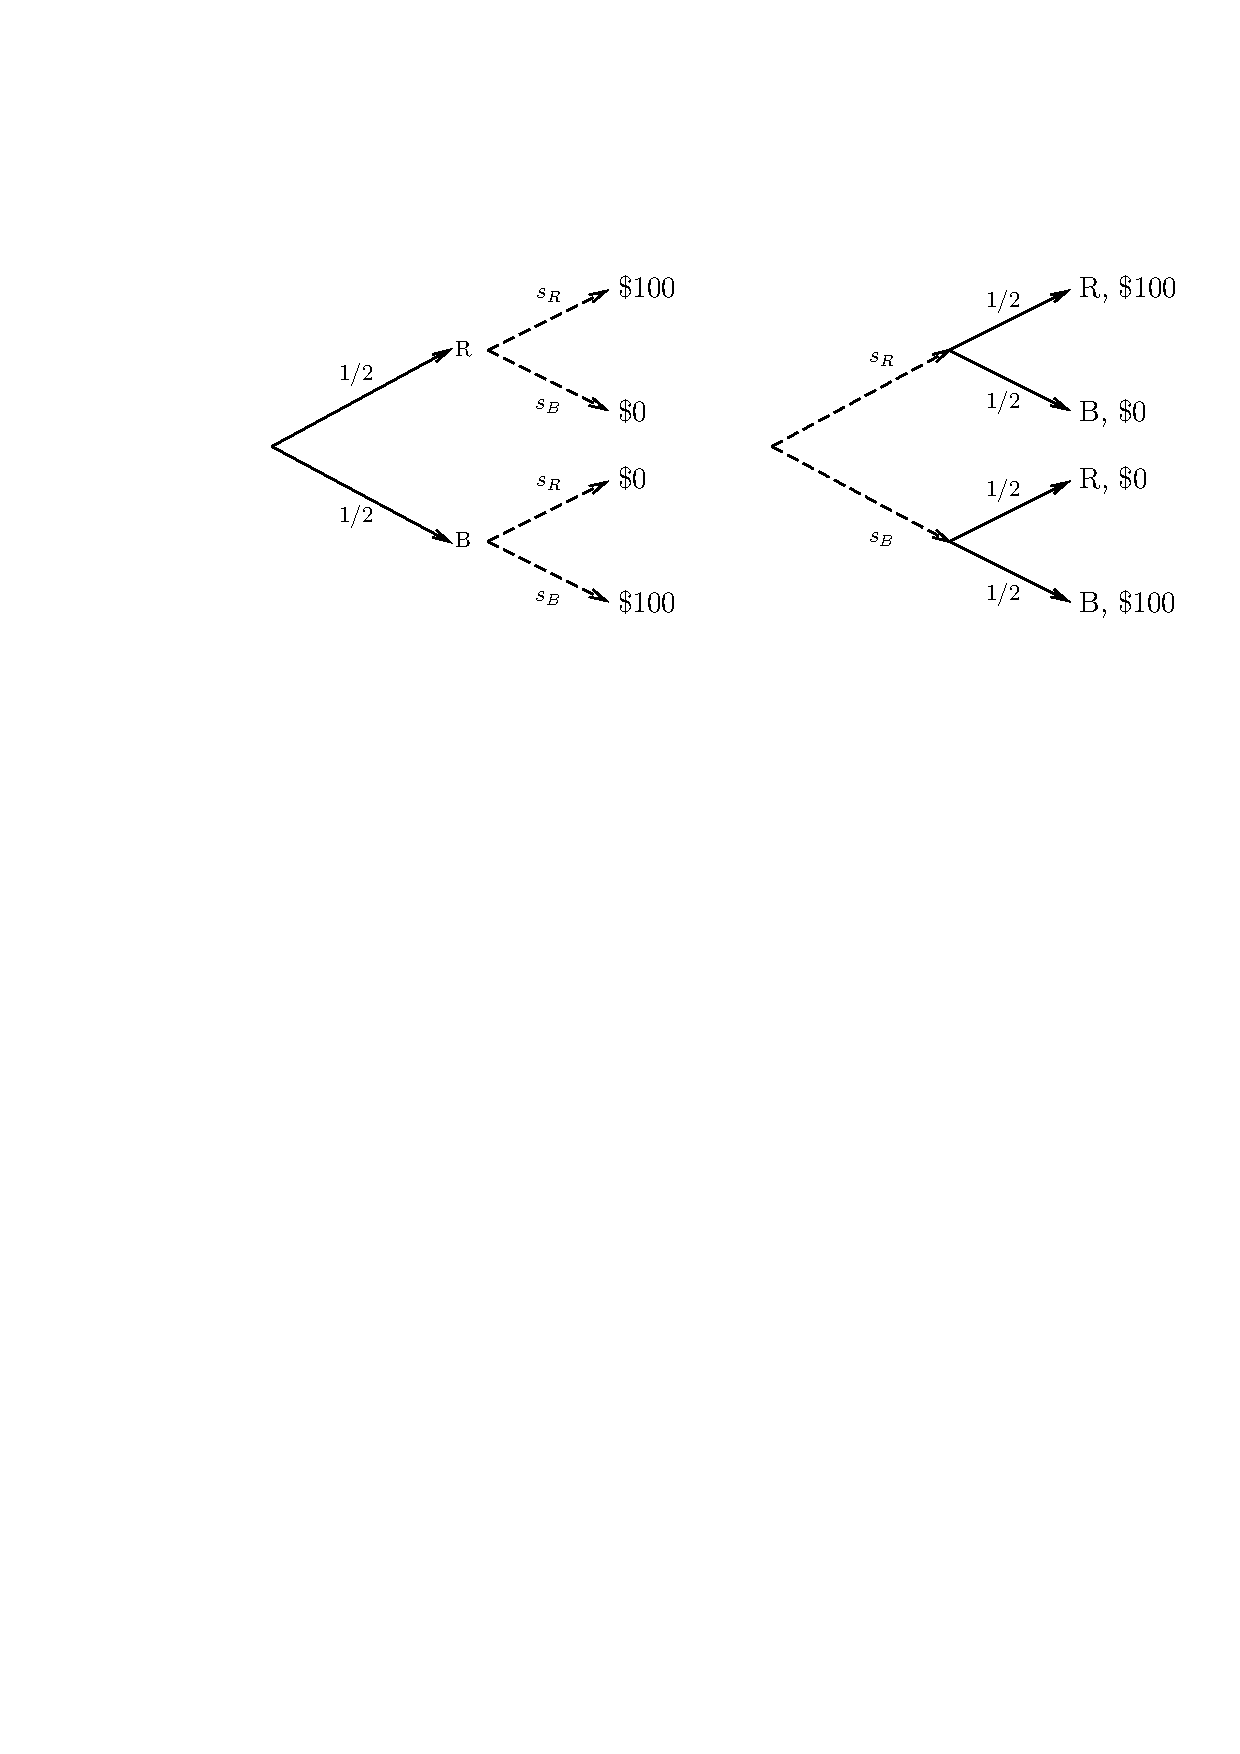
\includegraphics{img/eaep.pdf}
    \caption{There are
two states, in which $s_{R}$ ($s_{B}$) means that red (black) is drawn from
the ambiguous urn. Randomization is represented by solid lines, with
\textquotedblleft R\textquotedblright\ (\textquotedblleft
B\textquotedblright ) representing betting on red (black). The number along
a solid line indicates the objective probability of betting on the
corresponding color.}
\end{figure}


A few papers have noted that the main difference between the two views lies
in \textit{subjective timing}.\footnote{%
Among others, see \cite{EpsteinMarinacciSeo07}; \cite{Bade15}; \cite%
{BaillonHalevyLi15}; \cite{Saito15}; and \cite{OechsslerRauRoomets19}. Note
that subjective timing does not have to be identical to objective timing (if
there is any).} This is easier to explain under the MEU model. Suppose the
individual believes that the number of red balls in the ambiguous urn is
either 30 or 70. Recall that an as-if interpretation of the MEU model is
that the individual believes that nature plays against her. Does she believe
that she randomizes before nature moves or after? If she believes that she
moves first, nature can choose the probability law \textit{based on the
outcome of the coin toss}: If heads (betting on red), the number of red
balls will be 30; otherwise, it is 70. This is consistent with the second
view: Regardless of the outcome of the coin toss, the individual is affected
by ambiguity as in the case without the coin.

This is not true, however, if the individual believes that nature moves
first. If nature moves first, although the number of red balls is unknown,
it \textit{cannot} depend on the outcome of the coin toss. This is therefore
consistent with the first view: Fixing an arbitrary number of red balls, the
coin toss gives the individual a 50-50 lottery between \$100 and \$0. Hence,
the interaction between randomization and ambiguity should depend on the
individual's belief about how the unknown probability law is determined.

Now, return to the service example. In the first situation, before the
individual randomizes, the contracts have pinned down the probability of $%
s_{A}$ and $s_{B}$, although the probability is unknown to the individual.
The view that randomization renders ambiguity irrelevant is more suitable.
In the second situation, it seems more plausible that the effect of
ambiguity is unaffected by randomization: The individual may worry that
after randomization and choosing a service, the details of the service can
still be manipulated.

In the service example, first, there is a natural objective timing of when
the probability law is determined. This is often not the case, and even if
there is a natural objective timing, the individual is free to hold a
different view. Second, the timing is extreme, in the sense that the
probability law is completely pinned down either before randomization or
after. Again, this rarely happens in practice. For example, in the first
situation of the service example, if contracts use words that can be
interpreted in many ways, and \textquotedblleft The service provider
reserves all rights for final explanation\textquotedblright\ is added to
both contracts, how does it change the individual's view of randomization?

Similarly, consider a stylized investment example in which the individual
can either long or short a firm. Suppose she believes that the probability
that the firm succeeds depends on some unknown long-term factor that has
been determined and some unknown short-term factor that will be determined
after she makes a decision. How should randomization interact with ambiguity?

\subsection{Preview of Results}

To study randomization under ambiguity, we adopt the choice domain of \cite%
{AA63} (henceforth AA) and analyze an individual's preference.\footnote{%
We use the original AA choice domain that has two types of mixture
operations. In many papers using the AA choice domain,\ only one mixture
operation, which will be called state-wise randomization in our paper, is
involved, because they assume implicitly that the individual is indifferent
between the two types of mixture operations. See Section \ref{lit} for more
details.} The domain consists of lotteries over acts (\textit{lotteries} for
short henceforth). A lottery is a probability measure (mixed strategy) over
acts. An act assigns to each state of the world a \textit{prize}. A prize is
a probability measure over consequences. Note that this domain does not
require us to describe objectively how the probability law is determined;
this will be subjective and revealed from the individual's preference.

%\FRAME{%
%fhFU}{2.1811in}{2.2883in}{0pt}{\Qcb{A lottery $P$ that yields act $f$ with
%probability $P(f)$ and act $g$ with $P(g)$, in which $f_{i}$ ($g_{i}$) is
%the prize associated with state $s_{i}$ by $f$ ($g$).}}{}{object.bmp}{%
%\special{language "Scientific Word";type "GRAPHIC";maintain-aspect-ratio
%TRUE;display "USEDEF";valid_file "F";width 2.1811in;height 2.2883in;depth
%0pt;original-width 3.2266in;original-height 3.0666in;cropleft "0";croptop
%"1";cropright "1";cropbottom "0";filename 'object.bmp';file-properties
%"XNPEU";}}
\begin{figure}[h!]
  \centering   \label{fig_eaep_intro_to_delete}
    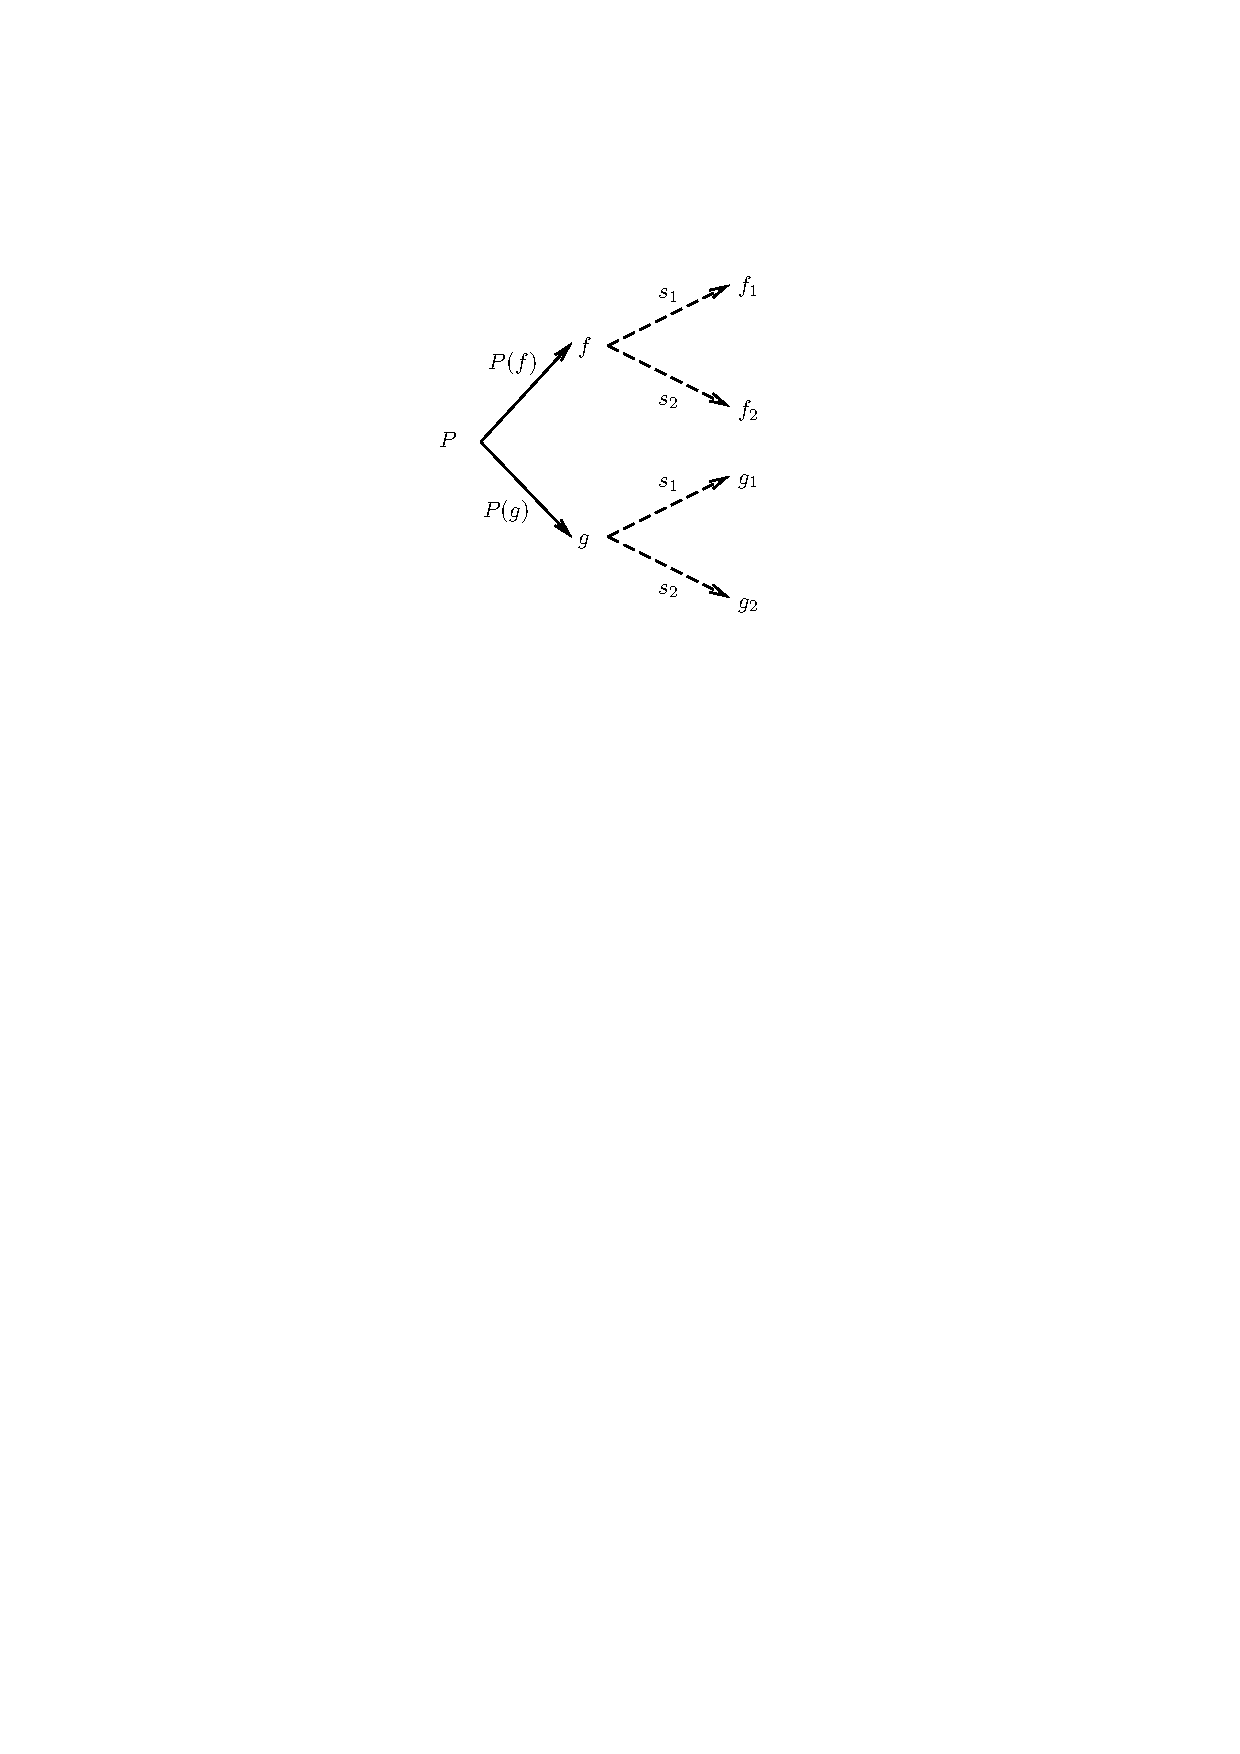
\includegraphics{img/object.pdf}
    \caption{A lottery $P$ that yields act $f$ with
probability $P(f)$ and act $g$ with $P(g)$, in which $f_{i}$ ($g_{i}$) is
the prize associated with state $s_{i}$ by $f$ ($g$).}
\end{figure}



We incorporate ideas from \cite{GilboaSchmeidler89} and first- and
second-order stochastic dominance to relax AA's axioms. Our main theorem
characterizes the following representation of the individual's preference
over lotteries, the \textit{double maxmin expected utility} (DMEU)
representation: For each lottery $P$,%
\begin{equation*}
W(P)=\min_{M\in \mathcal{M}}~\int_{\mathcal{F}}\left( \underset{\mu \in M}{%
\min }~\int_{\mathcal{S}}u(f)~d\mu \right) ~dP,
\end{equation*}%
in which each $M\in \mathcal{M}$ is a set of priors, and $u(f(s))$ is the
utility of the prize that an act $f$ assigns to state $s$. Each $M\in 
\mathcal{M}$ is called a \textit{scenario}. The individual believes that
before she randomizes, nature, which plays against her, has chosen a
scenario (although unknown to her) from $\mathcal{M}$. After she randomizes,
nature will choose a prior $\mu $ from that scenario.

%\FRAME{fhFU}{4.5999in}{4.8438in}{0pt}{\Qcb{\label{fig_intro_eg1}There are
%two scenarios. For example, $(0.3,0.7)$ is the scenario with 30 red balls
%and 70 black balls in the ambiguous urn. There is only one prior in each
%scenario. In state $s_{R}$ ($s_{B}$), the ball drawn is red (black). In each
%scenario, randomization and state revelation constitute a compound lottery
%that yields \$100 and \$0 with equal probability.}}{}{intro_eg1.bmp}{\special%
%{language "Scientific Word";type "GRAPHIC";maintain-aspect-ratio
%TRUE;display "USEDEF";valid_file "F";width 4.5999in;height 4.8438in;depth
%0pt;original-width 3.1401in;original-height 3.467in;cropleft "0";croptop
%"1";cropright "1";cropbottom "0";filename 'intro_eg1.bmp';file-properties
%"XNPEU";}}

\begin{figure}[h!]
  \centering   \label{fig_intro_eg1}
    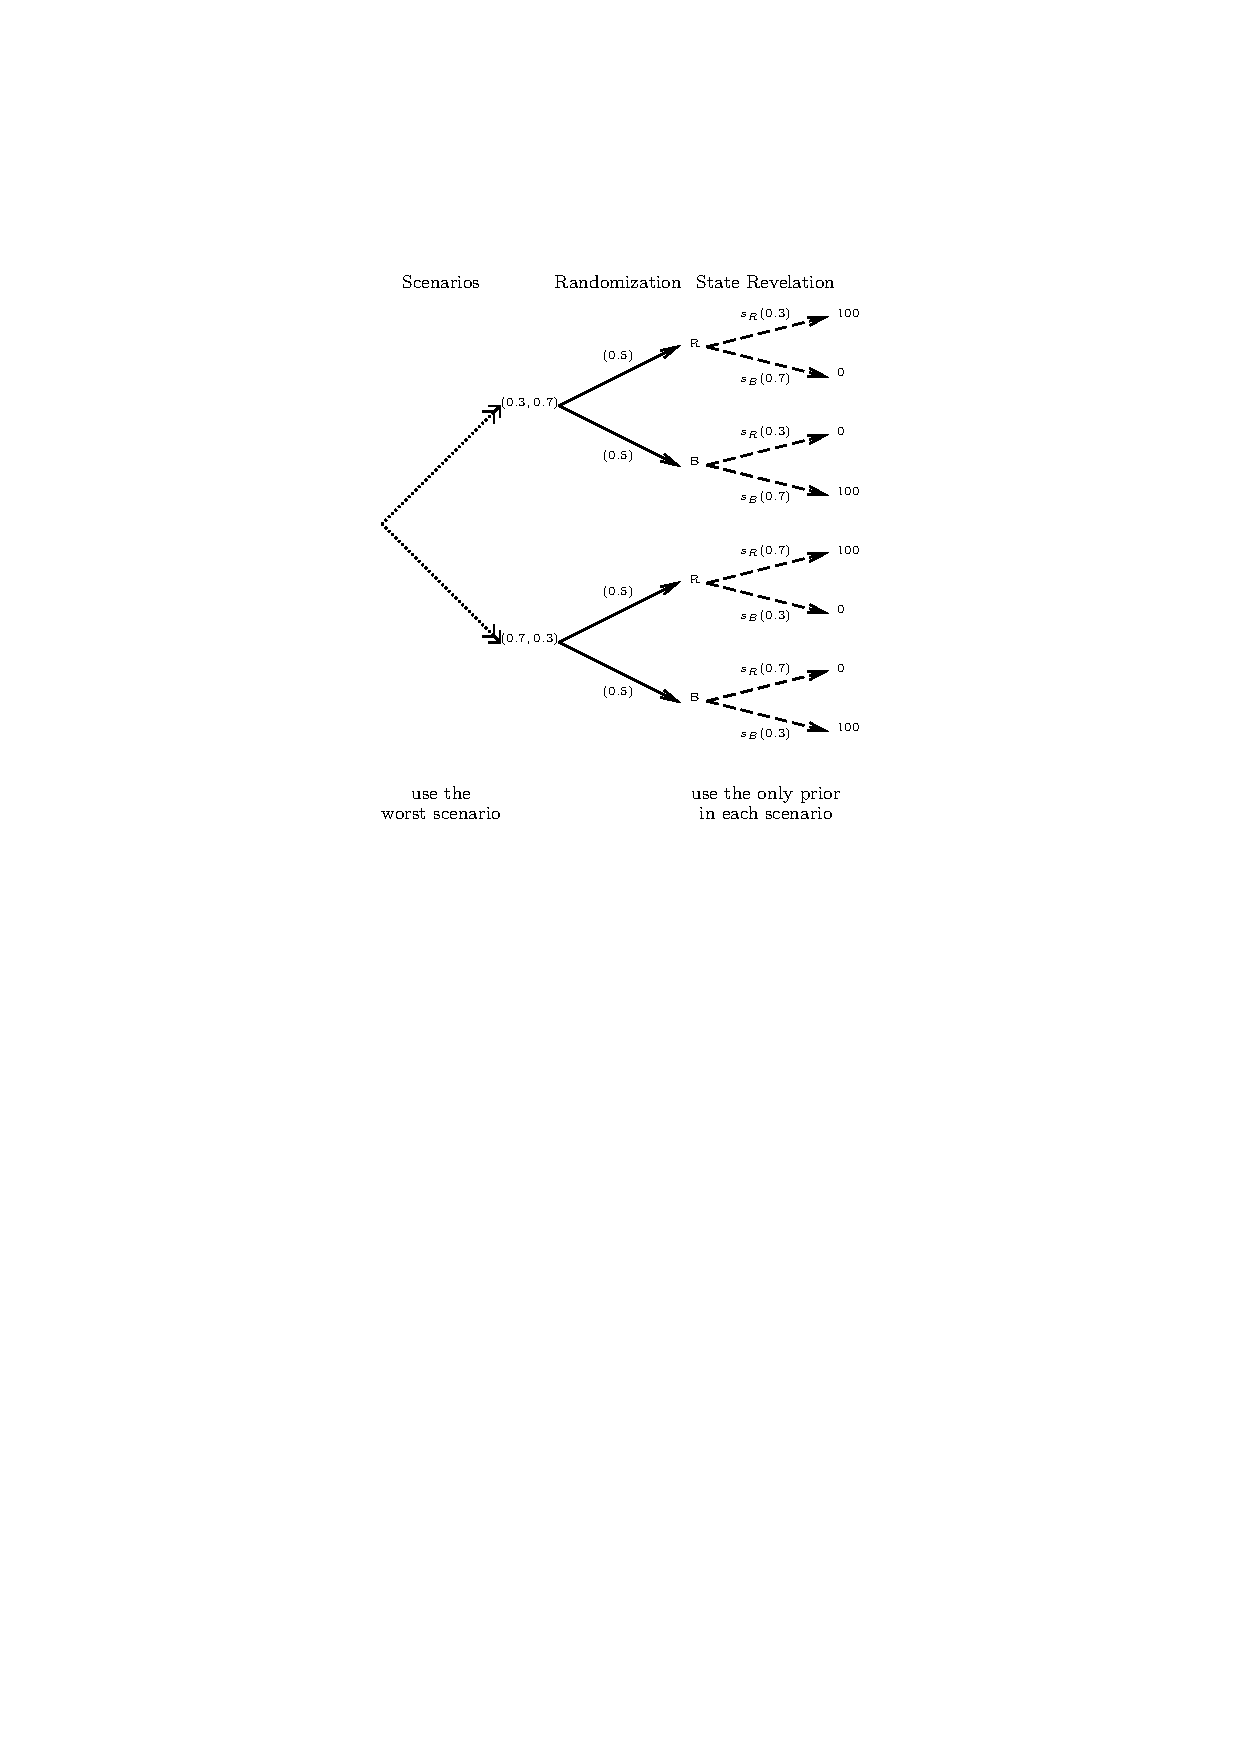
\includegraphics{img/intro_eg1.pdf}
    \caption{There are
two scenarios. For example, $(0.3,0.7)$ is the scenario with 30 red balls
and 70 black balls in the ambiguous urn. There is only one prior in each
scenario. In state $s_{R}$ ($s_{B}$), the ball drawn is red (black). In each
scenario, randomization and state revelation constitute a compound lottery
that yields \$100 and \$0 with equal probability.}
\end{figure}


Figures \ref{fig_intro_eg1}--\ref{fig_intro_eg3} illustrate how the DMEU
representation reveals the individual's belief about the determination of
the unknown probability law and about the interaction between randomization
and ambiguity. Figure \ref{fig_intro_eg1} depicts the urn example assuming
that the individual believes that randomization eliminates the effect of\
ambiguity, in which every scenario $M\in \mathcal{M}$ is a singleton. Figure %
\ref{fig_intro_eg2} depicts the urn example assuming that the individual
believes that the effect of ambiguity is unaffected by randomization, in
which case $\mathcal{M}$ is a singleton and $M\in \mathcal{M}$ is not.

%\FRAME{fhFU}{4.3491in}{2.8651in}{0pt}{\Qcb{\label{fig_intro_eg2}The only
%scenario contains two priors (either 30 or 70 red balls in the ambiguous
%urn). The worst prior within the scenario depends on the realization of
%randomization.}}{}{intro_eg2.bmp}{\special{language "Scientific Word";type
%"GRAPHIC";maintain-aspect-ratio TRUE;display "USEDEF";valid_file "F";width
%4.3491in;height 2.8651in;depth 0pt;original-width 3.0865in;original-height
%2.0271in;cropleft "0";croptop "1";cropright "1";cropbottom "0";filename
%'intro_eg2.bmp';file-properties "XNPEU";}}

\begin{figure}[h!]
  \centering   \label{fig_intro_eg2}
    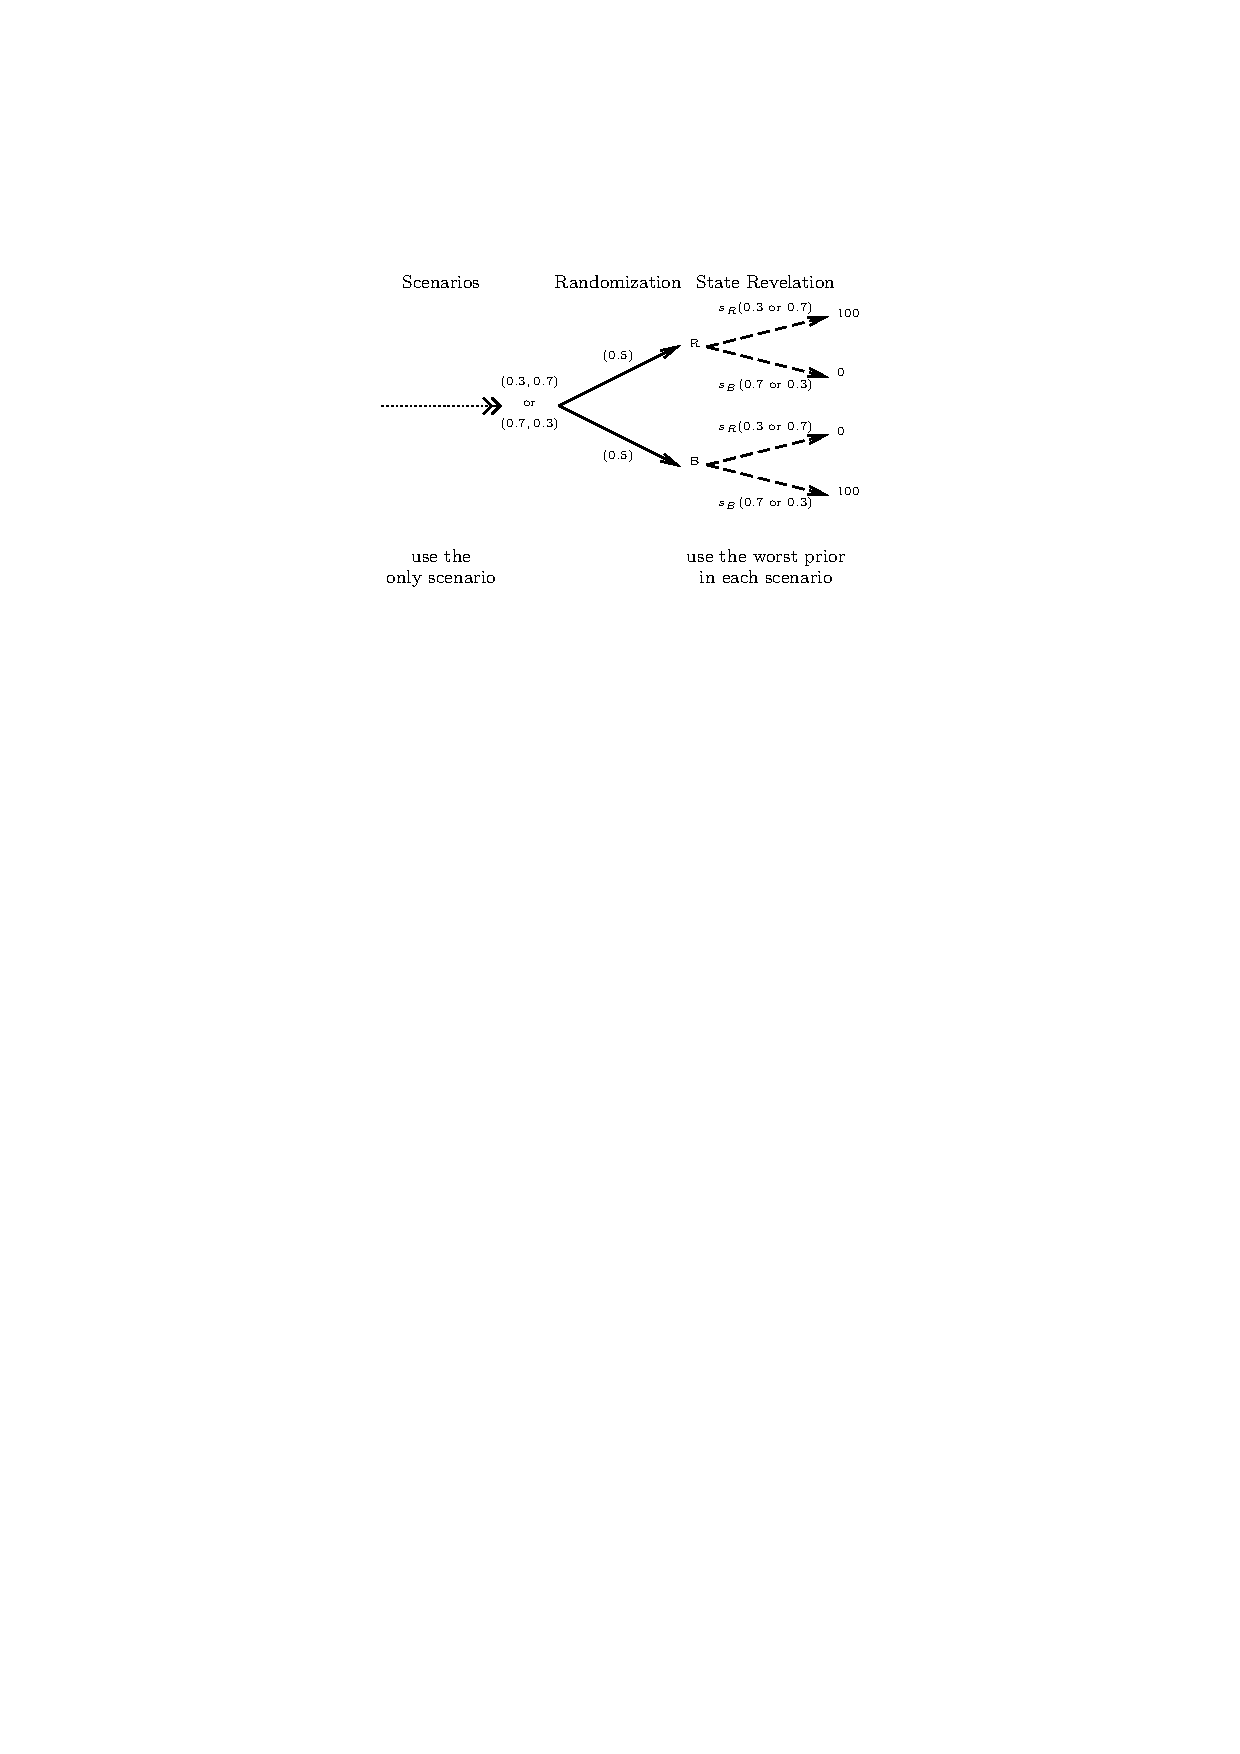
\includegraphics{img/intro_eg2.pdf}
    \caption{The only
scenario contains two priors (either 30 or 70 red balls in the ambiguous
urn). The worst prior within the scenario depends on the realization of
randomization.}
\end{figure}

Figure \ref{fig_intro_eg3} is the investment example, in which the
probability that the firm succeeds depends on some unknown long-term and
short-term factors. This example shows that randomization may partially
eliminate the effect of\ ambiguity---it helps eliminate the effect of\
ambiguity across scenarios, but not across probability laws within a
scenario. The individual believes that one unknown scenario in $\mathcal{M}%
=\{M_{G},M_{N},M_{B}\}$ has occured before she chooses. Both scenarios $%
M_{G} $ (good long-term factor) and $M_{B}$ (bad long-term factor) are
singletons---the long-term factor alone determines the probability law. In
scenario $M_{N}$, how likely the firm is to succeed also depends on the
short-term factor, which is not yet determined. In this case, randomization
eliminates the effect of ambiguity across scenarios $M_{G}$ and $M_{B}$, but
not within $M_{N}$.\footnote{%
A more detailed discussion follows Theorem \ref{special}.}

%\FRAME{fhFU}{4.1632in}{5.2598in}{0pt}{\Qcb{\label{fig_intro_eg3}In the good
%scenario $M_{G}$, the firm will profit (state $s_{p}$) with probability $1$.
%In the bad scenario $M_{B}$, the firm will profit with probability $0$. In
%the neutral scenario $M_{N}$, the probability that the firm profits is
%either $0.3$ or $0.7$, which will be determined after randomization.}}{}{%
%intro_eg3.bmp}{\special{language "Scientific Word";type
%"GRAPHIC";maintain-aspect-ratio TRUE;display "USEDEF";valid_file "F";width
%4.1632in;height 5.2598in;depth 0pt;original-width 3.6997in;original-height
%3.4731in;cropleft "0";croptop "1";cropright "1";cropbottom "0";filename
%'intro_eg3.bmp';file-properties "XNPEU";}}

\begin{figure}[h!]
  \centering   \label{fig_intro_eg3}
    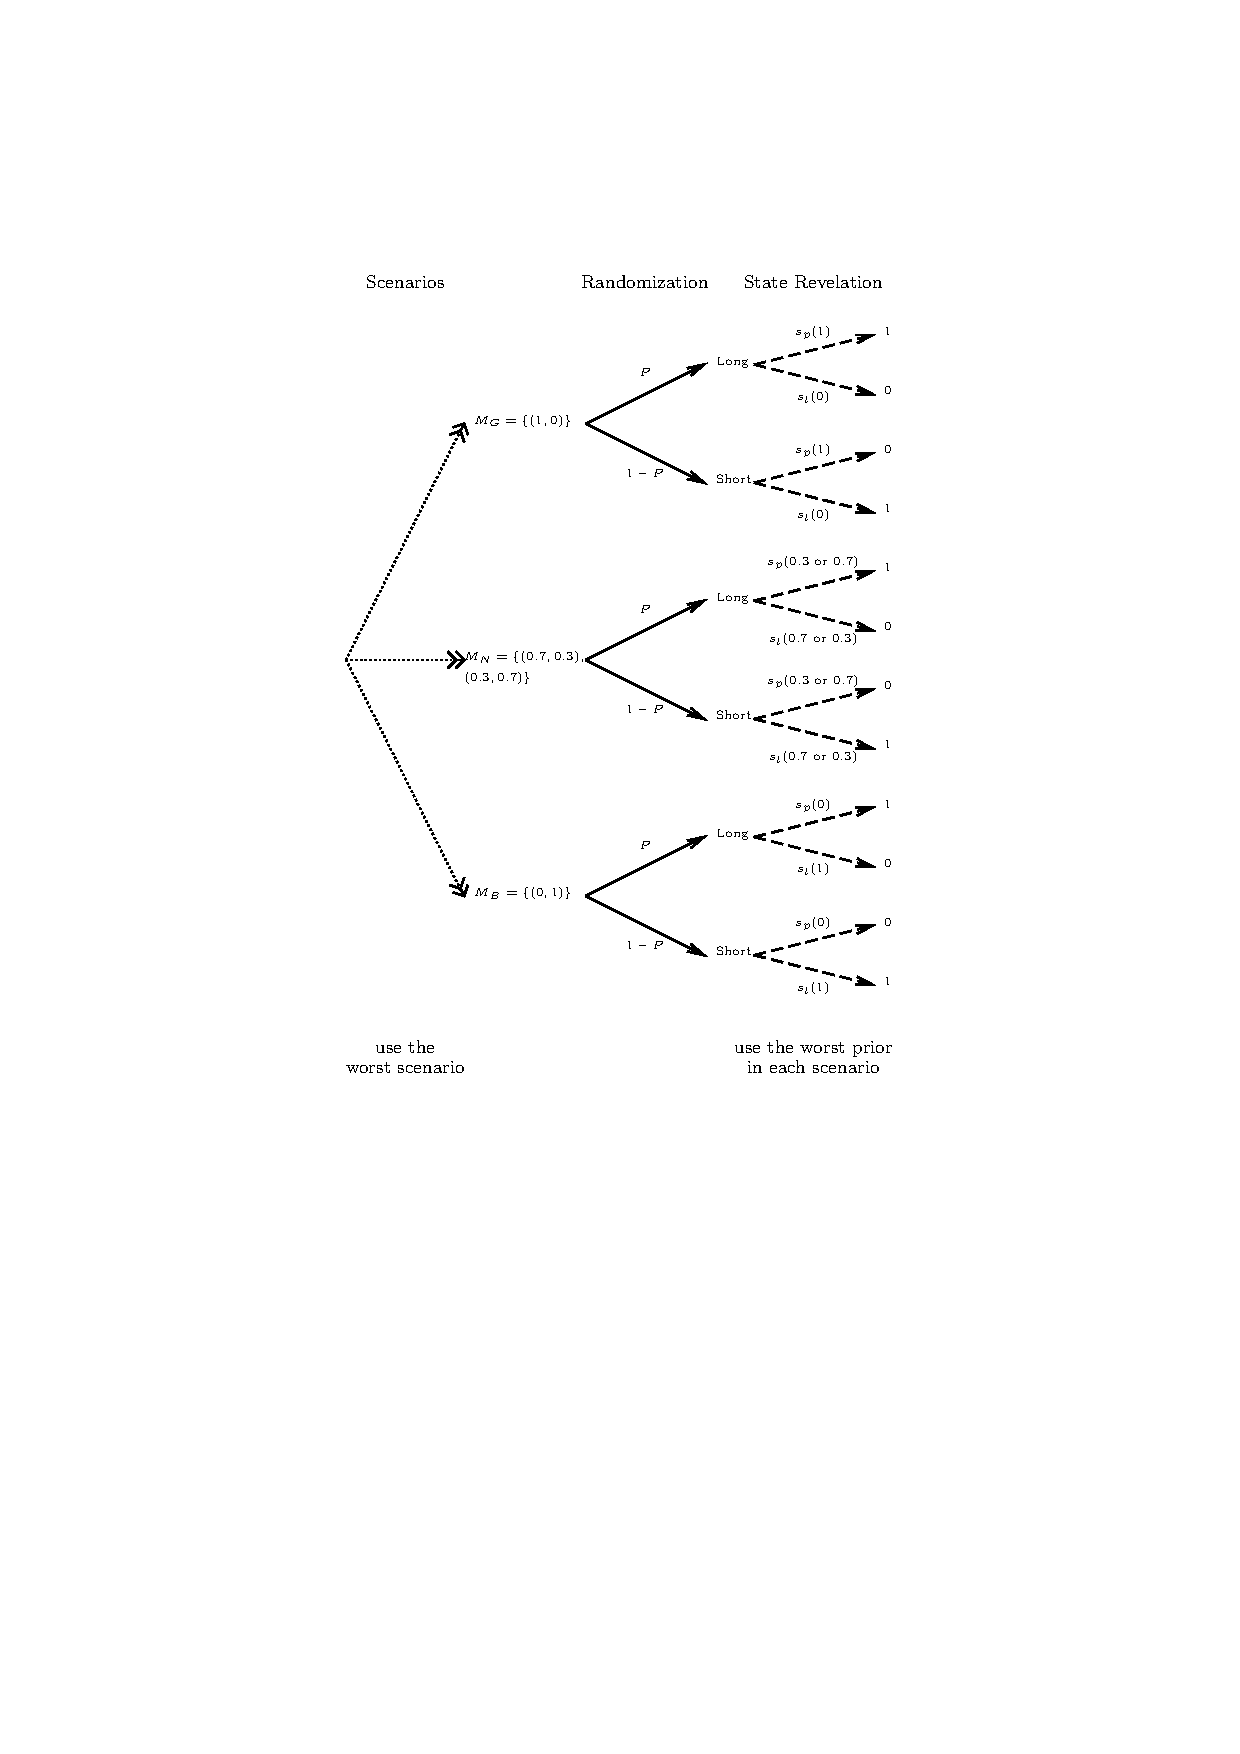
\includegraphics{img/intro_eg3.pdf}
    \caption{In the good
scenario $M_{G}$, the firm will profit (state $s_{p}$) with probability $1$.
In the bad scenario $M_{B}$, the firm will profit with probability $0$. In
the neutral scenario $M_{N}$, the probability that the firm profits is
either $0.3$ or $0.7$, which will be determined after randomization.}
\end{figure}


We discuss the related literature below, and more discussion can be found in
Section \ref{lit}. The closest paper to ours is \cite{Saito15}. Saito also
studies an axiomatic model in which the ambiguity-averse individual may have
a preference for randomization. His model uses a convex combination to
combine the two extreme timing beliefs. We will show that his model is a
special case of ours. In addition to models of ambiguity aversion, there are
other models of preference for randomization under different choice domains
with different motivations, such as \cite{Machina85}; \cite%
{Cerreia-VioglioDillenbergerOrtoleva15}; \cite{FudenbergIijimaStrzalecki15};
and \cite{Cerreia-VioglioDillenbergerOrtolevaEtAl19},\ among others.

Several papers have also examined representations of preferences that
involve collections of sets of priors. \cite{LehrerTeper11} study a
representation called the multiple multiple-priors representation, which
allows for violations of completeness and transitivity. \cite%
{FrickIijimaLeYaouanq19} propose the Boolean expected utility
representation, in which the belief the individual uses to evaluate an act
is the most pessimistic prior from the most optimistic set of priors.

Empirical studies have examined whether individuals strictly prefer to
randomize. For example, \cite{DominiakSchnedler11}; \cite{AgranovOrtoleva17}%
; \cite{DwengerKublerWeizsacker16}; \cite{OechsslerRauRoomets19}; \cite%
{ChewMiaoShenEtAl19}; and \cite{ZhangZhong19}. Many of them find a
nonnegligible number of subjects who strictly prefer to randomize, but some
do not. This is consistent with our theory: The individual may strictly
prefer to randomize in some choice problems but not in others, and how
desirable randomization appears to her depends on her timing beliefs.

Preference for randomization is also an important topic in preference
elicitation. For example, our main idea that the individual's evaluation of
a lottery depends on her belief about how the unknown probability law is
determined has also appeared in the research on random incentive mechanisms. 
\cite{Bade15}\ and \cite{BaillonHalevyLi15} argue that ambiguity-averse
participants may use the randomization device to hedge, and thus the
incentive compatibility of the random incentive mechanism may be affected. 
\cite{Kuzmics17} also points out the difficulty of preference elicitation
when individuals face ambiguity: Individuals with non-SEU preferences may
end up behaving as if they are SEU maximizers in preference elicitation
choice problems.

Finally, many papers have studied ambiguity and robustness in different
areas of economics. As mentioned earlier, how mixed strategies should be
introduced and evaluated has been an issue. Our results offer some new
insights to this issue. We leave the detailed discussion to the end of the
paper.

The paper proceeds as follows. Section \ref{mainsection} introduces the
choice domain, mixture operations, and a variant of AA's characterization of
the subjective expected utility representation. Section \ref{compare}
presents the main axioms, the DMEU representation, and the main results.
Section \ref{threeaxioms} examines three special cases of the DMEU. Section %
\ref{lit} discusses the related literature.

\section{Preliminaries}

\label{mainsection}The set of consequences is a compact Polish space $%
\mathcal{X}$.\footnote{%
A Polish space is a complete separable metric space.} Let $\Delta (\mathcal{X%
})$ be the set of Borel probability measures on $\mathcal{X}$, endowed with
the topology of weak convergence. Elements of $\Delta (\mathcal{X})$ are
called \textit{prizes}. Let $\mathcal{S}=\{s_{1},\dots ,s_{n}\}$ be a finite
set of states. An \textit{act} $f:\mathcal{S}\rightarrow \Delta (\mathcal{X}%
) $ is a function that assigns a prize to each state. For each state $s_{i}$%
, we write $f_{i}$ instead of $f(s_{i})$ for simplicity. Let $\mathcal{F}$
denote the set of all acts, endowed with the product topology. Let $\Delta (%
\mathcal{F})$, the set of Borel probability measures on $\mathcal{F}$,
denote the set of all \textit{lotteries}, endowed with the topology of weak
convergence. Henceforth, when we say a set of acts, we mean a Borel
measurable subset of $\mathcal{F}$. The support of a lottery $P\in \Delta (%
\mathcal{F})$, denoted by supp$(P)$, is the smallest closed set of acts $%
F\subset \mathcal{F}$ such that $P(F)=1$. The individual has a binary
relation/preference $\succsim $ on $\Delta (\mathcal{F})$. We denote the
asymmetric part of $\succsim $ by $\succ $ and the symmetric part by $\sim $.

A lottery represents randomization over acts. Following randomization, the
individual receives an act. Next, a state is \textit{revealed to the
individual}, after which the act assigns the prize associated with the
realized state to the individual. Finally, as the prize's risk resolves, the
individual receives a consequence (see Figure \ref{object}).

%\FRAME{fhFU}{2.1811in}{2.2883in}{0pt}{\Qcb{\label{object}An example of a
%lottery $P$, in which $f$ and $g$ are two acts, $\{s_{1},s_{2}\}$ is the
%state space, and $f_{i}$ ($g_{i}$) is the prize associated with state $s_{i}$
%by $f$ ($g$).}}{}{object.bmp}{\special{language "Scientific Word";type
%"GRAPHIC";maintain-aspect-ratio TRUE;display "USEDEF";valid_file "F";width
%2.1811in;height 2.2883in;depth 0pt;original-width 3.2266in;original-height
%3.0666in;cropleft "0";croptop "1";cropright "1";cropbottom "0";filename
%'object.bmp';file-properties "XNPEU";}}

\begin{figure}[h!]
  \centering   \label{object}
    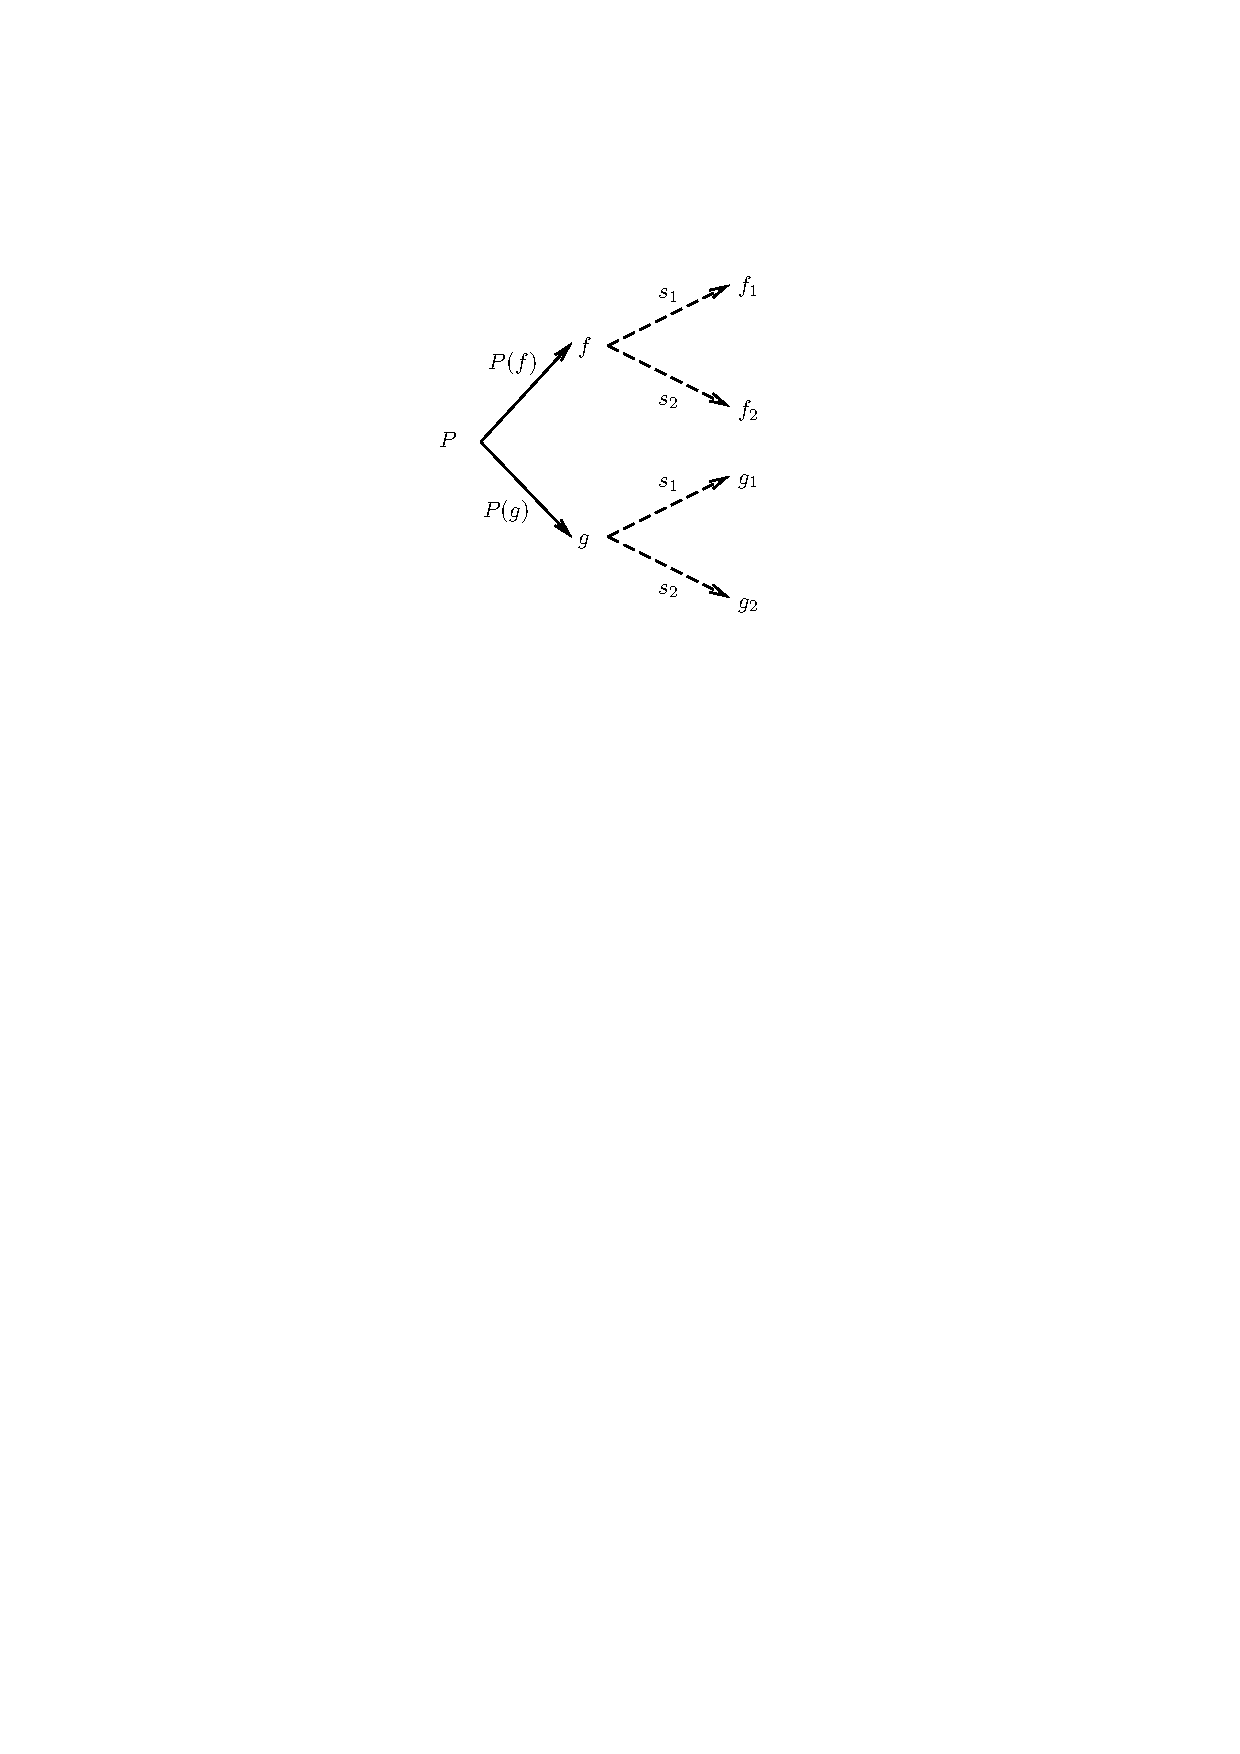
\includegraphics{img/object.pdf}
    \caption{An example of a
lottery $P$, in which $f$ and $g$ are two acts, $\{s_{1},s_{2}\}$ is the
state space, and $f_{i}$ ($g_{i}$) is the prize associated with state $s_{i}$
by $f$ ($g$).}
\end{figure}



Lotteries are denoted by $P,Q,R$, acts are denoted by $f,g,h$, and prizes
are denoted by $p,q,r$. A degenerate lottery that assigns probability $1$ to
an act $f$ is identified with $f$. If an act yields the same prize $p$ in
all states, the act is called a \textit{constant act}, and is identified
with $p$. If a prize assigns probability $1$ to a consequence $x$, we denote
the prize by $\delta _{x}$.

We assume throughout the paper that $\succsim $ is nontrivial: There exist
some lotteries $P$ and $Q$ such that $P\succ Q$.

\subsection{Randomization and State-wise Randomization}

\label{rswr}We distinguish between two kinds of mixture operations. First,
the \textit{randomization} between lotteries $P$ and $Q$ with probability $%
\alpha \in \lbrack 0,1]$, denoted by $\alpha P+(1-\alpha )Q$, is a lottery
that assigns probability $\alpha P(F)+(1-\alpha )Q(F)$ to each set of acts $%
F\subset \mathcal{F}$. The second kind of mixture operation is state by
state and for acts. The \textit{state-wise randomization} between acts $f$
and $g$ with probability $\alpha \in \lbrack 0,1]$, denoted by $\alpha
f+_{sw}(1-\alpha )g$, is an act that assigns the prize $\alpha
f_{i}+(1-\alpha )g_{i}$ to each state $s_{i}$ (see Figure \ref{fig_rswr}).%
\footnote{%
Here, $\alpha f_{i}+(1-\alpha )g_{i}$ is the standard mixture between prizes
(probability measures over consequences) used in expected utility theory.
With an abuse of notation, this mixture is also denoted by \textquotedblleft 
$+$.\textquotedblright\ In most other places of the paper, however,
\textquotedblleft $+$\textquotedblright\ represents randomization between
lotteries.}

%\FRAME{fhFU}{4.868in}{2.4751in}{0pt}{\Qcb{\label{fig_rswr}Suppose there are
%two states: $s_{1}$ and $s_{2}$. The left-hand lottery is the randomization
%with probability $\protect\alpha $ between acts (degenerate lotteries) $f$
%and $g$. The right-hand act is the state-wise randomization with probability 
%$\protect\alpha $ between acts $f$ and $g$.}}{}{eaep_main.bmp}{\special%
%{language "Scientific Word";type "GRAPHIC";maintain-aspect-ratio
%TRUE;display "USEDEF";valid_file "F";width 4.868in;height 2.4751in;depth
%0pt;original-width 5.4059in;original-height 2.6939in;cropleft "0";croptop
%"1";cropright "1";cropbottom "0";filename 'eaep_main.bmp';file-properties
%"XNPEU";}}

\begin{figure}[h!]
  \centering   \label{fig_rswr}
    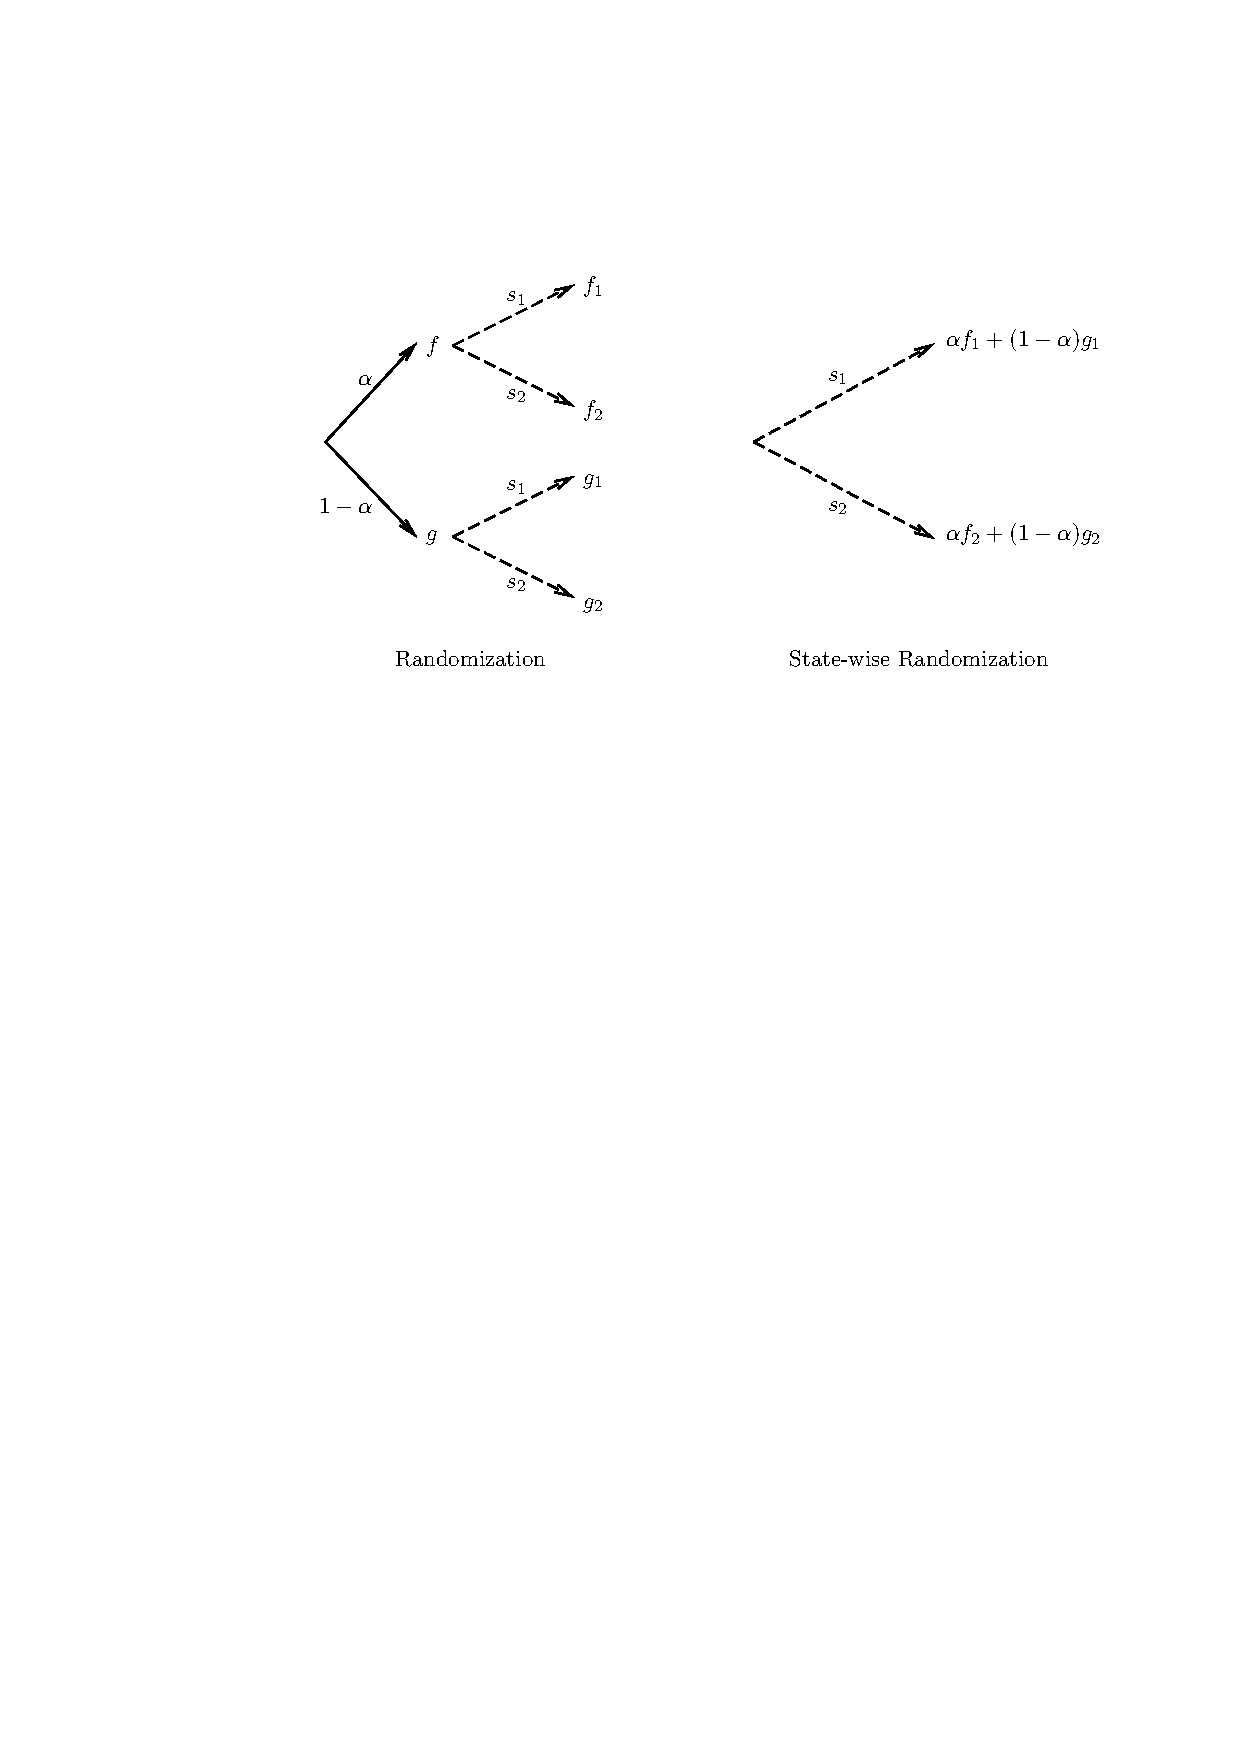
\includegraphics{img/eaep_main.pdf}
    \caption{Suppose there are
two states: $s_{1}$ and $s_{2}$. The left-hand lottery is the randomization
with probability $\protect\alpha $ between acts (degenerate lotteries) $f$
and $g$. The right-hand act is the state-wise randomization with probability 
$\protect\alpha $ between acts $f$ and $g$.}
\end{figure}


The difference between the two mixture operations is obvious, but one useful
way to understand it is to consider randomization as a mixture performed 
\textit{before} the state is revealed to the individual, and state-wise
randomization a mixture performed \textit{after} the state is revealed. In
the urn experiment, before a ball is drawn, the individual tosses a fair
coin and bets on red being drawn from the ambiguous urn if heads and black
if tails. This is randomization and is done before the color of the drawn
ball is revealed to the individual. As discussed in Section \ref{intro},
whether such randomization eliminates the effect of\ ambiguity depends on
the individual's subjective timing belief.

In contrast, suppose the individual first observes the color of the ball
drawn, and then tosses the coin and bets accordingly. This will generate an
act that yields a 50-50 lottery between \$100 and \$0 in all states, $s_{R}$
(red is drawn) and $s_{B}$ (black is drawn), which is exactly the 50-50
state-wise randomization between betting on red and black (see also the
right-hand side of Figures \ref{fig_eaep_intro} and \ref{fig_rswr}). Since
the prize is identical in all states, this 50-50 state-wise randomization
eliminates the effect of\ ambiguity, \textit{regardless of the individual's
belief about how the unknown probability law is determined}. Intuitively, if
the mixture happens after the state is revealed, nature must have determined
the probability law. Hence, the individual's belief about how the
probability law is determined no longer matters; more importantly, under the
same mixture probability, state-wise randomization should be (weakly) more
effective in eliminating the effect of ambiguity than randomization.

\subsection{Subjective Expected Utility}

AA provide a characterization of the subjective expected utility
representation. We introduce a variant of it that will be useful in
motivating our axioms in Section \ref{compare}. The first four axioms are
restatements of AA's axioms and assumptions using our terminology and
notation.

\begin{axiom}
(Weak Order) The preference $\succsim $ is complete and transitive.
\end{axiom}

\begin{axiom}
(Continuity) For any $P\in \Delta (\mathcal{F})$, $\{Q\in \Delta (\mathcal{F}%
):Q\succsim P\}$ and $\{Q\in \Delta (\mathcal{F}):P\succsim Q\}$ are closed.
\end{axiom}

The first two axioms are basic. The next three axioms are the ones we want
to relax later.

\begin{axiom}
(Independence) For any $P,Q,R\in \Delta (\mathcal{F})$ and $\alpha \in (0,1)$%
, $P\succsim Q$ if and only if $\alpha P+(1-\alpha )R\succsim \alpha
Q+(1-\alpha )R$.
\end{axiom}

\begin{axiom}
(State-wise Independence) For any $f,g,h\in \mathcal{F}$ and $\alpha \in
(0,1)$, $f\succsim g$ if and only if $\alpha f+_{sw}(1-\alpha )h\succsim
\alpha g+_{sw}(1-\alpha )h$.
\end{axiom}

To state the last axiom, we need the following notation. For each lottery $P$%
, let $f^{P}$ denote the act such that%
\begin{equation}
f_{i}^{P}(X)=\int_{\mathcal{F}}f_{i}(X)~dP,  \label{projection}
\end{equation}%
for any $i\in \{1,\dots ,n\}$ and measurable set of consequences $X\subset 
\mathcal{X}$. By construction, the lottery $P$ is converted into an act $%
f^{P}$ state by state via reduction of compound lotteries. For example,
suppose the support of $P$ is finite. Fixing any state $s_{i}$, $f_{i}^{P}$
is the mixture of prizes weighted by $P$, $\sum_{f\in \text{supp}%
(P)}P(f)\cdot f_{i}$, which is a standard compound lottery in expected
utility theory. To put it differently, if we convert all randomization in $P$
into state-wise randomization, we obtain $f^{P}$.

\begin{axiom}
(Strong Dominance) For any $P,Q\in \Delta (\mathcal{F})$, if $%
f_{i}^{P}\succsim f_{i}^{Q}$ for any $i$, $P\succsim Q$.
\end{axiom}

This axiom combines AA's two axioms, \textit{Monotonicity in Prizes} and 
\textit{Reversal of Order in Compound Lotteries}. \textit{Monotonicity in
Prizes} requires that for any two acts $f$ and $g$, if $f_{i}\succsim g_{i}$
for every $i$, $f\succsim g$. \textit{Reversal of Order in Compound Lotteries%
} requires that $f^{P}\sim P$. Therefore, \textit{Strong Dominance} requires
that the individual be indifferent between randomization and state-wise
randomization. The lemma below emphasizes this, and illustrates some basic
relation between \textit{Independence}, \textit{State-wise Independence},
and \textit{Strong Dominance}. All omitted proofs can be found in the
Appendix.

\begin{lemma}
\label{triangle}Suppose $\succsim $ satisfies Weak Order. The following
statements are true:

\begin{enumerate}
\item For any lotteries $P,Q$ and $\alpha \in \lbrack 0,1]$, Strong
Dominance implies that $\alpha P+(1-\alpha )Q\sim f^{\alpha P+(1-\alpha
)Q}\sim \alpha f^{P}+(1-\alpha )f^{Q}\sim \alpha f^{P}+_{sw}(1-\alpha )f^{Q}$%
;

\item Under Strong Dominance, Independence is equivalent to State-wise
Independence.
\end{enumerate}
\end{lemma}

The axioms above characterize the subjective expected utility
representation. A function $u:\Delta (\mathcal{X})\rightarrow \mathbb{R}$ is
an \textit{expected utility function} if for any prize $p$,%
\begin{equation*}
u(p)=\int_{\mathcal{X}}u(\delta _{x})~dp.
\end{equation*}%
Let $\Delta (\mathcal{S})$ denote the set of probability measures on $%
\mathcal{S}$.

\begin{definition}
The individual's preference $\succsim $ has a \textit{subjective expected
utility} (SEU) representation if there exists a continuous expected utility
function $u:\Delta (\mathcal{X})\rightarrow \mathbb{R}$ and $\mu \in \Delta (%
\mathcal{S})$ such that the following function $W$ represents $\succsim $:%
\begin{equation}
W(P)=\int_{\mathcal{F}}\left( \int_{\mathcal{S}}u(f)~d\mu \right) ~dP.
\label{seu}
\end{equation}
\end{definition}

Since we assume that $\succsim $ is nontrivial, implicitly in the definition
above, $u$ is not constant. We will not mention this again for our other
representations, but similar implicit assumptions apply to them as well.

When $\succsim $ has an SEU representation, the individual is indifferent
between randomization and state-wise randomization, which is reflected in
the following equations:%
\begin{equation*}
W(P)=\int_{\mathcal{F}}\left( \int_{\mathcal{S}}u(f)~d\mu \right) ~dP=\int_{%
\mathcal{S}}\left( \int_{\mathcal{F}}u(f)~dP\right) ~d\mu =\int_{\mathcal{S}%
}u(f^{P})~d\mu =W(f^{P}).
\end{equation*}%
We say that an SEU representation is unique if in (\ref{seu}), $u$ is unique
up to a positive affine transformation and $\mu $ is unique. The theorem
below restates AA's main representation result.

\begin{theorem}
\label{aa}(\cite{AA63}) The individual's preference $\succsim $ has an SEU
representation if and only if it satisfies Weak Order, Continuity,
Independence, State-wise Independence, and Strong Dominance. Furthermore,
the SEU representation is unique.
\end{theorem}

Because \textit{Strong Dominance} holds, Lemma \ref{triangle} implies that
one of the two axioms,\textit{\ Independence} or \textit{State-wise
Independence}, is redundant. Stating the theorem in this way, however, helps
us motivate the relaxations we introduce below.

\section{Axioms and the Representation}

\label{compare}Three axioms will be relaxed. Observing that state-wise
randomization may render ambiguity irrelevant because of hedging (as
discussed in Section \ref{rswr}), \cite{GilboaSchmeidler89} propose a
relaxation of their independence assumption, which is \textit{State-wise
Independence} in our setting, to capture this. They allow the individual's
preference to be convex so that she may strictly prefer state-wise
randomization; meanwhile, constant acts should continue to satisfy the
independence assumption, because constant acts do not provide hedging
opportunities. We relax \textit{State-wise Independence} in the same way.

We also want to relax \textit{Independence} so that the individual may
strictly prefer randomization. In the urn experiment, if the individual
agrees with Raiffa's (1961) argument, or in the service example, if the
details of the services are precisely stated in contracts beforehand,
randomization can render ambiguity irrelevant. In the investment example in
Figure \ref{fig_intro_eg3}, randomization partially eliminates\ the effect
of\ ambiguity, which also violates \textit{Independence}. We relax \textit{%
Independence} following the way \cite{GilboaSchmeidler89} relax \textit{%
State-wise Independence}.

We say that a lottery $P$ preserves\textit{\ Independence} if for any
lotteries $Q,R$ and $\alpha \in (0,1)$, $Q\succsim R$ if and only if $\alpha
Q+(1-\alpha )P\succsim \alpha R+(1-\alpha )P$. We say that an act $f$
preserves \textit{State-wise Independence} if for any acts $g,h$ and $\alpha
\in (0,1)$, $g\succsim h$ if and only if $\alpha g+_{sw}(1-\alpha )f\succsim
\alpha h+_{sw}(1-\alpha )f$.

\begin{axiom}
(Preference for Randomization)

\begin{enumerate}
\item[(i)] For any $P,Q\in \Delta (\mathcal{F})$ and $\alpha \in \lbrack
0,1] $, $P\succsim Q$ implies $\alpha P+(1-\alpha )Q\succsim Q$;

\item[(ii)] Every constant act preserves Independence.
\end{enumerate}
\end{axiom}

\begin{axiom}
(Preference for State-wise Randomization)

\begin{enumerate}
\item[(i)] For any $f,g\in \mathcal{F}$ and $\alpha \in \lbrack 0,1]$, $%
f\succsim g$ implies $\alpha f+_{sw}(1-\alpha )g\succsim g$;

\item[(ii)] Every constant act preserves State-wise Independence.
\end{enumerate}
\end{axiom}

Next, we replace \textit{Strong Dominance} with three weaker axioms. \textit{%
Strong Dominance} requires that the individual be indifferent between
randomization and state-wise randomization. Such indifference is
problematic, because the individual may not agree that randomization is as
effective in eliminating the effect of\ ambiguity as state-wise
randomization. For instance, suppose an individual believes that the effect
of ambiguity is unaffected by randomization in the urn experiment. Since the
50-50 state-wise randomization renders ambiguity irrelevant in the urn
experiment (as discussed in Section \ref{rswr}), this individual must have
viewed randomization and state-wise randomization differently. Hence, 
\textit{Strong Dominance} is violated.\footnote{%
An individual can simultaneously violate \textit{Independence}, \textit{%
State-wise Independence}, and \textit{Strong Dominance}. To see this,
consider an individual who believes that randomization eliminates the effect
of ambiguity in the service example with precise contracts (which suggests
that \textit{Independence} is violated), and at the same time believes that
ambiguity is unaffected by randomization in the urn experiment. Since the
50-50 state-wise randomization renders ambiguity irrelevant in the urn
experiment, both \textit{State-wise Independence} and \textit{Strong
Dominance} are violated.}

Indifference between the two types of mixture operations arises because to
compare two lotteries, $P$ and $Q$, \textit{Strong Dominance} first converts
them to two acts, state by state, via reduction of compound lotteries (see (%
\ref{projection})). The conversion turns randomization into state-wise
randomization and implicitly identifies the two types of mixture operations.
Therefore, a natural weakening is to compare $P$ and $Q$ without the
conversion. We compare them \textit{realization by realization} and state by
state. The relation between realization-by-realization comparison of
lotteries and first-order stochastic dominance is well known. Following \cite%
{Lehmann55}, we say that a set of acts $F\subset \mathcal{F}$ is \textit{%
increasing} if whenever $f_{i}\succsim g_{i}$ for any $i$ and $g\in F$, we
have $f\in F$.

\begin{definition}
We say that $P$ \textit{first-order stochastically dominates} $Q$ if for any
increasing set of acts $F\subset \mathcal{F}$, $P(F)\geq Q(F)$.
\end{definition}

For any two acts $f$ and $g$, we think of $f$ as an improvement of $g$ if $%
f_{i}\succsim g_{i}$ for every $i\in \{1,\dots ,n\}$. The condition in the
above definition implies that we can view $P$ as a
realization-by-realization improvement of $Q$, similar to the classic
results on first-order stochastic dominance from the theory of risk. The
axiom below, \textit{FOSD}, says that if $P$ is a realization-by-realization
improvement of $Q$, $P$ is preferred to $Q$.\footnote{%
One can show that \textit{FOSD} is weaker than the relaxation of \textit{%
Strong Dominance} in \cite{Saito11}. In the context of social choice, \cite%
{Saito13} considers a similar relaxation. The idea behind the monotonicity
conditions in \cite{GajdosMaurin04} and \cite{Fleurbaey10}, which are also
in the context of social choice, is similar to \textit{FOSD}.}

\begin{axiom}
(FOSD) For any $P,Q\in \Delta (\mathcal{F})$, if $P$ first-order
stochastically dominates $Q$, then $P\succsim Q$.
\end{axiom}

The next two axioms compare randomization with state-wise randomization. The
first is related to \textit{second-order stochastic dominance}. The
discussion in Sections \ref{intro} and \ref{rswr} shows that the extent to
which randomization eliminates the effect of\ ambiguity depends on the
individual's subjective timing belief, while the extent to which state-wise
randomization eliminates the effect of ambiguity does not. Moreover, under
the same mixture probability, state-wise randomization should be weakly more
effective in eliminating the effect of\ ambiguity than randomization,
regardless of the individual's subjective timing belief. Therefore, given
any lottery, the individual should prefer to replace randomization with
state-wise randomization whenever possible.

What choice behavior reveals that the individual prefers to replace
randomization with state-wise randomization? First, we should have%
\begin{equation}
\alpha f+_{sw}(1-\alpha )g\succsim \alpha f+(1-\alpha )g  \label{swr_r}
\end{equation}%
for any acts $f,g$ and $\alpha \in \lbrack 0,1]$.

The comparison between $\alpha f+_{sw}(1-\alpha )g$ and $\alpha f+(1-\alpha
)g$ closely resembles the comparison between $\delta _{\$(\alpha x+(1-\alpha
)y)}$ and $\alpha \delta _{\$x}+(1-\alpha )\delta _{\$y}$ ($x,y\in \mathbb{R}
$) in expected utility theory. In particular, $\alpha f+_{sw}(1-\alpha )g$
and $\alpha f+(1-\alpha )g$ share the same expected utility (of prizes)
fixing any state, similar to how $\delta _{\$(\alpha x+(1-\alpha )y)}$ and $%
\alpha \delta _{\$x}+(1-\alpha )\delta _{\$y}$ share the same expected
amount of money. In expected utility theory, $\alpha \delta _{\$x}+(1-\alpha
)\delta _{\$y}$ is a simple \textit{mean-preserving spread} of $\delta
_{\$(\alpha x+(1-\alpha )y)}$ (see \cite{RothschildStiglitz70}). Below, we
define mean-preserving spreads in our setting following how they are defined
in Rothschild and Stiglitz.

\begin{definition}
We say that $Q$ \textit{is a simple mean-preserving spread of} $P$ if $%
P=\beta \lbrack \alpha f+_{sw}(1-\alpha )g]+(1-\beta )R$ and $Q=\beta
\lbrack \alpha f+(1-\alpha )g]+(1-\beta )R$ for some acts $f,g$, lottery $R$%
, and $\alpha ,\beta \in \lbrack 0,1]$. We say that $Q$ is a mean-preserving
spread of $P$ if we can find lotteries $P_{1},\dots ,P_{l}$ such that $%
P_{1}=P$, $P_{l}=Q$, and $P_{j+1}$ is a simple mean-preserving spread of $%
P_{j}$, $j=1,\dots ,l-1$.
\end{definition}

Following Theorem 1(b) of \cite{RothschildStiglitz70}, we define
second-order stochastic dominance in our setting.

\begin{definition}
We say that $P$ \textit{second-order stochastically dominates} $Q$ if there
exist two sequences of finite-support lotteries $\{P_{j}\}_{j=1}^{\infty }$
and $\{Q_{j}\}_{j=1}^{\infty }$ such that (\textrm{i}) $P_{j}$ converges to $%
P$ and $Q_{j}$ converges to $Q$; and (\textrm{ii}) every $Q_{j}$ is a
mean-preserving spread of $P_{j}$.
\end{definition}

The idea of the next axiom is as follows: If in the limit, $P$ can be
obtained by replacing some part of randomization of $Q$ with state-wise
randomization, $P$ should be more effective in eliminating the effect of\
ambiguity than $Q$ and hence be preferred.

\begin{axiom}
(SOSD) For any $P,Q\in \Delta (\mathcal{F})$, if $P$ second-order
stochastically dominates $Q$, then $P\succsim Q$.
\end{axiom}

The last axiom states that for constant acts, the individual remains
indifferent between randomization and state-wise randomization, as in
subjective expected utility theory.\footnote{%
A similar idea appears in an axiom called \textit{Indifference to
Probability Mixture} in \cite{Saito13}.} To understand this, note that under 
\textit{SOSD}, $P\succsim Q$ if $Q=\beta \lbrack \alpha f+(1-\alpha
)g]+(1-\beta )R$ is a simple mean-preserving spread of $P=\beta \lbrack
\alpha f+_{sw}(1-\alpha )g]+(1-\beta )R$. Strict preference $P\succ Q$
occurs, however, only if $\alpha f+_{sw}(1-\alpha )g$ in $P$ is \textit{%
strictly} more effective in eliminating the effect of ambiguity than $\alpha
f+(1-\alpha )g$ in $Q$. Following \cite{GilboaSchmeidler89}, we have assumed
that when $g$ is a constant act, neither $\alpha f+_{sw}(1-\alpha )g$ nor $%
\alpha f+(1-\alpha )g$ eliminates the effect of ambiguity.\footnote{%
See part (\textrm{ii}) of \textit{Preference for Randomization} and part
(ii) of \textit{Preference for State-wise Randomization}.} Thus, if $g$ is a
constant act, $\alpha f+_{sw}(1-\alpha )g$ will not be strictly more
effective than $\alpha f+(1-\alpha )g$ in eliminating the effect of
ambiguity, and $P\succ Q$ should not occur.

Formally, we say that $Q$ is a\textit{\ constant-act simple mean-preserving
spread} of $P$ if%
\begin{equation*}
P=\beta \lbrack \alpha f+_{sw}(1-\alpha )p]+(1-\beta )R\text{ and }Q=\beta
\lbrack \alpha f+(1-\alpha )p]+(1-\beta )R
\end{equation*}%
for some act $f$, constant act $p$, lottery $R$, and $\alpha ,\beta \in
\lbrack 0,1]$. We say that $Q$ is a \textit{constant-act mean-preserving
spread} of $P$ if we can find lotteries $P_{1},\dots ,P_{l}$ such that $%
P_{1}=P$, $P_{l}=Q$, and $P_{j+1}$ is a constant-act simple mean-preserving
spread of $P_{j}$, $j=1,\dots ,l-1$.

\begin{definition}
We say that $P$ can be obtained by modifying $Q$'s mixture timing of
constant acts if there exist two sequences of finite-support lotteries $%
\{P_{j}\}_{j=1}^{\infty }$ and $\{Q_{j}\}_{j=1}^{\infty }$ such that (%
\textrm{i}) $P_{j}$ converges to $P$ and $Q_{j}$ converges to $Q$; and (%
\textrm{ii}) every $Q_{j}$ is a \textit{constant-act mean-preserving spread}
of $P_{j}$, or every $P_{j}$ is a constant-act \textit{mean-preserving spread%
} of $Q_{j}$.
\end{definition}

The last axiom is as follows.

\begin{axiom}
(Indifference to Mixture Timing of Constant Acts) For any $P,Q\in \Delta (%
\mathcal{F})$, if $P$ can be obtained by modifying $Q$'s mixture timing of
constant acts, then $P\sim Q$.
\end{axiom}

This axiom rules out the possibility that, for example, the individual
prefers early risk resolution or has different risk attitudes before and
after the state is revealed. We can incorporate these possibilities in our
analysis, but we leave them out to emphasize that our findings are not
driven by these possibilities.

The following lemma complements Lemma \ref{triangle} and shows that under
some of our new axioms,\textit{\ Independence} and \textit{State-wise
Independence} imply \textit{Strong Dominance}. Together with Lemma \ref%
{triangle}, this means that it is impossible to only violate one axiom among 
\textit{Independence}, \textit{State-wise Independence}, and \textit{Strong
Dominance}. Any two of those three axioms imply the third. This finding will
be useful later.

\begin{lemma}
\label{triangle2}Suppose $\succsim $ satisfies Weak Order, Continuity, FOSD,
and Indifference to Mixture Timing of Constant Acts. Independence and
State-wise Independence imply Strong Dominance.
\end{lemma}

Our main theorem will show that the axioms above are equivalent to the
following representation of the individual's preference. Let $\mathcal{K}%
(\Delta (\mathcal{S}))$ be the collection of all nonempty closed subsets of $%
\Delta (\mathcal{S})$ endowed with the Hausdorff metric topology. Since $%
\Delta (\mathcal{S})$ is compact and Polish, $\mathcal{K}(\Delta (\mathcal{S}%
))$ is also compact and Polish (see Theorem 3.85 of \cite{AliprantisBorder06}%
).

\begin{definition}
The individual's preference $\succsim $ has a\textit{\ double maxmin
expected utility} (DMEU) representation if there exist a continuous expected
utility function $u:\Delta (\mathcal{X})\rightarrow \mathbb{R}$ and a
compact collection $\mathcal{M}$ of compact subsets of $\Delta (\mathcal{S})$
such that $\succsim $ can be represented by%
\begin{equation}
W(P)=\min_{M\in \mathcal{M}}~\int_{\mathcal{F}}\left( \underset{\mu \in M}{%
\min }~\int_{\mathcal{S}}u(f)~d\mu \right) ~dP.  \label{mmprior}
\end{equation}
\end{definition}

If the individual's preference $\succsim $ has a representation described in
the above definition, we say that $\succsim $ has a DMEU representation $(%
\mathcal{M},u)$. Below is the main theorem.

\begin{theorem}
\label{special}The individual's preference $\succsim $ has a DMEU
representation if and only if it satisfies Weak Order, Continuity,
Preference for Randomization, Preference for State-wise Randomization, FOSD,
SOSD, and Indifference to Mixture Timing of Constant Acts.
\end{theorem}

The uniqueness of the representation will be studied in Section \ref%
{sect_uniq}, and we provide some comparative static analysis for the DMEU
representation in the Appendix.

In the DMEU representation, each $M\in \mathcal{M}$ is a set of priors
called a \textit{scenario}. The interpretation of the representation is that
the individual who is conservative and focuses on the worst case believes
that before she randomizes (trivially or not), a scenario $M\in \mathcal{M}$
unknown to her has occurred, and after the realization of her randomization,
an unknown probability law from $M$ will be determined. Alternatively, the
individual believes that before she randomizes, nature, which plays against
her, has chosen a scenario from $\mathcal{M}$, and after she randomizes,
nature will choose a probability law from the scenario based on the
realization of her randomization.

Randomization may only partially eliminate the effect of\ ambiguity. It may
help the individual hedge across scenarios, but not across probability laws
within a scenario. Figure \ref{fig_intro_eg3} is a simple example. If the
individual chooses \textquotedblleft Long\textquotedblright\
deterministically, the worst scenario will be $M_{B}$. If she chooses
\textquotedblleft Short\textquotedblright\ deterministically, the worst
scenario will be $M_{G}$. Either way, her utility will be zero. However, if
she randomizes between \textquotedblleft Long\textquotedblright\ and
\textquotedblleft Short\textquotedblright\ with equal probability, the
effect of ambiguity induced by $M_{G}$ and $M_{B}$ is eliminated: In
scenarios $M_{G}$ and $M_{B}$, the individual receives the same prize with
utility $0.5$. The worst scenario now is $M_{N}$, which contains two priors.
Randomization cannot eliminate the effect of ambiguity induced by the priors
in $M_{N}$, and the individual's utility will be $0.3$ under $M_{N}$.

For any two acts $f$ and $g$, randomization between $f$ and $g$ may be
strictly preferred only if $f$ and $g$ have different minimizing scenarios.
With trivial randomization---that is, if the individual chooses an act $f$
with probability $1$---(\ref{mmprior}) becomes%
\begin{equation*}
W(f)=\min_{\mu \in \mathbb{M}}~\int_{\mathcal{S}}u(f)~d\mu ,
\end{equation*}%
in which $\mathbb{M}=\bigcup_{M\in \mathcal{M}}M$ pools all priors together.

\subsection{Sketch of the Proof}

\label{proof}To prove the sufficiency of the axioms, we begin by finding an
expected utility representation for the individual's preference over
constant acts, and use it to construct a utility representation $W(P)$ for
her preference over lotteries.

Next, we define the \textit{expected utility core} $\succsim ^{\ast }$ of $%
\succsim $: For any lotteries $P,Q$, $P\succsim ^{\ast }Q$ if for any $R\in
\Delta (\mathcal{F})$ and $\alpha \in (0,1]$, $\alpha P+(1-\alpha )R\succsim
\alpha Q+(1-\alpha )R$. Our notion of the expected utility core is similar
to that of \cite{Cerreia-Vioglio09}, \cite%
{Cerreia-VioglioDillenbergerOrtoleva15},\ and \cite%
{Cerreia-VioglioMaccheroniMarinacci17}.\footnote{%
Similar concepts have also appeared in earlier papers, including \cite%
{Nehring01} and \cite{GhirardatoMaccheroniMarinacci04}, which can be viewed
as the dual version of the type of expected utility core that we use.} The
choice domains, research questions, and key axioms of those papers are
different from ours.

We verify that $\succsim ^{\ast }$ satisfies the axioms in \cite%
{DubraMaccheroniOk04} and then apply their main theorem to find a closed set
of continuous functions $\mathbb{V}$ such that $P\succsim ^{\ast }Q$ if and
only if%
\begin{equation*}
\int_{\mathcal{F}}V(u(f_{1}),\dots ,u(f_{n}))~dP\geq \int_{\mathcal{F}%
}V(u(f_{1}),\dots ,u(f_{n}))~dQ
\end{equation*}%
for every $V\in \mathbb{V}$.

We show that if $P$ first-order or second-order stochastically dominates $Q$%
, $P\succsim ^{\ast }Q$. In addition, if $P$ can be obtained by modifying $Q$%
's mixture timing of constant acts, $P\sim ^{\ast }Q$. According to the
definition of $\succsim ^{\ast }$, these observations imply that every $V\in 
\mathbb{V}$ satisfies properties similar to those in Gilboa and Schmeidler's
(1989) Lemma 3.3, and therefore every $V\in \mathbb{V}$ has an MEU
representation. We use the fact that every $V$ has an MEU representation to
establish that $\mathbb{V}$ is bounded and equicontinuous. According to the
Arzel\'{a}--Ascoli theorem, $\mathbb{V}$ is compact.

Finally, we show that%
\begin{equation}
W(P)=\min_{V\in \mathbb{V}}~\int_{\mathcal{F}}V(u(f_{1}),\dots ,u(f_{n}))~dP;
\label{sketch}
\end{equation}%
that is, the representation of the individual's preference $W(P)$ we
initially constructed is equal to the minimum of $\int_{\mathcal{F}%
}V(u(f_{1}),\dots ,u(f_{n}))~dP$.\footnote{%
The right-hand side of (\ref{sketch}) is similar to the representation in 
\cite{Maccheroni02}, but our choice domain, proof strategy, and research
questions are different from his.} Note the for any lotteries $P$ and $Q$, $%
P\succsim ^{\ast }Q\Rightarrow P\succsim Q$, but the converse is not true in
general. However, our axioms ensure that the converse holds under certain
conditions, which is a key property of $\succsim ^{\ast }$ to proving (\ref%
{sketch}): For any lottery $P$ and constant act $p$,%
\begin{equation*}
P\succsim p\Rightarrow P\succsim ^{\ast }p.
\end{equation*}%
A similar property of the expected utility core is also used in \cite%
{Cerreia-VioglioDillenbergerOrtoleva15}.

\subsection{Uniqueness of the DMEU Representation}

\label{sect_uniq}Suppose the individual's preference is represented by the
DMEU representation $W$ as in (\ref{mmprior}). In general, we can add
redundant scenarios to $\mathcal{M}$ without changing $W$, and hence $%
\mathcal{M}$ will not be unique. For example, suppose $\mathcal{M}=\{\{\mu
_{1},\mu _{2}\}\}$ for some distinct $\mu _{1},\mu _{2}\in \Delta (\mathcal{S%
})$. If we replace $\mathcal{M}$ with $\{\{\mu _{1},\mu _{2}\},\{\mu _{1}\}\}
$, because%
\begin{equation*}
\int_{\mathcal{F}}\left( \underset{\mu \in \{\mu _{1},\mu _{2}\}}{\min }%
~\int_{\mathcal{S}}u(f)~d\mu \right) ~dP\leq \int_{\mathcal{F}}\left( 
\underset{\mu \in \{\mu _{1}\}}{\min }~\int_{\mathcal{S}}u(f)~d\mu \right)
~dP,
\end{equation*}%
the function $W$ will be unaffected.

However, once we remove the redundant scenarios from $\mathcal{M}$, $%
\mathcal{M}$ will be unique up to the closed convex hull. In other words,
there is a unique minimal DMEU representation. The uniqueness of the
expected utility function $u$ is standard: It is unique up to a positive
affine transformation.

\begin{theorem}
\label{uniq}Suppose the individual's preference $\succsim $ satisfies Weak
Order, Continuity, Preference for Randomization, Preference for State-wise
Randomization, FOSD, SOSD, and Indifference to Mixture Timing of Constant
Acts. Then, $\succsim $ has a DMEU representation $\left( \widehat{\mathcal{M%
}},u\right) $ such that the following statements hold:

\begin{enumerate}
\item If $\succsim $ has a DMEU representation $(\mathcal{M},v)$, then $%
\overline{co}\left( \widehat{\mathcal{M}}\right) \subset \overline{co}(%
\mathcal{M})$ and $v=\alpha u+\beta $ for some $\alpha >0$ and $\beta \in 
\mathbb{R}$.

\item The expected utility core $\succsim ^{\ast }$ of $\succsim $ satisfies
the following: For any $P,Q\in \Delta (\mathcal{F})$, $P\succsim ^{\ast }Q$
if and only if%
\begin{equation*}
\int_{\mathcal{F}}\left( \underset{\mu \in M}{\min }~\int_{\mathcal{S}%
}u(f)~d\mu \right) ~dP\geq \int_{\mathcal{F}}\left( \underset{\mu \in M}{%
\min }~\int_{\mathcal{S}}u(f)~d\mu \right) ~dQ
\end{equation*}%
for every $M\in \widehat{\mathcal{M}}$.
\end{enumerate}

Moreover, $\widehat{\mathcal{M}}$ is unique up to the closed convex hull.
\end{theorem}

Our notion of uniqueness is similar to that of \cite%
{Cerreia-VioglioDillenbergerOrtoleva15}. In their continuous Cautious
Expected Utility representation, the minimal set of certainty equivalent
functions is also unique up to the closed convex hull.

\section{Special Cases of the DMEU}

\label{threeaxioms}We examine three special cases of the DMEU. In the first,
it is as if the individual always believes that nature moves before she
randomizes; in the second, it is as if she always believes that nature moves
after she randomizes; and the third is \cite{Saito15}. The first two have
also been discussed in \cite{Seo09} and \cite{Saito15}.\footnote{\cite%
{EpsteinMarinacciSeo07} characterize two representations that are similar to
the first two special cases of the DMEU representation discussed in this
section.}

To obtain the DMEU representation, we simultaneously relax \textit{%
Independence}, \textit{State-wise Independence}, and \textit{Strong Dominance%
}. A natural question is what the representation of the individual's
preference looks like if we only relax some of them. Lemmas \ref{triangle}
and \ref{triangle2} tell us that imposing any two of these three axioms is
equivalent to imposing all of them, which leads to the SEU representation.
Therefore, the remaining possibility is to impose exactly one of the three
axioms on a preference with a DMEU representation.

First, we show that if \textit{Strong Dominance} is imposed, it is as if the
individual always believes that nature moves before she randomizes, which
corresponds to \cite{Raiffa61}.

\begin{theorem}
\label{ead}Suppose the individual's preference $\succsim $ has a DMEU
representation. Then, there exists a continuous expected utility function $%
u:\Delta (\mathcal{X})\rightarrow \mathbb{R}$ and a compact set $\mathbb{M}%
\subset \Delta (\mathcal{S})$ such that%
\begin{equation}
W^{ea}(P)=\underset{\mu \in \mathbb{M}}{\min }~\int_{\mathcal{F}}\left(
\int_{\mathcal{S}}u(f)~d\mu \right) ~dP  \label{eameu}
\end{equation}%
represents $\succsim $ if and only if $\succsim $ satisfies Strong Dominance.
\end{theorem}

We call (\ref{eameu}) the \textit{Ex Ante MEU} representation. This
representation is equivalent to the DMEU representation whose scenarios are
all singletons, and the union of whose scenarios is $\mathbb{M}$. In the Ex
Ante MEU representation, for each prior $\mu \in \mathbb{M}$, the individual
evaluates a lottery $P$ using the standard SEU formula. Therefore, it is as
if the individual believes that before she randomizes, a fixed but unknown
probability law has already been determined.

To understand why the Ex Ante MEU representation satisfies \textit{Strong
Dominance}, recall that an important consequence of \textit{Strong Dominance}
is $P\sim f^{P}$, which is in general not true in the DMEU representation.
However, in the Ex Ante MEU representation, $P\sim f^{P}$ always holds:%
\begin{eqnarray*}
W^{ea}(P) &=&\underset{\mu \in \mathbb{M}}{\min }~\int_{\mathcal{F}}\left(
\int_{\mathcal{S}}u(f)~d\mu \right) ~dP \\
&=&\underset{\mu \in \mathbb{M}}{\min }~\int_{\mathcal{S}}\left( \int_{%
\mathcal{F}}u(f)~dP\right) ~d\mu \\
&=&\underset{\mu \in \mathbb{M}}{\min }~\int_{\mathcal{S}}u(f^{P})~d\mu
=W^{ea}(f^{P}).
\end{eqnarray*}

Next, we turn to \textit{Independence}. If \textit{Independence} is imposed
instead, we will obtain a representation in which it is as if the individual
always believes that nature moves after she randomizes.

\begin{theorem}
\label{eai}Suppose the individual's preference $\succsim $ has a DMEU
representation. Then, there exists a continuous expected utility function $%
u:\Delta (\mathcal{X})\rightarrow \mathbb{R}$ and a compact set $\mathbb{M}%
\subset \Delta (\mathcal{S})$ such that%
\begin{equation}
W^{ep}(P)=\int_{\mathcal{F}}\left( \underset{\mu \in \mathbb{M}}{\min }%
~\int_{\mathcal{S}}u(f)~d\mu \right) ~dP  \label{epmeu}
\end{equation}%
represents $\succsim $ if and only if $\succsim $ satisfies Independence.
\end{theorem}

We call (\ref{epmeu}) the \textit{Ex Post MEU} representation. This
representation is equivalent to the DMEU representation that has only one
scenario, $\mathbb{M}$. In the Ex Post MEU representation, to evaluate a
lottery $P$, for each act that is a realization of the lottery, the
individual takes the worst prior from $\mathbb{M}$ to evaluate the act.
Therefore, it is as if the individual believes that nature moves only after
the realization of her randomization.

The reason the Ex Post MEU representation satisfies \textit{Independence} is
simple: $W^{ep}(P)$ is linear in $P$.

Finally, if we impose \textit{State-wise Independence} on a preference with
a DMEU representation, we will return to the SEU representation. To see
this, recall that in a DMEU representation, the utility of an act
(degenerate lottery) $f$ is $W(f)=\min_{\mu \in \mathbb{M}}~\int_{\mathcal{S}%
}u(f)~d\mu $, in which $\mathbb{M}=\bigcup_{M\in \mathcal{M}}M$ pools
together all priors from all scenarios. This is the MEU representation of
preferences over acts from \cite{GilboaSchmeidler89}. If \textit{State-wise
Independence} holds, $W(f)$ must be linear. Then, there can only be one
prior in $\mathbb{M}$, which means that the DMEU representation must be an
SEU representation.

\subsection{\protect\cite{Saito15} and the DMEU Representation}

\label{saito_special}\cite{Saito15} observes that in the urn experiment,
there are two intuitive ways to evaluate a lottery. Using our language, the
two ways correspond to the cases in which it is as if the individual always
believes that nature moves before and after, respectively, she randomizes.
Saito characterizes a representation in which a lottery $P$ is evaluated by
a convex combination of the Ex Ante MEU function and the Ex Post MEU
function; that is, the utility of $P$ is equal to%
\begin{equation}
W(P)=\delta W^{ea}(P)+(1-\delta )W^{ep}(P)  \label{saito}
\end{equation}%
for some $\delta \in \lbrack 0,1]$ and some Ex Ante MEU function $W^{ea}$
and Ex Post MEU function $W^{ep}$ that share the same set of priors $\mathbb{%
M}$. The parameter $\delta $ measures how useful lotteries are in the
elimination\ of ambiguity's effect. Clearly, the main idea of this
representation is closely related to that of our DMEU representation, and we
show below that in fact, Saito's (2015) representation is a special case of
the DMEU representation.

Saito's (2015) representation generalizes the Ex Ante MEU and the Ex Post
MEU representations, but is not flexible enough to capture the following
example. Consider an individual who, facing the urn experiment, believes
that nature moves completely before she moves; facing the service example
without any contract provided, believes that nature moves completely after
she moves. In (\ref{saito}), this individual must use $\delta =1$ in the
first choice problem and $\delta =0$ in the second, which is not allowed in
Saito. The DMEU representation, however, allows the individual to hold the
subjective timing belief described above.

In terms of Saito's (2015) axioms, because Saito studies preferences over
sets of acts, it is not straightforward to see which of his axioms is
violated by this example, but intuitively, the violated axiom should be 
\textit{Dominance}. Denote the 50-50 randomization between betting on red
and black being drawn from the ambiguous urn in the urn experiment by $P$,
and the 50-50 randomization between choosing the two service providers in
the service example without contracts provided by $Q$. Suppose the payoffs
are matched: The utility of getting the good (bad) service is equal to the
utility of \$100 (\$0). Now, imagine that nature moves before the individual
randomizes in \textit{both} choice problems. In that case, $P$ and $Q$ will
be equally good. Similarly, imagine that nature moves after she randomizes
in \textit{both} choice problems. In that case, $P$ and $Q$ will again be
equally good. Since Saito's \textit{Dominance} compares lotteries only based
on these two (hypothetical) extreme timing beliefs, \textit{Dominance}
should imply that the individual is indifferent between $P$ and $Q$. In our
discussion, however, we have argued that it is reasonable that the
individual strictly prefers $P$ to $Q$.

It is probably not obvious why the objective function (\ref{saito}) is a
special case of the DMEU representation. To see this directly from the
representation, given a representation as in (\ref{saito}), for each $\hat{%
\mu}\in \mathbb{M}$, let $M_{\hat{\mu}}:=\{\delta \hat{\mu}+(1-\delta )\mu
^{\prime }:\mu ^{\prime }\in \mathbb{M}\}$. Let $\mathcal{M}:=\{M_{\hat{\mu}%
}:\hat{\mu}\in \mathbb{M}\}$. Since $\mathbb{M}$ is compact, verifying that $%
\mathcal{M}$ is compact is straightforward. Now, consider the following DMEU
representation:%
\begin{equation*}
W(P)=\min_{M_{\hat{\mu}}\in \mathcal{M}}~\int_{\mathcal{F}}\left( \underset{%
\mu \in M_{\hat{\mu}}}{\min }~\int_{\mathcal{S}}u(f)~d\mu \right) ~dP.
\end{equation*}%
We have%
\begin{eqnarray*}
W(P) &=&\min_{M_{\hat{\mu}}\in \mathcal{M}}~\int_{\mathcal{F}}\left( 
\underset{\mu ^{\prime }\in \mathbb{M}}{\min }~\int_{\mathcal{S}%
}u(f)~d(\delta \hat{\mu}+(1-\delta )\mu ^{\prime })\right) ~dP \\
&=&\delta \min_{\hat{\mu}\in \mathbb{M}}~\int_{\mathcal{F}}\int_{\mathcal{S}%
}u(f)~d\hat{\mu}~dP+(1-\delta )\int_{\mathcal{F}}\left( \underset{\mu
^{\prime }\in \mathbb{M}}{\min }~\int_{\mathcal{S}}u(f)~d\mu ^{\prime
}\right) ~dP \\
&=&\delta W^{ea}(P)+(1-\delta )W^{ep}(P).
\end{eqnarray*}%
Thus, the individual's objective function in \cite{Saito15} is a special
case of the DMEU representation.

The observation above proves the following result.

\begin{theorem}
Suppose the individual's preference $\succsim $ can be represented by%
\begin{equation*}
W(P)=\delta \underset{\mu \in \mathbb{M}}{\min }~\int_{\mathcal{F}}\left(
\int_{\mathcal{S}}u(f)~d\mu \right) ~dP+(1-\delta )\int_{\mathcal{F}}\left( 
\underset{\mu \in \mathbb{M}}{\min }~\int_{\mathcal{S}}u(f)~d\mu \right) ~dP
\end{equation*}%
for some compact set $\mathbb{M}\subset \Delta (\mathcal{S})$ and $\delta
\in \lbrack 0,1]$. Then, $\succsim $ has a DMEU representation $(\mathcal{M}%
,u)$, in which $\mathcal{M}=\{M_{\hat{\mu}}:\hat{\mu}\in \mathbb{M}\}$ and $%
M_{\hat{\mu}}=\{\delta \hat{\mu}+(1-\delta )\mu ^{\prime }:\mu ^{\prime }\in 
\mathbb{M}\}$ for each $\hat{\mu}\in \mathbb{M}$.
\end{theorem}

This finding allows us to use the DMEU representation to offer a new
interpretation of Saito's (2015) representation. Consider an individual who
believes that the set of possible priors is a convex set $\mathbb{M}$. She
believes that before she randomizes, nature has partially determined the
probability law by choosing a subset of $\mathbb{M}$ or, equivalently,
shrinking $\mathbb{M}$ to some subset of it. In particular, she believes
that nature can shrink $\mathbb{M}$ by a fixed fraction, $1-\delta $,
centered at any $\hat{\mu}\in \mathbb{M}$. It is not difficult to see that
shrinking $\mathbb{M}$ by $1-\delta $ centered at $\hat{\mu}\in \mathbb{M}$
exactly generates the scenario $M_{\hat{\mu}}$ we construct above.
Therefore, if an individual's preference can be represented by (\ref{saito}%
), it is as if she holds the above belief about how the probability law is
determined.

\section{Discussion}

\label{lit}Some related papers have been discussed at the end of the
Introduction. We provide additional discussion in this section. In addition
to \cite{Saito15}, \cite{Seo09} and \cite{Saito11} are also closely related
to our paper. Seo characterizes the \textit{second-order subjective expected
utility} (SOSEU) representation, in which the individual has a probability
measure $m\in \Delta (\Delta (\mathcal{S}))$ over probability measures on
the state space ($\mu $'s from $\Delta (\mathcal{S})$), and she evaluates a
lottery $P$ according to%
\begin{equation*}
W(P)=\int_{\mathcal{F}}\left[ \int_{\Delta (\mathcal{S})}v\left( \int_{%
\mathcal{S}}u(f)~d\mu \right) ~dm(\mu )\right] ~dP.\footnote{%
This representation is similar to the smooth ambiguity representation
introduced by \cite{KlibanoffMarinacciMukerji05}.}
\end{equation*}%
In terms of axioms, there are two main differences between the SOSEU
representation and the DMEU representation. First, the former maintains 
\textit{Independence}, while the latter relaxes it. Thus, in Seo, the
individual always disagrees with Raiffa's argument that randomization
renders\ ambiguity irrelevant and has no preference for randomization.
Second, the DMEU representation satisfies \textit{Indifference to Mixture
Timing of Constant Acts}, while the SOSEU representation reduces to the SEU
representation if a similar additional axiom is imposed (see Seo's Corollary
5.2). Hence, the only intersection between Seo's representation and ours is
the SEU representation. Finally, as the function $v$ in Seo's representation
becomes arbitrarily concave, the SOSEU representation will converge to the
Ex Post MEU representation.

Noting that there are two popular ways to evaluate randomization under
ambiguity, which correspond to what we call the Ex Ante MEU and the Ex Post
MEU representations, \cite{Saito11} introduces a representation that
combines them (see (\ref{saito})). This representation later appears in \cite%
{Saito15}, which, by analyzing preferences over sets of acts, characterizes
the behavior of an individual who anticipates choosing randomly from a set
of acts. Section \ref{saito_special} discusses some main differences between
Saito's model and ours. In particular, since the DMEU representation nests
Saito's representation as a special case, the latter must also satisfy 
\textit{SOSD}. In other words, fixing any mixture probability, state-wise
randomization must be more effective in eliminating the effect of ambiguity
than randomization in Saito's representation.

The choice domain we use is from AA. By analyzing the individual's
preference in the choice domain $\Delta (\mathcal{F})$, AA characterize the
SEU representation. If their axiom, \textit{Reversal of Order in Compound
Lotteries}---or, in our version, \textit{Strong Dominance}---holds, the
individual does not distinguish between randomization and state-wise
randomization. Then, the choice domain $\Delta (\mathcal{F})$ can be reduced
to $\mathcal{F}$, in which case only state-wise randomization needs to be
considered. Many papers on ambiguity have been built on this reduced version
of AA's domain, including \cite{GilboaSchmeidler89}; \cite{Schmeidler89}; 
\cite{GhirardatoMarinacci01}; \cite{MaccheroniMarinacciRustichini06}; \cite%
{Siniscalchi09}; \cite{CMMM11}; \cite{LehrerTeper11}; and \cite%
{FrickIijimaLeYaouanq19}. In contrast, \cite{Seo09}, \cite{Saito11}, and our
paper adopt the original choice domain of AA without imposing \textit{Strong
Dominance}.

A large amount of research has studied ambiguity and robustness (some maxmin
principles) in various areas of economics. However, how mixed strategies
should be introduced and evaluated has been an issue. For example, most
papers that study monopoly sales problems have assumed that randomization
can help individuals hedge (similar to the case in the Ex Ante MEU
representation).\footnote{%
See, among others, \cite{LinhartRadner89}; \cite{BergemannSchlag08,
BergemannSchlag11}; \cite{Auster18}; and \cite{CarrascoFarinhaLuzKosEtAl18}.}
On the other hand, most papers on contracts/auctions/mechanisms with
ambiguity or robustness concerns have either ruled out randomization/mixed
strategies or assumed that randomization does not help individuals hedge
(similar to the case in the Ex Post MEU representation).\footnote{%
See, among others, \cite{BoseOzdenorenPape06}; \cite{BoseDaripa09}; \cite%
{Bodoh-Creed12}; \cite{Carroll15, Carroll17}; \cite{Wolitzky16}; \cite%
{CastroLiuYannelis17a, CastroLiuYannelis17b}; \cite{DiTillioKosMessner17}; 
\cite{CarrollSegal18}; and \cite{CastroYannelis18}.} Some of these papers
point out that randomization should help individuals hedge, but this case
will be more difficult to deal with.\footnote{%
Indeed, according to our analysis, some of these papers (e.g., \cite%
{DiTillioKosMessner17}) should have assumed that randomization helps
individuals hedge.} An exception is \cite{BoseRenou14}, who examine both
extreme\ cases. Mixed strategies are ruled out in most papers on robustness
or ambiguity in macroeconomics and finance. At least in some of these
papers, it is natural to consider mixed strategies.\footnote{%
See, among others, \cite{EasleyOHara10}; \cite{EpsteinSchneider10}; \cite%
{Antic14}; \cite{EasleyOHaraYang14}; and \cite{IlutKehrigSchneider17}.}

\section{Conclusion}

How randomization/mixed strategies should be modeled under the presence of
ambiguity or when some maxmin principle is used has been an unsettled issue
in many research areas of economics. Two simple yet opposite ways to model
randomization are well known. In the classic urn experiment of \cite%
{Ellsberg61}, one corresponds to \cite{Raiffa61}---by which randomization
should render ambiguity irrelevant---and the other argues that the effect of
ambiguity is unaffected by randomization.

We point out that the individual's belief about how the unknown probability
law is determined is important in answering this question. If the individual
believes that before she randomizes, the probability law---although unknown
to her---has been determined, then the first way to model randomization is
reasonable. If, however, she believes that the probability law is determined
only after her randomization finishes, then the second way is reasonable.

The subjective belief about how the unknown probability law is determined,
however, is usually more complicated than these two extreme cases. For
example, the probability that an investment is successful may depend on some
long-term factor and some short-term factor. The individual may believe that
before she makes any decision (possibly randomized), the unknown long-term
factor has been determined, while the short-term factor will be determined
much later. In this case, neither of the above two ways to model
randomization seems appropriate.

To address these issues, we adopt the classic framework of \cite{AA63} and
relax their axioms. A new representation is derived. In the representation,
the individual has a collection of sets of priors, $\mathcal{M}$. She
behaves as if she believes that before she randomizes (trivially or not),
nature has chosen an unknown scenario (a set of priors) $M\in \mathcal{M}$,
and after the randomization, nature will choose an unknown prior from $M$.
Thus, the individual's preference reveals her belief about how the unknown
probability law is determined, and the representation allows randomization
to partially eliminate the effect of\ ambiguity: Randomization may help the
individual hedge across scenarios, but not across probability laws within a
scenario.\newpage

{\setstretch{1.0} }

{\ 
\bibliographystyle{chicago}
\bibliography{ke}{}
\pagebreak }

{\appendix
}

\section{Appendix}

{~~~~\textsc{Proof of Lemma \ref{triangle}}: It is straightforward to verify
the first statement using equation (\ref{projection}) and \textit{Weak Order}%
. Suppose \textit{Independence} and \textit{Strong Dominance} hold. Take any
acts $f,g,h$ and $\alpha \in (0,1)$ such that $f\succsim g$. By \textit{%
Independence}, we know that $\alpha f+(1-\alpha )h\succsim \alpha
g+(1-\alpha )h$. Using the first statement of the lemma, $\alpha f+(1-\alpha
)h\sim \alpha f+_{sw}(1-\alpha )h$ and $\alpha g+(1-\alpha )h\sim \alpha
g+_{sw}(1-\alpha )h$. Therefore, $\alpha f+_{sw}(1-\alpha )h\succsim \alpha
g+_{sw}(1-\alpha )h$. Showing that $\alpha f+_{sw}(1-\alpha )h\succsim
\alpha g+_{sw}(1-\alpha )h$ implies $f\succsim g$ is similar. Next, suppose 
\textit{State-wise Independence} and \textit{Strong Dominance} hold. Take
any lotteries $P,Q,R$ and $\alpha \in (0,1)$ such that $P\succsim Q$. Due to
the first statement of the lemma, $f^{P}\succsim f^{Q}$. By \textit{%
State-wise Independence}, $\alpha f^{P}+_{sw}(1-\alpha )f^{R}\succsim \alpha
f^{Q}+_{sw}(1-\alpha )f^{R}$. Applying the first statement of the lemma
again, we know that $\alpha f^{P}+_{sw}(1-\alpha )f^{R}\sim \alpha
P+(1-\alpha )R$ and $\alpha f^{Q}+_{sw}(1-\alpha )f^{R}\sim \alpha
Q+(1-\alpha )R$. Therefore, $\alpha P+(1-\alpha )R\succsim \alpha
Q+(1-\alpha )R$. Showing that $\alpha P+(1-\alpha )R\succsim \alpha
Q+(1-\alpha )R$ implies $P\succsim Q$ is similar.}

\begin{flushleft}
{$\blacksquare $\linebreak }
\end{flushleft}

{\textsc{Proof of Lemma \ref{triangle2}}: Consider two lotteries $P$ and $Q$
such that $f_{i}^{P}\succsim f_{i}^{Q}$ for each $i\in \{1,\dots ,n\}$. By 
\textit{FOSD}, $f^{P}\succsim f^{Q}$. For each }$f\in \mathcal{F}$,{\ by 
\textit{Weak Order} and \textit{Continuity}, we can find a constant act $%
p^{f}$ such that $f\sim p^{f}$ (see Lemma \ref{aggregator}). Let }$%
\{P_{l}\}_{l=1}^{\infty }$ be a sequence of finite-support lotteries that
converges to $P$. Take an arbitrary $P_{l}$. By applying{\textit{\
Independence} finitely many times, we know that the lottery }$\bar{P}_{l}:=%
\underset{f\in \text{supp}(P_{l})}{\sum }P_{l}(f)\cdot p^{f}\in \Delta
(\Delta (\mathcal{X}))${\ is indifferent to }$P_{l}=\underset{f\in \text{supp%
}(P_{l})}{\sum }P_{l}(f)\cdot f${. Similarly, due to \textit{State-wise
Independence}, state-wise randomization $\underset{f\in \text{supp}(P_{l})}{%
\sum_{sw}}P_{l}(f)\cdot p^{f}$ is indifferent to }$\underset{f\in \text{supp}%
(P_{l})}{\sum_{sw}}P_{l}(f)\cdot f=f^{P_{l}}${. Moreover, we can obtain $%
\underset{f\in \text{supp}(P_{l})}{\sum_{sw}}P_{l}(f)\cdot p^{f}$ by}
modifying $\bar{P}_{l}$'s mixture timing of constant acts.{\ Thus, \textit{%
Indifference to Mixture Timing of Constant Acts} implies that }$P_{l}\sim 
\bar{P}_{l}\sim f^{P_{l}}${. Since} $f^{P_{l}}$ converges to $f^{P}$
according to (\ref{projection}),{\ by \textit{Continuity}}, $P\sim f^{P}$.
The same arguments apply to $Q$. Therefore, {$P\succsim Q$.}

\begin{flushleft}
{$\blacksquare $\linebreak }
\end{flushleft}

{\textsc{Proof of Theorem \ref{special}}: We first prove the sufficiency of
the axioms. }\textit{Preference for State-wise Randomization} implies that
for any $\alpha \in (0,1)$ and $p,q,r\in \Delta (\mathcal{X})$, $p\succ q$
implies $\alpha p+_{sw}(1-\alpha )r\succ \alpha q+_{sw}(1-\alpha )r$. Since $%
\mathcal{X}$ is Polish, $\Delta (\mathcal{X})$ is Polish, and hence $%
\mathcal{F}$ is closed in $\Delta (\mathcal{F})$ and the set of constant
acts is closed in $\Delta (\mathcal{F})$ (see Chapter 15 of \cite%
{AliprantisBorder06}). Therefore, by \textit{Continuity}, for any $p\in
\Delta (\mathcal{X})$, $\{q\in \Delta (\mathcal{X}):q\succsim p\}$ and $%
\{q\in \Delta (\mathcal{X}):p\succsim q\}$ are closed. According to expected
utility theory, there exists a continuous expected utility function $%
u:\Delta (\mathcal{X})\rightarrow \mathbb{R}$ such that $p\succsim q$ if and
only if $u(p)\geq u(q)$, in which the mixture operation is \textquotedblleft 
$+_{sw}$.\textquotedblright

Similarly, when restricting $\succsim $ to $\Delta (\Delta (\mathcal{X}))$, $%
\succsim $ also satisfies \textit{Independence}.

\begin{lemma}
{\label{mixture}Every lottery in $\Delta (\Delta (\mathcal{X}))$ preserves
Independence.}
\end{lemma}

\begin{proof}
{We show that for any $p,q\in \Delta (\mathcal{X})$ and $\alpha \in (0,1)$, $%
\alpha p+(1-\alpha )q$ also preserves\textit{\ Independence}. Take any $%
P,Q\in \Delta (\mathcal{F})$. Because $p$ preserves\textit{\ Independence},
for any }$\beta \in (0,1)$,{\ $P\succsim Q$ if and only if $\beta P+(1-\beta
)p\succsim \beta Q+(1-\beta )p$. Because $q$ preserves \textit{Independence}%
, for any }$\gamma \in (0,1)$,{\ $\beta P+(1-\beta )p\succsim \beta
Q+(1-\beta )p$ if and only if%
\begin{equation}
\gamma (\beta P+(1-\beta )p)+(1-\gamma )q\succsim \gamma (\beta Q+(1-\beta
)p)+(1-\gamma )q.  \label{mixture1}
\end{equation}%
In particular, let $\gamma =\frac{\alpha }{1-\beta +\alpha \beta }$, which
implies that%
\begin{equation*}
\frac{\gamma (1-\beta )}{1-\gamma }=\frac{\alpha }{1-\alpha }.
\end{equation*}%
Clearly, $\gamma \in \left( \alpha ,1\right) $ and%
\begin{equation*}
\beta \gamma =\frac{\alpha \beta }{1-\beta +\alpha \beta }
\end{equation*}%
can take any value in $(0,1)$ since }$\alpha $ and $\beta $ are arbitrary
numbers in $(0,1)${. Then, (\ref{mixture1}) becomes%
\begin{equation*}
\beta \gamma P+(1-\beta \gamma )(\alpha p+(1-\alpha )q)\succsim \beta \gamma
Q+(1-\beta \gamma )(\alpha p+(1-\alpha )q)
\end{equation*}%
for any $\beta \gamma \in (0,1)$. Therefore, $\alpha p+(1-\alpha )q$
preserves\textit{\ Independence}.}

{A standard induction argument implies that all lotteries in $\Delta (\Delta
(\mathcal{X}))$ (randomization over constant acts }$\Delta (\mathcal{X})${)
with finite support perserve\textit{\ Independence}. Since }$\mathcal{X}$ is
Polish, $\Delta (\mathcal{X})$ is Polish, and therefore lotteries with
finite support are dense in $\Delta (\Delta (\mathcal{X}))$ (Theorem 15.10
of \cite{AliprantisBorder06}).{\ By \textit{Continuity}, all lotteries in $%
\Delta (\Delta (\mathcal{X}))$ perserve\textit{\ Independence}.}
\end{proof}

Since {$\Delta (\Delta (\mathcal{X}))$ is a closed subset of }$\Delta (%
\mathcal{F})$ (Corollary 15.6 of \cite{AliprantisBorder06}), $\succsim $ on $%
\Delta (\Delta (\mathcal{X}))$ satisfies the standard continuity axiom.{\
Thus, there exists a continuous expected utility function $u^{ea}:\Delta
(\Delta (\mathcal{X}))\rightarrow \mathbb{R}$ such that for any $P,Q\in
\Delta (\Delta (\mathcal{X}))$, $P\succsim Q$ if and only if $u^{ea}(P)\geq
u^{ea}(Q)$, in which the mixture operation is \textquotedblleft }$+$.{%
\textquotedblright }

{Because $\mathcal{X}$ is compact, }$u$ and $u^{ea}$ are both continuous
expected utility functions, and they represent the same preference on $%
\Delta (\mathcal{X})$,{\ we must be able to find a best $x_{h}$ and a worst $%
x_{l}$ such that $u(\delta _{x_{h}})=u^{ea}(\delta _{x_{h}})=1$ and $%
u(\delta _{x_{l}})={u}^{ea}{(\delta _{x_{l}})}=0$, and $u(\Delta (\mathcal{X}%
))={u}^{ea}{(\Delta (\mathcal{X}))}=[0,1]$.\footnote{%
Note that $u$ is linear on $\Delta (\mathcal{X})$, and $u^{ea}$ is linear on 
$\Delta (\Delta (\mathcal{X}))$.} For any }$p\in \Delta (\mathcal{X})$, we
can find a unique $\alpha ^{p}\in \lbrack 0,1]$ such that $p\sim \alpha
^{p}\delta _{x_{h}}+(1-\alpha ^{p})\delta _{x_{l}}$ (see Lemma \ref%
{aggregator} for more details). {By \textit{Indifference to Mixture Timing
of Constant Acts}, }$\alpha ^{p}\delta _{x_{h}}+(1-\alpha ^{p})\delta
_{x_{l}}\sim \alpha ^{p}\delta _{x_{h}}+_{sw}(1-\alpha ^{p})\delta _{x_{l}}$%
. Then, we have $u(p)=u^{ea}(p)${\ }any $p\in \Delta (\mathcal{X})$, which
in turn implies that for any $P\in \Delta (\Delta (\mathcal{X}))$, $%
u(f^{P})=u^{ea}(P)$. Therefore, from here on, with an abuse of notation, we
use $u$ to denote $u^{ea}$; that is, $u$ is a continuous expected utility
representation of $\succsim $ restricted to $\Delta (\Delta (\mathcal{X}))$
under the mixture operation \textquotedblleft $+$,\textquotedblright\ and
also of $\succsim $ restricted to $\Delta (\mathcal{X})$ under the mixture
operation \textquotedblleft $+_{sw}$.\textquotedblright\ {For each act $f$,
let $\mathbf{u}(f)$ denote the $n$-tuple $(u(f_{1}),\dots ,u(f_{n}))\in
\lbrack 0,1]^{n}$.}

{Each lottery $P\in \Delta (\mathcal{F})$ induces a Borel probability
measure $m^{P}$ on $[0,1]^{n}$. Take any Borel set }$\Lambda \subset \lbrack
0,1]^{n}$.{\ Recall that }$\mathcal{F}$ is a closed subset of $\Delta (%
\mathcal{F})$.{\ Since $u$ is continuous, $\{f\in \mathcal{F}:\mathbf{u}%
(f)\in \Lambda \}$ is also Borel in }$\Delta (\mathcal{F})${. Then, we
define $m^{P}(\Lambda ):=P(\{f\in \mathcal{F}:\mathbf{u}(f)\in \Lambda \})$
for each Borel set $\Lambda \subset \lbrack 0,1]^{n}$. Verifying that }$%
m^{P} $ is a probability measure is standard.{\ This definition implies that
for any $P,Q\in \Delta (\mathcal{F})$, $\alpha \in (0,1)$, and Borel set $%
\Lambda \subset \lbrack 0,1]^{n}$,%
\begin{eqnarray}
m^{\alpha P+(1-\alpha )Q}(\Lambda ) &=&[\alpha P+(1-\alpha )Q](\{f\in 
\mathcal{F}:\mathbf{u}(f)\in \Lambda \})  \label{affinem} \\
&=&\alpha P(\{f\in \mathcal{F}:\mathbf{u}(f)\in \Lambda \})+(1-\alpha
)Q(\{f\in \mathcal{F}:\mathbf{u}(f)\in \Lambda \})  \notag \\
&=&\alpha m^{P}(\Lambda )+(1-\alpha )m^{Q}(\Lambda );  \notag
\end{eqnarray}%
that is, $m^{\alpha P+(1-\alpha )Q}$ and $\alpha m^{P}+(1-\alpha )m^{Q}$ are
the same measure.}

Clearly, $\{m^{P}:P\in \Delta (\mathcal{F})\}$ is a subset of $\Delta
([0,1]^{n})$, the set of all Borel probability measures on $[0,1]^{n}$. The
converse also holds.{\ For each }$(\alpha _{1},\dots ,\alpha _{n})\in
\lbrack 0,1]^{n}$, we can find an act $f^{(\alpha _{1},\dots ,\alpha _{n})}$
such that $f_{i}^{(\alpha _{1},\dots ,\alpha _{n})}=\alpha _{i}\delta
_{x_{h}}+(1-\alpha _{i})\delta _{x_{l}}$.\footnote{%
The mixture used here is the standard mixture operation from expected
utility theory.} By definition, $\mathbf{u}(f^{(\alpha _{1},\dots ,\alpha
_{n})})=(\alpha _{1},\dots ,\alpha _{n})$. Note that $F^{hl}:=\{f^{(\alpha
_{1},\dots ,\alpha _{n})}:(\alpha _{1},\dots ,\alpha _{n})\in \lbrack
0,1]^{n}\}$ is closed in $\mathcal{F}$ and thus in $\Delta (\mathcal{F})$.
Take an arbitrary $m\in \Delta ([0,1]^{n})$. For any Borel measurable set $%
F\subset \mathcal{F}$, define $\Lambda ^{F}:=\{(\alpha _{1},\dots ,\alpha
_{n})\in \lbrack 0,1]^{n}:(\alpha _{1},\dots ,\alpha _{n})=\mathbf{u}(f)$
for some $f\in F\cap F^{hl}\}$. Since $F\cap F^{hl}$ is Borel and $u$ is
continuous, $\Lambda ^{F}$ is Borel measurable. Let $P^{m}(F)=m(\Lambda
^{F}) $. Therefore, $\{m^{P}:P\in \Delta (\mathcal{F})\}=\Delta ([0,1]^{n})$.

For simplicity, for any $x\in \mathcal{X}$, we write $x$ instead of $\delta
_{x}$. Note that $\delta _{x}$ may be treated as a degenerate prize, a
constant act, or a degenerate lottery, depending on the context. Next, we
use $u$ to construct a representation of $\succsim $.

\begin{lemma}
\label{aggregator}There exists a continuous function $I:\Delta
([0,1]^{n})\rightarrow \mathbb{R}_{+}$ such that for any $P,Q\in \Delta (%
\mathcal{F})$, (a) $P\succsim Q$ if and only if $I(m^{P})\geq I(m^{Q})$; (b) 
$I(m^{P})=u(P)$ if $P\in \Delta (\Delta (\mathcal{X}))$; and (c) $I(\Delta
([0,1]^{n}))=[0,1]$.
\end{lemma}

\begin{proof}
{Take any $P\in \Delta (\mathcal{F})$. By \textit{Continuity}, $\{\alpha \in
\lbrack 0,1]:\alpha x_{h}+(1-\alpha )x_{l}\succsim P\}$ and $\{\alpha \in
\lbrack 0,1]:P\succsim \alpha x_{h}+(1-\alpha )x_{l}\}$ are closed in $[0,1]$%
. Neither is empty, because \textit{FOSD} implies that} $x_{h}\succsim
P\succsim x_{l}${\ and hence $1$ belongs to the former set and $0$ belongs
to the latter. Because the union of those two sets is a connected set $[0,1]$%
, we know that the two sets cannot have empty intersection. Therefore, for
any $P$, we can find some $\alpha ^{P}$ such that%
\begin{equation*}
\alpha ^{P}x_{h}+(1-\alpha ^{P})x_{l}\sim P.
\end{equation*}%
Since }$\succsim $ is nontrivial,{\ }$x_{h}\succ x_{l}${\ and for any $%
\alpha >\alpha ^{\prime }$, $\alpha x_{h}+(1-\alpha )x_{l}\succ \alpha
^{\prime }x_{h}+(1-\alpha ^{\prime })$}$x_{l}${. Therefore, $\alpha ^{P}$ is
unique for each $P\in \Delta (\mathcal{F})$. Define a function $\tilde{I}%
:\Delta (\mathcal{F})\rightarrow \lbrack 0,1]$ such that%
\begin{equation*}
\tilde{I}(P)=\alpha ^{P}.
\end{equation*}%
For constant acts }$x_{h}${\ and }$x_{l}${, $\tilde{I}(x_{h})=1=u(x_{h})$
and $\tilde{I}(x_{l})=0=u(x_{l})$. It is standard to verify that $\tilde{I}$
represents $\succsim $.}

{Note that if $P\in \Delta (\Delta (\mathcal{X}))$, $P\sim \alpha
^{P}x_{h}+(1-\alpha ^{P})$}$x_{l}${\ implies that $u(P)=u(\alpha
^{P}x_{h}+(1-\alpha ^{P})x_{l})$. Therefore, }$\tilde{I}(P)=u(P)$ for any {$%
P\in \Delta (\Delta (\mathcal{X}))$}.

{For each }$m\in \Delta ([0,1]^{n})${, we can find some $P\in \Delta (%
\mathcal{F})$ }such that $m=m^{P}$. Define $I(m)=\tilde{I}(P)$ for each $%
m\in \Delta ([0,1]^{n})$. Then, we obtain a function $I:\Delta
([0,1]^{n})\rightarrow \lbrack 0,1]${. Note that $I$ is well defined: For
any $P,Q\in \Delta (\mathcal{F})$ such that $m^{P}=m^{Q}$, we must have $%
P\sim Q$ and hence }$\tilde{I}(P)=\tilde{I}(Q)$.{\ This is because when $%
m^{P}=m^{Q}$, according to our definition, $P$ first-order stochastically
dominates $Q$ and $Q$ first-order stochastically dominates $P$. Therefore,
by \textit{FOSD}, $P\sim Q$.}

{By \textit{Continuity}, $I$ is continuous. To see this, take any sequence
of Borel probability measures on }$[0,1]^{n}$, $\{m_{l}\}_{l=1}^{\infty }$,
that converges to $m\in \Delta ([0,1]^{n})$. The sequence of lotteries $%
\{P^{m_{l}}\}_{l=1}^{\infty }$ must converge to $P^{m}$. Based on how we
define $\tilde{I}$, $\tilde{I}(P^{m_{l}})$ must converge to $\tilde{I}%
(P^{m}) $.

Last, {since $I(\Delta ([0,1]^{n}))$ is connected, $I(\Delta
([0,1]^{n}))=[0,1]$.}
\end{proof}

{The function }$I$ satisfies two additional useful properties.

\begin{lemma}
{\label{concave}For any $P,Q\in \Delta (\mathcal{F})$ and }$\alpha \in
\lbrack 0,1]$,{\ $I(\alpha m^{P}+(1-\alpha )m^{Q})\geq \alpha
I(m^{P})+(1-\alpha )I(m^{Q})$.}
\end{lemma}

\begin{proof}
{We know from Lemma \ref{aggregator} that $\alpha ^{P}x_{h}+(1-\alpha
^{P})x_{l}\sim P$ and $\alpha ^{Q}x_{h}+(1-\alpha ^{Q})x_{l}\sim Q$. By
Lemma \ref{mixture}, we know that both $\alpha ^{P}x_{h}+(1-\alpha
^{P})x_{l} $\ and $\alpha ^{Q}x_{h}+(1-\alpha ^{Q})x_{l}$ preserve\textit{\
Independence}. Therefore,%
\begin{eqnarray*}
&&\alpha P+(1-\alpha )[\alpha ^{Q}x_{h}+(1-\alpha ^{Q})x_{l}] \\
&\sim &\alpha \lbrack \alpha ^{P}x_{h}+(1-\alpha ^{P})x_{l}]+(1-\alpha
)[\alpha ^{Q}x_{h}+(1-\alpha ^{Q})x_{l}] \\
&\sim &\alpha \lbrack \alpha ^{P}x_{h}+(1-\alpha ^{P})x_{l}]+(1-\alpha )Q.
\end{eqnarray*}%
By part (\textrm{i}) of \textit{Preference for Randomization},%
\begin{eqnarray*}
&&\frac{1}{2}(\alpha P+(1-\alpha )[\alpha ^{Q}x_{h}+(1-\alpha ^{Q})x_{l}])+%
\frac{1}{2}(\alpha \lbrack \alpha ^{P}x_{h}+(1-\alpha ^{P})x_{l}]+(1-\alpha
)Q) \\
&\succsim &\alpha \lbrack \alpha ^{P}x_{h}+(1-\alpha ^{P})x_{l}]+(1-\alpha )Q
\\
&\sim &\alpha \lbrack \alpha ^{P}x_{h}+(1-\alpha ^{P})x_{l}]+(1-\alpha
)[\alpha ^{Q}x_{h}+(1-\alpha ^{Q})x_{l}].
\end{eqnarray*}%
Thus,%
\begin{eqnarray*}
&&\frac{1}{2}(\alpha P+(1-\alpha )[\alpha ^{Q}x_{h}+(1-\alpha ^{Q})x_{l}])+%
\frac{1}{2}(\alpha \lbrack \alpha ^{P}x_{h}+(1-\alpha ^{P})x_{l}]+(1-\alpha
)Q) \\
&=&\frac{1}{2}(\alpha P+(1-\alpha )Q)+\frac{1}{2}(\alpha \lbrack \alpha
^{P}x_{h}+(1-\alpha ^{P})x_{l}]+(1-\alpha )[\alpha ^{Q}x_{h}+(1-\alpha
^{Q})x_{l}]) \\
&\succsim &\alpha \lbrack \alpha ^{P}x_{h}+(1-\alpha ^{P})x_{l}]+(1-\alpha
)[\alpha ^{Q}x_{h}+(1-\alpha ^{Q})x_{l}],
\end{eqnarray*}%
which implies that $\alpha P+(1-\alpha )Q\succsim \alpha \lbrack \alpha
^{P}x_{h}+(1-\alpha ^{P})x_{l}]+(1-\alpha )[\alpha ^{Q}x_{h}+(1-\alpha
^{Q})x_{l}]$ since }$\alpha \lbrack \alpha ^{P}x_{h}+(1-\alpha
^{P})x_{l}]+(1-\alpha )[\alpha ^{Q}x_{h}+(1-\alpha ^{Q})x_{l}]$ preserves{%
\textit{\ Independence}. Therefore, according to parts (a) and (b) of Lemma %
\ref{aggregator},%
\begin{eqnarray*}
I(\alpha m^{P}+(1-\alpha )m^{Q}) &=&I(m^{\alpha P+(1-\alpha )Q}) \\
&\geq &I(m^{\alpha \lbrack \alpha ^{P}x_{h}+(1-\alpha ^{P})x_{l}]+(1-\alpha
)[\alpha ^{Q}x_{h}+(1-\alpha ^{Q})x_{l}]}) \\
&=&\alpha I\left( m^{\alpha ^{P}x_{h}+(1-\alpha ^{P})x_{l}}\right)
+(1-\alpha )I\left( m^{\alpha ^{Q}x_{h}+(1-\alpha ^{Q})x_{l}}\right) \\
&=&\alpha I(m^{P})+(1-\alpha )I(m^{Q}).
\end{eqnarray*}%
}
\end{proof}

\begin{lemma}
\label{cind}For any $P\in \Delta (\Delta (\mathcal{X}))$, $Q\in \Delta (%
\mathcal{F})${, and} $\alpha \in \lbrack 0,1]$,\ $I(\alpha m^{P}+(1-\alpha
)m^{Q})=\alpha u(P)+(1-\alpha )I(m^{Q})$.
\end{lemma}

\begin{proof}
According to Lemma \ref{aggregator}, $Q\sim \alpha ^{Q}x_{h}+(1-\alpha
^{Q})x_{l}$. Since $P$ preserves\ \textit{Independence} (Lemma \ref{mixture}%
), $\alpha P+(1-\alpha )Q\sim \alpha P+(1-\alpha )[\alpha
^{Q}x_{h}+(1-\alpha ^{Q})x_{l}]${. Then,%
\begin{eqnarray*}
I({\alpha m^{P}+(1-\alpha )m^{Q}}) &=&I({m^{\alpha P+(1-\alpha )Q}}) \\
&=&I(m^{\alpha P+(1-\alpha )[\alpha ^{Q}x_{h}+(1-\alpha ^{Q})x_{l}]}) \\
&=&I\left( \alpha m^{P}+(1-\alpha )m^{\alpha ^{Q}x_{h}+(1-\alpha
^{Q})x_{l}}\right) \\
&=&\alpha u(P)+(1-\alpha )I(m^{\alpha ^{Q}x_{h}+(1-\alpha ^{Q})x_{l}}) \\
&=&\alpha u(P)+(1-\alpha )I(m^{Q}).
\end{eqnarray*}%
The fourth equality follows from the fact that both $\alpha
^{Q}x_{h}+(1-\alpha ^{Q})x_{l}$ and $P$ are in $\Delta (\Delta (\mathcal{X}%
)) $, and part (b) of Lemma \ref{aggregator}.}
\end{proof}

Next, define $\succsim ^{\ast }$ on $\Delta ([0,1]^{n})$ as follows: For any 
$P,Q\in \Delta (\mathcal{F})$,%
\begin{equation}
m^{P}\succsim ^{\ast }m^{Q}\text{ if }\alpha P+(1-\alpha )R\succsim \alpha
Q+(1-\alpha )R  \label{euc}
\end{equation}%
for any $R\in \Delta (\mathcal{F})$ and $\alpha \in (0,1]$. Note that if
there is another lottery $P^{\prime }$ such that $m^{P^{\prime }}=m^{P}$, by 
\textit{FOSD}, $\alpha P+(1-\alpha )R\sim \alpha P^{\prime }+(1-\alpha )R$.
Hence, $\succsim ^{\ast }$ is well defined. We have the following
observations.

\begin{lemma}
\label{nci}The following statements are true: (a) $\succsim ^{\ast }$ is
reflexive and transitive, and for any $m\in \Delta ([0,1]^{n})$, $%
\{m^{\prime }\in \Delta ([0,1]^{n}):m^{\prime }\succsim ^{\ast }m\}$ and $%
\{m^{\prime }\in \Delta ([0,1]^{n}):m\succsim ^{\ast }m^{\prime }\}$ are
closed, (b) for any $P,Q,R\in \Delta (\mathcal{F})$ and $\alpha \in (0,1)$, $%
m^{P}\succsim ^{\ast }m^{Q}$ implies $\alpha m^{P}+(1-\alpha )m^{R}\succsim
^{\ast }\alpha m^{Q}+(1-\alpha )m^{R}$, and (c) for any $P\in \Delta (%
\mathcal{F})$ and $Q\in \Delta (\Delta (\mathcal{X}))$, $P\succsim Q$
implies $m^{P}\succsim ^{\ast }m^{Q}$.
\end{lemma}

\begin{proof}
For part (a), reflexivity and transitivity of $\succsim ^{\ast }$ are
immediate. Since $\Delta ([0,1]^{n})$ is Polish, to verify the continuity
property of $\succsim ^{\ast }$, it suffices to show that for any two
sequences of lotteries $\{P_{l}\}$ and $\{Q_{l}\}$ such that $P_{l}$
converges to $P$, $Q_{l}$ converges to $Q$, and $m^{P_{l}}\succsim ^{\ast
}m^{Q_{l}}$ for any $l\in \mathbb{N}$, we have $m^{P}\succsim ^{\ast }m^{Q}$%
. Fixing any $R\in \Delta (\mathcal{F})$ and $\alpha \in (0,1]$, since $%
\alpha P_{l}+(1-\alpha )R\succsim \alpha Q_{l}+(1-\alpha )R$, by \textit{%
Continuity} of $\succsim $, we have $\alpha P+(1-\alpha )R\succsim \alpha
Q+(1-\alpha )R$.

For part (b), take any $R^{\prime }\in \Delta (\mathcal{F})$ and $\beta \in
(0,1]$. We want to show that if $m^{P}\succsim ^{\ast }m^{Q}$, we have%
\begin{equation*}
\beta (\alpha P+(1-\alpha )R)+(1-\beta )R^{\prime }\succsim \beta (\alpha
Q+(1-\alpha )R)+(1-\beta )R^{\prime }.
\end{equation*}%
To see this, we only need to notice that $m^{P}\succsim ^{\ast }m^{Q}$ and%
\begin{equation*}
\beta (\alpha P+(1-\alpha )R)+(1-\beta )R^{\prime }=\alpha \beta P+(1-\alpha
\beta )\left( \frac{\beta (1-\alpha )}{1-\alpha \beta }R+\frac{1-\beta }{%
1-\alpha \beta }R^{\prime }\right)
\end{equation*}%
and%
\begin{equation*}
\beta (\alpha Q+(1-\alpha )R)+(1-\beta )R^{\prime }=\alpha \beta Q+(1-\alpha
\beta )\left( \frac{\beta (1-\alpha )}{1-\alpha \beta }R+\frac{1-\beta }{%
1-\alpha \beta }R^{\prime }\right) .
\end{equation*}

To show (c), take any $R\in \Delta (\mathcal{F})$. For any $\alpha \in (0,1]$%
, Lemmas \ref{concave} and \ref{cind} imply that%
\begin{eqnarray*}
I(m^{\alpha P+(1-\alpha )R}) &=&I(\alpha m^{P}+(1-\alpha )m^{R}) \\
&\geq &\alpha I(m^{P})+(1-\alpha )I(m^{R}) \\
&\geq &\alpha I(m^{Q})+(1-\alpha )I(m^{R}) \\
&=&I(m^{\alpha Q+(1-\alpha )R}).
\end{eqnarray*}
\end{proof}

{Consider the vector space of continuous functions from $[0,1]^{n}$ to $%
\mathbb{R}$, $C([0,1]^{n})$, endowed with the sup norm. }According to the
above lemma and \cite{DubraMaccheroniOk04}, there exist a closed (and
convex) subset $\mathbb{V}$ of $C([0,1]^{n})$ such that $m\succsim ^{\ast
}m^{\prime }$ if and only if%
\begin{equation*}
\int_{\lbrack 0,1]^{n}}V~dm\geq \int_{\lbrack 0,1]^{n}}V~dm^{\prime }\text{
for every }V\in \mathbb{V}.
\end{equation*}%
Without loss of generality, assume that for every $V\in \mathbb{V}$, $%
V(0,\dots ,0)=0$ and $V(1,\dots ,1)=1$.

Next, we show that every $V$ in $\mathbb{V}$ satisfies a few properties. For
any $(\alpha _{1},\dots ,\alpha _{n})\in \lbrack 0,1]^{n}$, let $\delta
_{(\alpha _{1},\dots ,\alpha _{n})}$ denote the Dirac measure on $(\alpha
_{1},\dots ,\alpha _{n})$.

\begin{lemma}
Every $V$ in $\mathbb{V}$ is weakly increasing, concave, and satisfies $%
V(\lambda \alpha _{1}+(1-\lambda )\beta ,\dots ,\lambda \alpha
_{n}+(1-\lambda )\beta )=\lambda V(\alpha _{1},\dots ,\alpha
_{n})+(1-\lambda )\beta $ for any $(\alpha _{1},\dots ,\alpha _{n})\in
\lbrack 0,1]^{n}$ and $\beta ,\lambda \in \lbrack 0,1]$.
\end{lemma}

\begin{proof}
For any $(\alpha _{1},\dots ,\alpha _{n}),(\beta _{1},\dots ,\beta _{n})\in
\lbrack 0,1]^{n}$, we can find some $f$ and $g$ such that $\mathbf{u}%
(f)=(\alpha _{1},\dots ,\alpha _{n})$ and $\mathbf{u}(g)=(\beta _{1},\dots
,\beta _{n})$. \textit{SOSD} implies that for any $R\in \Delta (\mathcal{F})$%
, $\lambda \in \lbrack 0,1]$, and $\gamma \in (0,1]$,%
\begin{equation*}
\gamma (\lambda f+_{sw}(1-\lambda )g)+(1-\gamma )R\succsim \gamma (\lambda
f+(1-\lambda )g)+(1-\gamma )R.
\end{equation*}%
This means that $\lambda f+_{sw}(1-\lambda )g\succsim ^{\ast }\lambda
f+(1-\lambda )g$, and hence $\delta _{(\lambda \alpha _{1}+(1-\lambda )\beta
_{1},\dots ,\lambda \alpha _{n}+(1-\lambda )\beta _{n})}\succsim ^{\ast
}\lambda \delta _{(\alpha _{1},\dots ,\alpha _{n})}+(1-\lambda )\delta
_{(\beta _{1},\dots ,\beta _{n})}$. Therefore, for any $V\in \mathbb{V}$,%
\begin{equation*}
V(\lambda \alpha _{1}+(1-\lambda )\beta _{1},\dots ,\lambda \alpha
_{n}+(1-\lambda )\beta _{n})\geq \lambda V(\alpha _{1},\dots ,\alpha
_{n})+(1-\lambda )V(\beta _{1},\dots ,\beta _{n}).
\end{equation*}

Following similar steps, \textit{FOSD} implies that every $V\in \mathbb{V}$
is weakly increasing. Finally, suppose $p\in \Delta (\mathcal{X})$ satisfies 
$u(p)=\beta $. {\textit{Indifference to Mixture Timing of Constant Acts}}
implies that for any $R\in \Delta (\mathcal{F})$ and $\gamma \in (0,1]$,%
\begin{equation*}
\gamma (\lambda f+_{sw}(1-\lambda )p)+(1-\gamma )R\sim \gamma (\lambda
f+(1-\lambda )p)+(1-\gamma )R;
\end{equation*}%
that is, $\delta _{(\lambda \alpha _{1}+(1-\lambda )\beta ,\dots ,\lambda
\alpha _{n}+(1-\lambda )\beta )}\sim ^{\ast }\lambda \delta _{(\alpha
_{1},\dots ,\alpha _{n})}+(1-\lambda )\delta _{(\beta ,\dots ,\beta )}$.
This means that for any $V\in \mathbb{V}$,%
\begin{equation*}
V(\lambda \alpha _{1}+(1-\lambda )\beta ,\dots ,\lambda \alpha
_{n}+(1-\lambda )\beta )=\lambda V(\alpha _{1},\dots ,\alpha
_{n})+(1-\lambda )V(\beta ,\dots ,\beta ).
\end{equation*}

We only need to show that $V(\beta ,\dots ,\beta )=\beta $. According to our
construction of $u$, $u(p)=\beta $ implies that $\beta x_{h}+(1-\beta
)x_{l}\sim p$. By Lemma \ref{mixture}, we have $\beta x_{h}+(1-\beta
)x_{l}\sim ^{\ast }p$. Thus, for any $V\in \mathbb{V}$,%
\begin{equation*}
\beta V(1,\dots ,1)+(1-\beta )V(0,\dots ,0)=\beta =V(\beta ,\dots ,\beta ).
\end{equation*}
\end{proof}

The lemma above implies that every $V\in \mathbb{V}$ is positively
homogeneous (let $\beta =0$) and {$V([0,1]^{n})=[0,1]$. Therefore, $\mathbb{V%
}$ is bounded. Below, we show that $\mathbb{V}$ is compact.}

\begin{lemma}
\label{compact}{$\mathbb{V}$ is compact.}
\end{lemma}

\begin{proof}
{Since $[0,1]^{n}$ is Polish, $C([0,1]^{n})$ is also Polish (see Chapter
3.19 of \cite{AliprantisBorder06}). Therefore, to show that $\mathbb{V}$ is
compact, we only need to show that it is sequentially compact. Since $%
[0,1]^{n}$ is compact and $\mathbb{V}$ is bounded, by the Arzel\'{a}--Ascoli
theorem, if we can show that $\mathbb{V}$ is equicontinuous, we know that
for any sequence in $\mathbb{V}$, there is a subsequence that converges in
sup norm. Of course, the limit is in $\mathbb{V}$, because $C([0,1]^{n})$ is
complete, $\mathbb{V}$ is closed, and hence $\mathbb{V}$ is complete.}

{Suppose $\mathbb{V}$ is not equicontinuous. Then, there exists some $%
(\alpha _{1},\dots ,\alpha _{n})\in \lbrack 0,1]^{n}$ such that for some $%
\varepsilon >0$, for any $\omega \in (0,1)$, we can find some $(\beta
_{1}^{\omega },\dots ,\beta _{n}^{\omega })$ and $V_{\omega }\in \mathbb{V}$
such that%
\begin{equation}
|V_{\omega }(\beta _{1}^{\omega },\dots ,\beta _{n}^{\omega })-V_{\omega
}(\alpha _{1},\dots ,\alpha _{n})|>\varepsilon ,  \label{nonzero}
\end{equation}%
in which $(\beta _{1}^{\omega },\dots ,\beta _{n}^{\omega })$ is within the $%
\omega $-neighborhood of $(\alpha _{1},\dots ,\alpha _{n})$. Take a sequence
of $\left\{ \left( \beta _{1}^{\omega _{j}},\dots ,\beta _{n}^{\omega
_{j}}\right) \right\} _{j}$ such that (\ref{nonzero}) holds and $\omega _{j}$
converges to zero as }$j$ goes to infinity{.}

Suppose $\alpha _{i}=0$ or $1$ for some $i\in \{1,\dots ,n\}$. Because we
have $V(\lambda \alpha _{1}+(1-\lambda )\gamma ,\dots ,\lambda \alpha
_{n}+(1-\lambda )\gamma )=\lambda V(\alpha _{1},\dots ,\alpha
_{n})+(1-\lambda )\gamma $ for every $V\in \mathbb{V}$ and $\lambda ,\gamma
\in (0,1)$, we can multiply {$(\alpha _{1},\dots ,\alpha _{n})$ and each }$%
\left( \beta _{1}^{\omega _{j}},\dots ,\beta _{n}^{\omega _{j}}\right) $ by $%
\lambda $ and add some $(\gamma ,\dots ,\gamma )$ to them so that (\textrm{i}%
) $\lambda \alpha _{i}+(1-\lambda )\gamma \in (0,1)$ for every $i\in
\{1,\dots ,n\}$ and (\textrm{ii}) we have a new version of (\ref{nonzero})
with the right-hand side being $\lambda \varepsilon $. Therefore, without
loss of generality, assume that {$\alpha _{i}\in (0,1)$ for every }$j\in
\{1,\dots ,n\}${. Then, we can also assume without loss of generality} that
for any $j\in \mathbb{N}$, $\beta _{i}^{\omega _{j}}>0${\ for any }$i\in
\{1,\dots ,n\}$.

Since $V(\gamma ,\dots ,\gamma )=\gamma $ and $V$ is weakly increasing for
any $V\in \mathbb{V}$, we know that $V_{\omega _{j}}(\alpha _{1},\dots
,\alpha _{n})>0$. {Since every $V\in \mathbb{V}$ is bounded by $1$, (\ref%
{nonzero}) implies that for each $j\in $}$\mathbb{N}${,%
\begin{equation}
\frac{\left\vert V_{\omega _{j}}(\alpha _{1},\dots ,\alpha _{n})-V_{\omega
_{j}}\left( \beta _{1}^{\omega _{j}},\dots ,\beta _{n}^{\omega _{j}}\right)
\right\vert }{V_{\omega _{j}}(\alpha _{1},\dots ,\alpha _{n})}=\left\vert 
\frac{V_{\omega _{j}}\left( \beta _{1}^{\omega _{j}},\dots ,\beta
_{n}^{\omega _{j}}\right) }{V_{\omega _{j}}(\alpha _{1},\dots ,\alpha _{n})}%
-1\right\vert >\varepsilon .  \label{gap}
\end{equation}%
}However, because every $V\in \mathbb{V}$ is positively homogeneous and
weakly increasing,%
\begin{equation*}
\min_{i\in \{1,\dots ,n\}}\frac{\beta _{i}^{\omega _{j}}}{\alpha _{i}}\leq 
\frac{V\left( \beta _{1}^{\omega _{j}},\dots ,\beta _{n}^{\omega
_{j}}\right) }{V(\alpha _{1},\dots ,\alpha _{n})}\leq \max_{i\in \{1,\dots
,n\}}\frac{\beta _{i}^{\omega _{j}}}{\alpha _{i}}.
\end{equation*}%
Therefore, as $j$ goes to infinity, $\frac{V\left( \beta _{1}^{\omega
_{j}},\dots ,\beta _{n}^{\omega _{j}}\right) }{V(\alpha _{1},\dots ,\alpha
_{n})}$ must converge to $1$. W{e have a contradiction.}
\end{proof}

Note that for any $V\in \mathbb{V}$ and $P\in \Delta (\mathcal{F})$, $\int_{%
\mathcal{F}}V(\mathbf{u}(f))~dP=\int_{[0,1]^{n}}V~dm^{P}$. Next, we show that%
{%
\begin{equation*}
I(m^{P})=\min_{V\in \mathbb{V}}~\int_{[0,1]^{n}}V~dm^{P}.
\end{equation*}%
If we can show this, according to the proof of Lemma \ref{aggregator},}%
\begin{equation}
W(P)=\min_{V\in \mathbb{V}}~\int_{\mathcal{F}}V(\mathbf{u}(f))~dP
\label{uniq2}
\end{equation}%
represents $\succsim $.

First, we show that $I(m^{P})\leq \min_{V\in \mathbb{V}}~%
\int_{[0,1]^{n}}V~dm^{P}$. If $\alpha :=\min_{V\in \mathbb{V}%
}~\int_{[0,1]^{n}}V~dm^{P}=1$, the inequality holds according to part (c) of
Lemma \ref{aggregator}. If $\alpha <1$, let $\beta $ be an arbitrary number
such that $\alpha <\beta <1$, and suppose $u(p)=\beta $ for some $p\in
\Delta (\mathcal{X})$. Then, for some $V\in \mathbb{V}$,%
\begin{equation*}
\int_{\lbrack 0,1]^{n}}V~dm^{P}<\beta =V(\beta ,\dots ,\beta );
\end{equation*}%
that is, $P\not\succsim ^{\ast }p$. By part (c) of Lemma \ref{nci}, this
implies that $p\succ P$. Therefore, $I(\delta _{(\beta ,\dots ,\beta
)})=\beta >I(m^{P})$. Let $\beta $ converge to $\alpha $. We have $%
I(m^{P})\leq \alpha $.

Second, we show that $I(m^{P})\geq \alpha =\min_{V\in \mathbb{V}%
}~\int_{[0,1]^{n}}V~dm^{P}$. Suppose $u(q)=\alpha $ for some $q\in \Delta (%
\mathcal{X})$. Then, according to the representation of $\succsim ^{\ast }$, 
$P\succsim ^{\ast }q$. According to the definition of $\succsim ^{\ast }$, $%
P\succsim q$; that is, $I(m^{P})\geq u(q)=\alpha $.

{Notice that each $V\in \mathbb{V}$ induces a preference over $\mathcal{F}$.
Because $V$ is continuous, weakly increasing, concave,} and satisfies $%
V(\lambda \alpha _{1}+(1-\lambda )\beta ,\dots ,\lambda \alpha
_{n}+(1-\lambda )\beta )=\lambda V(\alpha _{1},\dots ,\alpha
_{n})+(1-\lambda )\beta ${, we can follow the steps in \cite%
{GilboaSchmeidler89} to show that }$V(f)=\underset{\mu \in M}{\min }~\int_{%
\mathcal{S}}u(f)~d\mu $ for some compact subset of $\Delta (\mathcal{S})${.}

More specifically, {denote the preference induced by }$V$ on $\mathcal{F}${\
by} $\succsim ^{V}$; that is, $f\succsim ^{V}g$ if $V(\mathbf{u}(f))\geq V(%
\mathbf{u}(g))$.{\ The only mixture operation considered in this domain is
state-wise randomization, $+_{sw}$. We know that $(\mathcal{F},+_{sw})$ is a
mixture space. Clearly,} $\succsim ^{V}$ {is complete and transitive, and
for any act $f$, the sets $\{g\in \mathcal{F}:g\succsim ^{V}f\}$ and $\{g\in 
\mathcal{F}:f\succsim ^{V}g\}$ are closed because }$V$ is continuous and, as
shown previously, $\mathcal{F}$ is a closed subset of $\Delta (\mathcal{F})${%
. Concavity of }$V$ and $V(\lambda \alpha _{1}+(1-\lambda )\beta ,\dots
,\lambda \alpha _{n}+(1-\lambda )\beta )=\lambda V(\alpha _{1},\dots ,\alpha
_{n})+(1-\lambda )\beta ${\ imply that constant acts preserve \textit{%
State-wise Independence}, and that for any $f,g$ and $\alpha \in (0,1)$, }$%
f\succsim ^{V}g$ {implies $\alpha f+_{sw}(1-\alpha )$}$g\succsim ^{V}g${.
Lastly, \textit{FOSD} implies that if for any }$i\in \{1,\dots ,n\}$, $%
f_{i}\succsim ^{V}g_{i}$, then $f\succsim ^{V}g$.

{Then, we can apply the main theorem of \cite{GilboaSchmeidler89} to show
that there exists a compact (and convex) set }$M${\ of probability measures
over $\mathcal{S}$ such that%
\begin{equation*}
V(f)=\underset{\mu \in M}{\min }~\int_{\mathcal{S}}u(f)~d\mu .
\end{equation*}%
Compactness follows from the fact that }$\mathcal{S}$\ is finite, and{\ $%
\left\{ \underset{\mu \in M}{\min }~\int_{\mathcal{S}}u(f)~d\mu :M\in 
\mathcal{M}\right\} $ is compact by Lemma \ref{compact}.}

XXX M is compact XXX

{Proving the necessity of the axioms is standard. We only verify \textit{FOSD%
} and \textit{SOSD} below. Suppose%
\begin{equation*}
W(P)=\min_{M\in \mathcal{M}}~\int_{\mathcal{F}}\left( \underset{\mu \in M}{%
\min }~\int_{\mathcal{S}}u(f)~d\mu \right) ~dP
\end{equation*}%
represents $\succsim $ such that $\mathbb{V}=\left\{ \underset{\mu \in M}{%
\min }~\int_{\mathcal{S}}u(f)~d\mu :M\in \mathcal{M}\right\} $ is compact.}

We verify \textit{FOSD} for a more general representation described in (\ref%
{uniq2}), in which $\mathbb{V}$ is compact and every $V\in \mathbb{V}${\ is
continuous and weakly increasing. This representation nests the DMEU
representation as a special case.} Thus, if we can show that every $\succsim 
$ that has such a representation satisfies \textit{FOSD}, then whenever $%
\succsim $ has a DMEU representation, \textit{FOSD} must also hold.

Suppose{\ $P$ first-order stochastically dominates $Q$. {For each} $V\in 
\mathbb{V}$, $\int V(\mathbf{u}(f))~dP\geq \int V(\mathbf{u}(f))~dQ$ because 
}$V$ is weakly increasing {(see \cite{Lehmann55}). Therefore,%
\begin{equation*}
\underset{V\in \mathbb{V}}{\min }~\int V(\mathbf{u}(f))~dP=\int V^{P}(%
\mathbf{u}(f))~dP\geq \int V^{P}(\mathbf{u}(f))~dQ\geq \underset{V\in 
\mathbb{V}}{\min }~\int V(\mathbf{u}(f))~dQ,
\end{equation*}%
which means that \textit{FOSD} holds.}

Next, {let $Q$ be a simple mean-preserving spread of $P$; that is, $P=\beta
\lbrack \alpha f+_{sw}(1-\alpha )g]+(1-\beta )R$ and $Q=\beta \lbrack \alpha
f+(1-\alpha )g]+(1-\beta )R$ for some $\beta \in \lbrack 0,1]$ and $R\in
\Delta (\mathcal{F})$. We need to verify that $W(P)\geq W(Q)$. If this is
true, the continuity of }$W$ and the fact that finite-support lotteries are
dense in $\Delta (\mathcal{F})$ will imply that \textit{SOSD} holds (see 
\cite{RothschildStiglitz70} for a similar proof). We have{%
\begin{eqnarray*}
W(P) &=&\min_{M\in \mathcal{M}}\left\{ \beta \left( \underset{\mu \in M}{%
\min }~\int_{\mathcal{S}}u((\alpha f+_{sw}(1-\alpha )g))~d\mu \right)
+(1-\beta )\int_{\mathcal{F}}\left( \underset{\mu \in M}{\min }~\int_{%
\mathcal{S}}u(h)~d\mu \right) ~dR\right\} \\
&=&\min_{M\in \mathcal{M}}\left\{ \beta \left( \underset{\mu \in M}{\min }%
~\int_{\mathcal{S}}[\alpha u(f)+(1-\alpha )u(g)]~d\mu \right) +(1-\beta
)\int_{\mathcal{F}}\left( \underset{\mu \in M}{\min }~\int_{\mathcal{S}%
}u(h)~d\mu \right) ~dR\right\} ,
\end{eqnarray*}%
and%
\begin{equation*}
W(Q)=\min_{M\in \mathcal{M}}\left\{ 
\begin{array}{c}
\alpha \beta \left( \underset{\mu \in M}{\min }~\int_{\mathcal{S}}u(f)~d\mu
\right) +(1-\alpha )\beta \left( \underset{\mu \in M}{\min }~\int_{\mathcal{S%
}}u(g)~d\mu \right) \\ 
+(1-\beta )\int_{\mathcal{F}}\left( \underset{\mu \in M}{\min }~\int_{%
\mathcal{S}}u(h)~d\mu \right) ~dR%
\end{array}%
\right\} .
\end{equation*}%
Notice that for each $M\in \mathcal{M}$,%
\begin{equation*}
\underset{\mu \in M}{\min }~\int_{\mathcal{S}}[\alpha u(f)+(1-\alpha
)u(g)]~d\mu \geq \alpha \left( \underset{\mu \in M}{\min }~\int_{\mathcal{S}%
}u(f)~d\mu \right) +(1-\alpha )\left( \underset{\mu \in M}{\min }~\int_{%
\mathcal{S}}u(g)~d\mu \right) .
\end{equation*}%
Therefore, $W(P)\geq W(Q)$.}

\begin{flushleft}
{$\blacksquare $\linebreak }
\end{flushleft}

{\textsc{Proof of Theorem \ref{uniq}}: The proof of Theorem \ref{special}
shows that we can construct }a compact set $\widehat{\mathbb{V}}\subset
C([0,1]^{n})$ such that (\textrm{i}) for any $m,m^{\prime }\in \Delta
([0,1]^{n})$, $m\succsim ^{\ast }m^{\prime }$ if and only if%
\begin{equation*}
\int_{\lbrack 0,1]^{n}}V~dm\geq \int_{\lbrack 0,1]^{n}}V~dm^{\prime }\text{
for every }V\in \widehat{\mathbb{V}};
\end{equation*}%
(\textrm{ii}) $W(P)=\min_{V\in \widehat{\mathbb{V}}}~\int_{\mathcal{F}}V(%
\mathbf{u}(f))~dP$ represents $\succsim $; and (\textrm{iii}) for each $V\in 
\widehat{\mathbb{V}}$, there exists {a compact set }$M_{V}\subset \Delta (%
\mathcal{S})${\ such that $V(f)=\underset{\mu \in M_{V}}{\min }~\int_{%
\mathcal{S}}u(f)~d\mu $.}

Note that $\succsim ^{\ast }$ defined in (\ref{euc})\ is different from the
expected utility core we define in Section \ref{proof}, because $\succsim
^{\ast }$ is a binary relation on $\Delta ([0,1]^{n})$ and the expected
utility core is a binary relation on $\Delta (\mathcal{F})$. With an abuse
of notation, let $\succsim ^{\ast }$ also denote the expected utility core
of $\succsim $. According to the definition of the expected utility core, we
immediately have $P\succsim ^{\ast }Q\iff m^{P}\succsim ^{\ast }m^{Q}$ for
any $P,Q\in \Delta (\mathcal{F})$. Since for any $V\in \widehat{\mathbb{V}}$
and $P\in \Delta (\mathcal{F})$, $\int_{\mathcal{F}}V(\mathbf{u}%
(f))~dP=\int_{[0,1]^{n}}V~dm^{P}$, we know that for any $P,Q\in \Delta (%
\mathcal{F})$, $P\succsim ^{\ast }Q$ if and only if for every $V\in \widehat{%
\mathbb{V}}$,%
\begin{eqnarray*}
\int_{\mathcal{F}}V(\mathbf{u}(f))~dP &\geq &\int_{\mathcal{F}}V(\mathbf{u}%
(f))~dQ \\
\int_{\mathcal{F}}\left( \underset{\mu \in M_{V}}{\min }~\int_{\mathcal{S}%
}u(f)~d\mu \right) ~dP &\geq &\int_{\mathcal{F}}\left( \underset{\mu \in
M_{V}}{\min }~\int_{\mathcal{S}}u(f)~d\mu \right) ~dQ.
\end{eqnarray*}%
Let $\widehat{\mathcal{M}}=\left\{ M_{V}:V\in \widehat{\mathbb{V}}\right\} $%
. Then, the DMEU representation $\left( \widehat{\mathcal{M}},u\right) $ of $%
\succsim $ satisfies the second part of the theorem.

Suppose there is another DMEU representation $(\mathcal{M},v)$ of $\succsim $%
. Since $u$ and $v$ are both expected utility representations of $\succsim $
on $\Delta (\mathcal{X})$, there exist $\alpha >0$ and $\beta \in R$ such
that $v=\alpha u+\beta $. Because%
\begin{eqnarray*}
W_{\mathcal{M},v}(P) &=&\min_{M\in \mathcal{M}}~\int_{\mathcal{F}}\left( 
\underset{\mu \in M}{\min }~\int_{\mathcal{S}}v(f)~d\mu \right) ~dP \\
&=&\alpha \min_{M\in \mathcal{M}}~\int_{\mathcal{F}}\left( \underset{\mu \in
M}{\min }~\int_{\mathcal{S}}u(f)~d\mu \right) ~dP+\beta =\alpha W_{\mathcal{M%
},u}(P)+\beta ,
\end{eqnarray*}%
$(\mathcal{M},v)$ is a DMEU representation of $\succsim $ if and only if $(%
\mathcal{M},u)$ is a DMEU representation of $\succsim $. Thus, without loss
of generality, let $v=u$. Let%
\begin{equation*}
\mathbb{V}=\left\{ V\in C([0,1]^{n}):\text{for some }M\in \mathcal{M}\text{, 
}V(\mathbf{u}(f))=\underset{\mu \in M}{\min }~\int_{\mathcal{S}}u(f)~d\mu 
\text{ for any }f\in \mathcal{F}\right\} .
\end{equation*}
{We need to show that the closed convex hull of }$\widehat{\mathcal{M}}$, $%
\overline{\text{co}}\left( \widehat{\mathcal{M}}\right) \subset \overline{%
\text{co}}\left( \mathcal{M}\right) $.

First, suppose $(\mathcal{M},u)$ also satisfies the second part of the
theorem. Then, for any $P,Q\in \Delta (\mathcal{F})$, the following three
statements are equivalent: (\textrm{i}) $P\succsim ^{\ast }Q$; (\textrm{ii})
for every $V\in \widehat{\mathbb{V}}$, $\int_{\mathcal{F}}V(\mathbf{u}%
(f))~dP\geq \int_{\mathcal{F}}V(\mathbf{u}(f))~dQ$; and (\textrm{iii}) for
every $V\in \mathbb{V}$, $\int_{\mathcal{F}}V(\mathbf{u}(f))~dP\geq \int_{%
\mathcal{F}}V(\mathbf{u}(f))~dQ$. According to the uniqueness result from 
\cite{DubraMaccheroniOk04}, we know that%
\begin{equation}
\text{cl}\left( \text{cone}\left( \widehat{\mathbb{V}}\right) +\{\gamma 
\mathbf{1}_{[0,1]^{n}}\}_{\gamma \in \mathbb{R}}\right) =\text{cl}\left( 
\text{cone}\left( \mathbb{V}\right) +\{\gamma \mathbf{1}_{[0,1]^{n}}\}_{%
\gamma \in \mathbb{R}}\right) .  \label{uniqm}
\end{equation}%
XXX

We want to show that $\overline{\text{co}}\left( \widehat{\mathcal{M}}%
\right) =\overline{\text{co}}\left( \mathcal{M}\right) $. If this is not
true, without loss of generality, suppose there exists some $M\in \left. 
\overline{\text{co}}\left( \widehat{\mathcal{M}}\right) \right\backslash 
\overline{\text{co}}\left( \mathcal{M}\right) $. Let $V_{M}$ be the function
that satisfies $V_{M}(\mathbf{u}(f))=\underset{\mu \in M}{\min }~\int_{%
\mathcal{S}}u(f)~d\mu $ for any $f\in \mathcal{F}$. Due to (\ref{uniqm}), $%
V_{M}\in $cl$\left( \text{cone}\left( \mathbb{V}\right) +\{\gamma \mathbf{1}%
_{[0,1]^{n}}\}_{\gamma \in \mathbb{R}}\right) $. This shows that $\widehat{%
\mathcal{M}}$ is unique up to the closed convex hull.

Next, suppose $(\mathcal{M},u)$ may not satisfy the second part of the
theorem.

XXX

\begin{flushleft}
{$\blacksquare $\linebreak }
\end{flushleft}

{\textsc{Proof of Theorem \ref{ead}}: We only prove the sufficiency of the
axioms. Part 1 of Lemma \ref{triangle} shows that for any lottery $P$, $%
P\sim f^{P}$. Therefore, for any }DMEU{\ representation of $\succsim $,%
\begin{equation*}
W(P)=\min_{M\in \mathcal{M}}~\int_{\mathcal{F}}\left( \underset{\mu \in M}{%
\min }~\int_{\mathcal{S}}u(f)~d\mu \right) ~dP,
\end{equation*}%
it must be true that $W(P)=W(f^{P})$. For an act }$f$,{\ we know that%
\begin{equation*}
W(f)=\underset{\mu \in \mathbb{M}}{\min }~\int_{\mathcal{S}}u(f)~d\mu ,
\end{equation*}%
in which }$\mathbb{M}=\bigcup_{M\in \mathcal{M}}M$.{\ Therefore,%
\begin{eqnarray*}
W(P) &=&W(f^{P}) \\
&=&\underset{\mu \in \mathbb{M}}{\min }~\int_{\mathcal{S}}\left( \int_{%
\mathcal{F}}u(f)~dP\right) ~d\mu \\
&=&\underset{\mu \in \mathbb{M}}{\min }~\int_{\mathcal{F}}\left( \int_{%
\mathcal{S}}u(f)~d\mu \right) ~dP.
\end{eqnarray*}%
}Since the set of probability measures is a closed and bounded subset of $%
\mathbb{R}^{n}$, $\mathbb{M}$ must be compact.

\begin{flushleft}
{$\blacksquare $\linebreak }
\end{flushleft}

{\textsc{Proof of Theorem \ref{eai}}: We only show that if $\succsim $ has a
DMEU representation and satisfies\textit{\ Independence}, then it has an Ex
Post MEU representation. Since \textit{Weak Order}, \textit{Continuity}, and%
\textit{\ Independence} hold, there exists a continuous expected utility
function $V^{\prime }:\mathcal{F}\rightarrow \mathbb{R}$ such that%
\begin{equation*}
W^{ep}(P)=\int_{\mathcal{F}}V^{\prime }(f)~dP
\end{equation*}%
represents $\succsim $.}

{Define $u(p)=W^{ep}(p)$ for any constant act $p$. Recall that }$x_{l}$ is
one of the worst lotteries and $x_{h}$ is one of the best lotteries.{\ Since 
\textit{FOSD} holds, whenever two acts $f$ and $g$ satisfy $%
W^{ep}(f_{i})\geq W^{ep}(g_{i})$ for any }$i$, it must be true that $%
W^{ep}(f)\geq W^{ep}(g)$. {Therefore, there exists a function $V^{\ast
}:[u(x_{l}),u(x_{h})]^{n}\rightarrow \mathbb{R}$ such that%
\begin{equation*}
V^{\ast }(u(f_{1}),\dots ,u(f_{n}))=V^{\prime }(f).
\end{equation*}%
Notice that for any constant act $p$,%
\begin{equation*}
V^{\ast }(u(p),\dots ,u(p))=V^{\prime }(p)=W^{ep}(p)=u(p).
\end{equation*}%
Futhermore, due to \textit{Indifference to Mixture Timing of Constant Acts},
for any }$p\in \Delta (\mathcal{X})$,%
\begin{equation*}
u(p)=W^{ep}(p)=W^{ep}\left( \int_{\mathcal{X}}\delta _{x}~dp\right) =\int_{%
\mathcal{X}}V^{\prime }(\delta _{x})~dp=\int_{\mathcal{X}}u(\delta _{x})~dp.
\end{equation*}%
{Since $W$ is continuous, $u$ is a continuous expected utility
representation of }$\succsim ${\ on $\Delta (\mathcal{X})$.}

{We know that $\succsim $ has a DMEU representation }$(\mathcal{M},v)$.{\
Since both }$u$ and $v$ are continuous expected utility representations of $%
\succsim $ on $\Delta (\mathcal{X})$, $v$ must be equal to some positive
affine transformation of $u$. Therefore, without loss of generality, we can
assume that $\succsim $'s DMEU representation is $(\mathcal{M},u)$; that is,{%
\begin{equation*}
W(P)=\min_{M\in \mathcal{M}}~\int_{\mathcal{F}}\left( \underset{\mu \in M}{%
\min }~\int_{\mathcal{S}}u(f)~d\mu \right) ~dP
\end{equation*}%
represents $\succsim $. Note that for any $P$, $\alpha ^{P}x_{h}+(1-\alpha
^{P})x_{l}\sim P$, as in Lemma \ref{aggregator}.} We have $W(P)=\alpha
^{P}u(x_{h})+(1-\alpha ^{P})u(x_{l})=W^{ep}(P)${. In particular, for any act 
$f$,%
\begin{equation*}
W^{ep}(f)=V^{\ast }(f)=W(f)=\underset{\mu \in \mathbb{M}}{\min }~\int_{%
\mathcal{S}}u(f)~d\mu ,
\end{equation*}%
in which }$\mathbb{M}=\bigcup_{M\in \mathcal{M}}M$; {that is,%
\begin{equation*}
W^{ep}(P)=\int \left( \underset{\mu \in \mathbb{M}}{\min }~\int_{\mathcal{S}%
}u(f)~d\mu \right) ~dP.
\end{equation*}%
S}ince the set of probability measures is a closed and bounded subset of $%
\mathbb{R}^{n}$, $\mathbb{M}$ must be compact.

\begin{flushleft}
{$\blacksquare $\linebreak }
\end{flushleft}

{\textsc{Comparative Statics}}: Finally, we provide some comparative static
results for the DMEU representation. Suppose there are two individuals whose
preferences over lotteries are $\succsim _{1}$ and $\succsim _{2}$,
respectively. If $\succsim _{i}$ has a DMEU representation $(\mathcal{M}%
_{i},u_{i})$, we use $\mathbb{M}_{i}$ to denote $\bigcup_{M\in \mathcal{M}%
_{i}}M$, $i=1,2$. The proposition below provides a sufficient condition for
when $\succsim _{2}$ always thinks that randomization is less effective in
eliminating the effect of ambiguity than $\succsim _{1}$.

\begin{proposition}
\label{cs}Suppose $\succsim _{1}$ and $\succsim _{2}$ have DMEU
representations $(\mathcal{M}_{1},u)$ and $(\mathcal{M}_{2},u)$,
respectively, and $\mathbb{M}_{1}=\mathbb{M}_{2}$. If for any $M_{1}\in 
\mathcal{M}_{1}$, there exists an $M_{2}\in \mathcal{M}_{2}$ such that $%
M_{1}\subset M_{2}$, then $P\succsim _{2}f$ implies $P\succsim _{1}f$ for
any lottery $P$ and act $f$.
\end{proposition}

{\textsc{Proof of Proposition \ref{cs}}: For each lottery }$P$, let $M(P)$
denote an element of $\mathcal{M}_{1}$ that minimizes $\int_{\mathcal{F}%
}\left( \underset{\mu \in M}{\min }~\int_{\mathcal{S}}u(f)~d\mu \right) ~dP$%
. For each $M_{1}\in \mathcal{M}_{1}$, let $M_{2}(M_{1})$ denote an element
of $\mathcal{M}_{2}$ that contains $M_{1}$. {Since the two individuals share
the same }$u$ and $\mathbb{M}_{1}=\mathbb{M}_{2}$, they must also share the
same evaluation of every act. Then, t{he proposition follows from}%
\begin{eqnarray*}
W_{1}(P) &=&\min_{M\in \mathcal{M}_{1}}~\int_{\mathcal{F}}\left( \underset{%
\mu \in M}{\min }~\int_{\mathcal{S}}u(f)~d\mu \right) ~dP \\
&=&\int_{\mathcal{F}}\left( \underset{\mu \in M(P)}{\min }~\int_{\mathcal{S}%
}u(f)~d\mu \right) ~dP \\
&\geq &\int_{\mathcal{F}}\left( \underset{\mu \in M_{2}(M(P))}{\min }~\int_{%
\mathcal{S}}u(f)~d\mu \right) ~dP \\
&\geq &\min_{M\in \mathcal{M}_{2}}~\int_{\mathcal{F}}\left( \underset{\mu
\in M}{\min }~\int_{\mathcal{S}}u(f)~d\mu \right) ~dP \\
&=&W_{2}(P).
\end{eqnarray*}

\begin{flushleft}
{$\blacksquare $\linebreak }
\end{flushleft}

The converse of the proposition above holds when we focus on DMEU
representations with minimal sets of scenarios.

\begin{proposition}
\label{css}TBW
\end{proposition}

{\textsc{Proof of Proposition \ref{css}}: TBW}

\begin{flushleft}
{$\blacksquare $\linebreak }
\end{flushleft}

\end{document}
